\documentclass[11pt]{article}
\usepackage[utf8]{inputenc}
% Style
\usepackage[compilation, transitional, mathfont]{classnotes}

% Figures
\graphicspath{ {/Users/neil/Desktop/PhysicsExamples/} }
\usepackage{chngcntr}
\counterwithin{figure}{section}
\usepackage{float}
\usetikzlibrary{decorations.pathmorphing}
\usepackage{pgfplots}
\pgfplotsset{compat = newest}
\usepgfplotslibrary{colormaps}

% Tables
\usepackage{multirow}

% Make circle (for ammeter/voltmeter)
\newcommand\encircle[1]{
  \tikz[baseline=(X.base)] 
    \node (X) [draw, shape=circle, inner sep=0] {\strut #1};}

\title{AP Physics C: Electricity and Magnetism}
\author{Neil Rathi}
\date{Semester 2, Spring 2021}

\begin{document}\thispagestyle{empty}
\lststyle{javastyle}

\maketitle

\noindent These notes are for the second semester of AP Physics C (Electricity \& Magnetism) at Palo Alto High School with Ms. Eris. Since they're typed live during lectures, there will likely be some errors. If you see any, please let me know by emailing me at \href{mailto:neilrathi@gmail.com}{neilrathi@gmail.com} or \href{mailto:neilrathi@gmail.com}{nr26031@pausd.us}.

\setcounter{tocdepth}{1}
\tableofcontents
\newpage

\part{Electrostatics}
This unit covers fundamental electrostatics, like Coulomb's Law, Fields, Gauss's Law, and Electric Potential Energy. It covers Unit 1 in the AP Physics C: E\&M Course Description, and Chapters 23, 24, and 25 in Serway \& Jewett.

\section{Methods of Charging}
This section focuses on understanding the nature of charge, the processes that can charge an object, and the interactions between charged objects.
\subsection{Charging by Friction and Conduction}
Recall that atoms are made up of three elementary particles: protons and neutrons in the nucleus, and electrons, which orbit the nucleus at a great distance.
\begin{defn}
	An object is \textit{neutral} if every atom composing it is neutral. An object is \textit{positively} charged if some of the atoms which compose it are lacking an electron. An object is \textit{negatively} charged if the atoms which compose it have a surplus of electrons.
\end{defn}
To charge a neutral object, we can use friction to remove some of the more weakly bound electrons. For example, if we were to rub neutral silk with a neutral glass rod, the silk would strip the glass of some of its electrons, making the silk negative, and the glass positive. Note that the total number of electrons in the system is constant--in other words, charge is conserved within a system. The only change is in the \textit{distribution} of these electrons. To answer our second question, we can use the following general rule.
\begin{law}[Fundamental Law of Charges]
	Two opposite charges will yield attractive forces, whereas two similar charges will repel one another.	
\end{law}
\begin{example}
	Suppose that there are four charges $A, B, C,$ and $D$ in space, such that $A$ attracts $B$, $B$ repels $C$, $C$ repels $D$, and $D$ is negatively charged. Find the charge of $A$.
\end{example}
\begin{solution}
	We can use the rule from above. We know that since $C$ repels $D$, $C$ must also be negative. Thus, $B$ is also negative. Since $B$ and $A$ attract one another, they are oppositely charged, so $A$ is $\boxed{\text{positive}}$.
\end{solution}

Now suppose that we rub a neutral balloon on the head of a dog with neutrally charged hair. We see that the electrons are transferred from the dog to the balloon, so the dogs hair is now positively charged, and the balloon is negative. Thus, the hair and the balloon attract. At the same time, however, the hair repels itself, meaning that the individual hairs are separated.

In addition to charging by friction, we can also use the law of charges to establish \textit{charging by contact}, or conduction. Here, a charged object comes in contact with a neutral object. If the charged object is positive, some electrons will leave the neutral object, yielding a positive charge on both objects.

\subsection{Insulators vs. Conductors and Polarization}
Suppose that we take two neutral objects, and charge them by rubbing. If we place one against another neutral object, it will end up being attracted to it. To understand this, examine the following spectrum of conductivity:\bigskip

\begin{center}
\tikzset {_qes7re00e/.code = {\pgfsetadditionalshadetransform{ \pgftransformshift{\pgfpoint{0 bp } { 0 bp }  }  \pgftransformrotate{0 }  \pgftransformscale{2 }  }}}
\pgfdeclarehorizontalshading{_wk2dpz6sq}{150bp}{rgb(0bp)=(1,1,1);
rgb(37.5bp)=(1,1,1);
rgb(62.5bp)=(0.9,0.9,0.9);
rgb(100bp)=(0.9,0.9,0.9)}
\tikzset{every picture/.style={line width=0.75pt}}
\begin{tikzpicture}[x=0.75pt,y=0.75pt,yscale=-1,xscale=1]
\path  [shading=_wk2dpz6sq,_qes7re00e] (80,101) -- (579.5,101) -- (579.5,130) -- (80,130) -- cycle ;
 \draw   (80,101) -- (579.5,101) -- (579.5,130) -- (80,130) -- cycle ;
\draw (86,107) node [anchor=north west][inner sep=0.75pt]   [align=left] {Insulators};
\draw (496,107) node [anchor=north west][inner sep=0.75pt]   [align=left] {Conductors};
\draw (85,140) node [anchor=north west][inner sep=0.75pt]   [align=left] {{\footnotesize Rubber}};
\draw (137,140) node [anchor=north west][inner sep=0.75pt]   [align=left] {\begin{minipage}[lt]{23.587500000000002pt}\setlength\topsep{0pt}
\begin{center}
{\footnotesize Glass}
\end{center}
\end{minipage}};
\draw (180,140) node [anchor=north west][inner sep=0.75pt]   [align=left] {\begin{minipage}[lt]{23.895608000000003pt}\setlength\topsep{0pt}
\begin{center}
{\footnotesize Wood}
\end{center}
\end{minipage}};
\draw (422,140) node [anchor=north west][inner sep=0.75pt]   [align=left] {{\footnotesize Aluminum}};
\draw (489,140) node [anchor=north west][inner sep=0.75pt]   [align=left] {\begin{minipage}[lt]{29.484392000000003pt}\setlength\topsep{0pt}
\begin{center}
{\footnotesize Copper}
\end{center}
\end{minipage}};
\draw (542,140) node [anchor=north west][inner sep=0.75pt]   [align=left] {\begin{minipage}[lt]{23.130608000000002pt}\setlength\topsep{0pt}
\begin{center}
{\footnotesize Silver}
\end{center}
\end{minipage}};
\draw (276,107) node [anchor=north west][inner sep=0.75pt]   [align=left] {Semiconductors};
\end{tikzpicture}
\end{center}

Insulating materials will \textit{impede} the flow of electrons, whereas conductors will allow electrons to flow freely. Note that in the example above, the balloon and the wall are both insulators. The atoms in the wall reorient themselves such that the positive charges face the negative balloon, and the wall is then \textit{net attractive}.

At first glance, it may seem as if the negative charges in the wall will simply cancel this out. However, from Coulomb's law, which states
\begin{equation}
	|F| = \frac{kq_1q_2}{r^2},
\end{equation}
we see that since the distance $r$ is greater for the negative charged particles, they have a lower force. Then, by vector addition, $\Sigma F$ is net attractive. This process is called \textbf{polarization}.
\begin{remark}
	The net attractive force isn't what holds the balloon up--that's the force of friction.	
\end{remark}
Suppose now that a negative balloon approaches a neutral insulating paper cup. When this occurs, note that the electrons in the cup do not move--instead, the atoms reorient themselves such that the positive ends are facing the balloon. Thus, the cup remains neutral, but is now \textit{polarized}.

On the flip side, suppose that the same balloon approaches a neutral conductive soda can. Here, the atoms undergo ``induced charge separation," meaning that the charges are split and move to opposite sides of the object. The closer side of the can will be positive and attractive, and the farther side will be negative.

\begin{example}
	A negatively charged balloon approaches an electroscope without coming into contact with it. Explain why the leaves of the electroscope separate.	
\end{example}
\begin{solution}
	The electroscope is initially a neutral object, but with the balloon, the negative charges move down to the leaves, polarizing it. Then, since both leaves are negative, they repel one another.
\end{solution}

\subsection{Charging by Induction}
Finally, we'll look at how objects can be charged in a third way, not through contact or friction. Recall the electroscope from the previous section, but add a ``ground," an overflow area for the electrons to flow through, like a hand. In this case, the negative electrons will escape from the electroscope into the ground, in order to avoid the balloon. This means that the electroscope will have a net positive charge. This is called charging by induction.
\begin{defn}[Induction]
	To charge a conductor by induction, bring a net charged object to the neutral conductor. Then, add a ground to the conductor. The conductor will end up with the opposite charge of the net charged object.
\end{defn}
\begin{example}
	Suppose that a negatively charged balloon is brought to a neutral soda can on a rubber mat. (a) What is its charge at this point?Then, say that a second neutral can is placed next to the first, so they are touching. After some time, it is removed. (b) What are the charges on the cans at this point?
\end{example}
\begin{solution}
	At first, can 1 undergoes induced charge separation, but remains $\boxed{\text{neutral}}$. After, the second can serves as a ground for the electrons in can 1 to flow to. After it is removed, can 2 has a surplus of electrons so it is $\boxed{\text{negative}}$, and can 1 has a deficiency of electrons, so it's $\boxed{\text{positive}}$.
\end{solution}

\begin{question}
	A positive rod is brought near a conducting sphere $A$. What happens to the sphere? Next, another sphere $B$ contacts with $A$, and then is separated from it. Then, $A$ is brought near $B$. What happens to their position?
\end{question}
\begin{solution}
	In (a), the sphere is polarized, so the negative charges are brought closer to the rod, meaning that it will swing towards the rod. In part (b), sphere $B$ becomes positively charged as the electrons flow to $A$. Then, $A$ is re-polarized so that the electrons are closer to $B$, meaning that they will attract each other.
\end{solution}
\section{Coulomb's Law}
This section focuses on the properties of charges, as well as \textbf{Coulomb's Law}, which gives a numerical relationship for the force between charges.
\subsection{Introduction to Coulomb's Law}
Recall that all matter is composed of atoms, some of which contain charge. The nucleus consists of positive protons and neutral neutrons, and is orbited by negative electrons.
\begin{table}[H]
	\centering
	\begin{tabular}{@{}llll@{}}\toprule
		& Proton & Neutron & Electron \\ \midrule
		Mass & $1.67 \times 10^{-27}$ kg & $1.67 \times 10^{-27}$ kg & $9.11 \times 10^{-31}$ kg  \\
		Charge & $+1.6 \times 10^{-19}$ C & 0 C & $-1.6 \times 10^{-19}$ C \\ \bottomrule
	\end{tabular}	
\end{table}

\noindent Here, the unit ``C" refers to a \textit{Coulomb}, the fundamental unit of charge. Let's examine a situation where two masses are held at a distance 4 pm apart, each with charge 5 e. The forces on these charges are opposite one another. Now, let's increase one of the charges. The repulsive force on both will increase in magnitude. If we do the same with two negative charges, the same will occur.

What if we make one of the charges positive, and the other negative? In this case, the force will be attractive. Its magnitude will still increase as a function of the magnitude of the charge.

Let's try the same thing, but instead of increasing charge, increasing distance. As distance increases, the magnitude of the force will decrease. This gives us the following relationship
\begin{eqn}[Coulomb's Law]\label{coulomb}
	For two charges $q_1$ and $q_2$, the magnitude of the force between them is
	\begin{equation}
		|\vb{F}_e| = \frac{1}{4\pi\eps_0}\left|\frac{q_1q_2}{r^2}\right|
	\end{equation}
\end{eqn}
Here, force will be in Newtons, and charges will be in coulombs. Radius is in meters. The first fraction is a constant, where $\eps_0$ is the \textit{permittivity of free space}, equal to $8.85 \times 10^{-12}\unt{C}^2\text{/Nm}^2$. Evaluating this constant gives us
\begin{equation}
	|\vb{F}_e| = k\left|\frac{q_1q_2}{r^2}\right|
\end{equation}
where $k = 9 \times 10^{9} \unt{Nm}^2\text{/C}^2$.
\begin{example}
	Two point charges exist in a region of space. They are separated by 2 cm. The charge on the left has -5 $\mu$C of charge, and the charge on the right has 2 $\mu$C of charge. Find the magnitude of the force between them.
\end{example}
\begin{solution}
	Let's start with Coulomb's law:
	\begin{align*}
		|\vb{F}_e| &= k\left|\frac{q_1q_2}{r^2}\right| \\
		&= (9 \times 10^9)\left|\frac{(5 \times 10^{-6})(2\times 10^{-6})}{(0.2)^2}\right| \\
		&= 225\unt{N}.
	\end{align*}
	To find the direction of the force, we know that the forces are attractive, so they point inward. Then, from Newton's third law, we know that $F_{12} = F_{21}$ (which can also be determined from Coulomb's law), so both of the forces are of magnitude 225 N.
\end{solution}

\subsection{Position of $\Sigma F = 0$}
Recall Coulomb's law, Equation~\ref{coulomb}.
\begin{example}
	Two point charges exist in a region of space. They are separated by 2 cm. The charge on the left has -5 $\mu$C of charge, and the charge on the right has 2 $\mu$C of charge. An additional third 3 $\mu$C charge is to be placed in a location where it will not moved. Find this location.	
\end{example}
\begin{solution}
	Suppose that we place the charge in the middle. In this case, the forces will clearly not balance out. Placing it to the left of $q_1$ doesn't work either, since it will be too close to the larger charge. Therefore, it must be on the right of $q_2$. To find the exact location, we use Coulomb's Law. Setting $\Sigma F$ to 0 yields
	\begin{align*}
		F_{13} &= F_{23} \\
		k\frac{q_1q_3}{r_1^2} &= k\frac{q_2q_3}{r_2^2}
	\end{align*}
	Redefining $r_2$ as $r_1 - 0.02$ and canceling out $k$ and $q_3$ gives
	\begin{align*}
		\frac{q_1}{r_1^2} &= \frac{q_2}{(r_1-0.02)^2} \\
		r_1^2 - 2(0.02r_1) + (0.02)^2 &= \frac{q_2r_1}{q_1} \\
		r_1^2\p{1 - \frac{q_2}{q_1}} - 2(0.02r_1) + (0.02)^2 &= 0
	\end{align*}
	Plugging in our values and solving with the quadratic formula gives $r_1 = 0.054$ or $r_1 = 0.012$. Obviously, $r_1$ must be greater than $0.02$, so we get $r_1 = \boxed{5.4\unt{cm}}$. Note that since $q_3$ is canceled out, this holds for any value of $q_3$.
\end{solution}

\begin{example}
	Two point charges exist in a region of space, separated by 4 cm. The left charge has a magnitude of 5 $\mu C$ and the right charge is 2 $\mu C$. A third 3 $\mu C$ charge is placed at a location where it won't move. Where is this?	
\end{example}
\begin{solution}
	This is similar to the previous example, but both charges are instead positive. In the middle, both forces cancel out, making it the correct region. We solve as in the above problem, giving
	\begin{align*}
		F_{13} &= F_{23} \\
		\frac{q_1}{r_1^2} &= \frac{q_2}{(0.04-r_1)^2} \\
		(0.04-r_1)^2 &= \frac{q_2}{q_1}r_1^2 \\
		r_1^2(1-\frac{q_2}{q_1}) - 2(0.04r_1) + (0.04)^2 &= 0,
	\end{align*}
	so $r_1 = 0.025$ or $0.1$ m. Obviously, $r_1 < 0.04$, so $r_1 = \boxed{2.5\unt{cm}}$.
\end{solution}

\subsection{Net Force with Multiple Charges}
Here, we're going to look at Coulomb's law in $\RR^2$.
\begin{example}
	Three charges of $+5$ nC are placed at points A, B, and C as in the figure below. What is the net force on the charge at point B? Then, describe the motion of the particle.
	
	\tikzset{every picture/.style={line width=0.75pt}}
	\begin{center}
	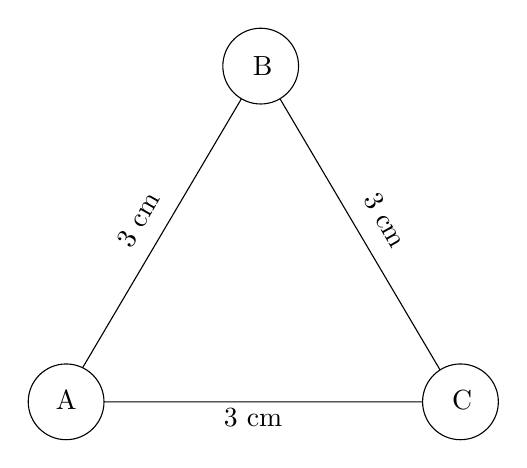
\begin{tikzpicture}[x=0.75pt,y=0.75pt,yscale=-1,xscale=1]
	\draw   (336,69) -- (431.5,230.75) -- (240.5,230.75) -- cycle ;
	\draw  [fill={rgb, 255:red, 255; green, 255; blue, 255 }  ,fill opacity=1 ] (317.75,69) .. controls (317.75,58.92) and (325.92,50.75) .. (336,50.75) .. controls (346.08,50.75) and (354.25,58.92) .. (354.25,69) .. controls (354.25,79.08) and (346.08,87.25) .. (336,87.25) .. controls (325.92,87.25) and (317.75,79.08) .. (317.75,69) -- cycle ;
	\draw  [fill={rgb, 255:red, 255; green, 255; blue, 255 }  ,fill opacity=1 ] (224,230.75) .. controls (224,220.67) and (232.17,212.5) .. (242.25,212.5) .. controls (252.33,212.5) and (260.5,220.67) .. (260.5,230.75) .. controls (260.5,240.83) and (252.33,249) .. (242.25,249) .. controls (232.17,249) and (224,240.83) .. (224,230.75) -- cycle ;
	\draw  [fill={rgb, 255:red, 255; green, 255; blue, 255 }  ,fill opacity=1 ] (414,230.75) .. controls (414,220.67) and (422.17,212.5) .. (432.25,212.5) .. controls (442.33,212.5) and (450.5,220.67) .. (450.5,230.75) .. controls (450.5,240.83) and (442.33,249) .. (432.25,249) .. controls (422.17,249) and (414,240.83) .. (414,230.75) -- cycle ;
	\draw (331,63) node [anchor=north west][inner sep=0.75pt]   [align=left] {B};
	\draw (427,224) node [anchor=north west][inner sep=0.75pt]   [align=left] {C};
	\draw (236,224) node [anchor=north west][inner sep=0.75pt]   [align=left] {A};
	\draw (264.39,153.41) node [anchor=north west][inner sep=0.75pt]  [rotate=-300] [align=left] {3 cm};
	\draw (317,233) node [anchor=north west][inner sep=0.75pt]   [align=left] {3 cm};
	\draw (393.11,127.09) node [anchor=north west][inner sep=0.75pt]  [rotate=-60] [align=left] {3 cm};
	\end{tikzpicture}
	\end{center}
\end{example}
\begin{solution}
	Observe that the triangle is equilateral, so all of its angles are $60\degr$. We want to derive a value for the net force on $B$, which consists of $F_{CB}$ and $F_{AB}$. From Coulomb's Law,
	\begin{align*}
		|F_{CB}| &= \frac{k(5\times 10^{-9}\unt{nC})(5\times 10^{-9}\unt{C})}{(0.3\unt{m})^2},
	\end{align*}
	so $|F_{CB}| = |F_{AB}| = 2.5 \times 10^{-4}\unt{N}$. Using trigonometry, we see that $F_{CBx} = -2.5\times 10^{-4}\cos(60\degr),$ or $-1.25\times 10^{-4}\unt{N}\vu{\imath}$. We also see that $F_{CBy} = -2.5\times 10^{-4}\sin(60\degr) = 2.17\times 10^{-4}\unt{N}\vu{\jmath}$. Note that $F_{ABx} = -F_{CBx}$, so adding them yields a horizontal component of 0. The vertical component is then $F_{ABy} + F_{CBy} = 2F_{CBy} = 4.34\times 10^{-4}\unt{N}\vu{\jmath}$.
	
	We know that the particle started at rest, and has an upwards force. Therefore, it will start to accelerate upwards. However, since $\frac{1}{r^2} \propto F \propto a$, acceleration will decrease as the particle gets further away.
\end{solution}

\begin{example}
	A region in space consists of three fixed point charges as in the figure below, such that $q_A = -3$ nC, $q_B = 5$ nC, and $q_C = 2$ nC. What is the net force on $q_A$? Describe it's motion.
	\begin{center}
	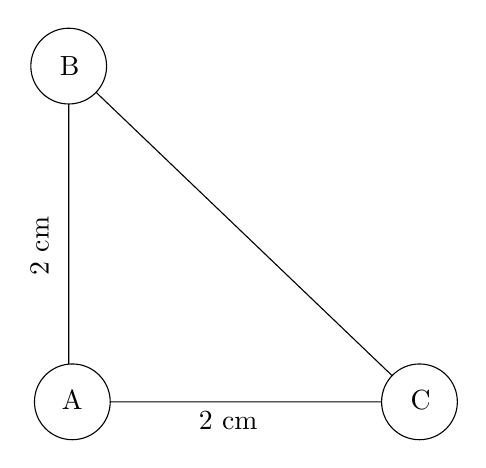
\begin{tikzpicture}[x=0.75pt,y=0.75pt,yscale=-1,xscale=1]
	\draw   (240.5,69) -- (409.5,230.75) -- (240.5,230.75) -- cycle ;
	\draw  [fill={rgb, 255:red, 255; green, 255; blue, 255 }  ,fill opacity=1 ] (222.25,69) .. controls (222.25,58.92) and (230.42,50.75) .. (240.5,50.75) .. controls (250.58,50.75) and (258.75,58.92) .. (258.75,69) .. controls (258.75,79.08) and (250.58,87.25) .. (240.5,87.25) .. controls (230.42,87.25) and (222.25,79.08) .. (222.25,69) -- cycle ;
	\draw  [fill={rgb, 255:red, 255; green, 255; blue, 255 }  ,fill opacity=1 ] (224,230.75) .. controls (224,220.67) and (232.17,212.5) .. (242.25,212.5) .. controls (252.33,212.5) and (260.5,220.67) .. (260.5,230.75) .. controls (260.5,240.83) and (252.33,249) .. (242.25,249) .. controls (232.17,249) and (224,240.83) .. (224,230.75) -- cycle ;
	\draw  [fill={rgb, 255:red, 255; green, 255; blue, 255 }  ,fill opacity=1 ] (391.25,230.75) .. controls (391.25,220.67) and (399.42,212.5) .. (409.5,212.5) .. controls (419.58,212.5) and (427.75,220.67) .. (427.75,230.75) .. controls (427.75,240.83) and (419.58,249) .. (409.5,249) .. controls (399.42,249) and (391.25,240.83) .. (391.25,230.75) -- cycle ;
	\draw (235,63) node [anchor=north west][inner sep=0.75pt]   [align=left] {B};
	\draw (404,224) node [anchor=north west][inner sep=0.75pt]   [align=left] {C};
	\draw (236,224) node [anchor=north west][inner sep=0.75pt]   [align=left] {A};
	\draw (221,171) node [anchor=north west][inner sep=0.75pt]  [rotate=-270] [align=left] {2 cm};
	\draw (302,234) node [anchor=north west][inner sep=0.75pt]   [align=left] {2 cm};
	\end{tikzpicture}
	\end{center}
\end{example}
\begin{solution}
	This is similar to the previous example. Note that the length of $BC$ is $2\sqrt{2} = 2.82$ cm, from the Pythagorean theorem. We observe that $q_B$ and $q_C$ both attract $q_A,$ such that $F_{AB} = 0.38 \times 10^{-4}\unt{N}$ and $F_{AC} = 2.25\times 10^{-4}\unt{N}$, from Coulomb's Law. Using tip-to-tail vector addition with the Pythagorean theorem, we observe that $\Sigma F = 4.0 \times 10^{-4}\unt{N}$, and $\theta = 56\degr$. This means that it will accelerate up to the right at an angle of $56\degr$, and as it does so, its acceleration will increase, and then decrease again after passing the particles.
\end{solution}

\subsection{Force of Gravity vs. Electricity}
Here, we examine gravity and electrostatics at an atomic level. Note that
\begin{equation}
	|\vb{F}_E| = \frac{kq_1q_2}{r^2}
\end{equation}
and
\begin{equation}
	|\vb{F}_G| = \frac{Gm_1m_2}{r^2}.
\end{equation}
First, we observe that both forces are vectors. However, the force of gravity can only attract, whereas $\vb{F}_E$ can attract and repel. In addition, electrostatic force concerns charge, rather than mass. Both share the property \[F \propto \frac{1}{r^2}\] up to a constant $k = 9\times 10^9$ or $G = 6.67\times 10^{-11}$. Gravity concerns larger masses and distances, whereas electrostatic force is for small charges and distances. Importantly, both of these laws define ``fields," either electric ($\vb{E}$) or gravitational ($\vb{g}$).
\begin{example}
	An electron orbits around a single proton in a hydrogen atom. Determine $\vb{F}_E$ and $\vb{F}_G$.	
\end{example}
\begin{solution}
	We know that the magnitude charge of an electron ($1.6\times10^{-19}$ C) is equal to that of a proton. The mass of an electron in $9.11\times 10^{-31}$ kg, and the mass of a proton is $1.67\times10^{-27}$ kg. Also, recall that the radius of an atom is $0.5\unt{\r{A}}$, or $0.5 \times 10^{-10}$ m. Then, we plug into the equations as follows
	\begin{equation*}
		|\vb{F}_E| = \frac{(9 \times 10^9)(1.6\times 10^{-19})(1.6\times10^{-19})}{(0.5\times 10^{-10})^2} = \boxed{9.22 \times 10^{-8}\unt{N}}
	\end{equation*}
	and
	\begin{equation*}
		|\vb{F}_G| = \frac{(6.67\times10^{-11})(1.67\times 10^{-27})(9.11\times10^{-31})}{(0.5\times 10^{-10})^2} = \boxed{4.06 \times 10^{-47}\unt{N}}.
	\end{equation*}
	Clearly, electrostatic force is much larger.
\end{solution}
\section{Electric Fields}
Electric fields are vector fields which indicate the direction and strength of the force at a particular point, as generated by one or more charged objects.
\subsection{Introduction to Electric Fields}
When we ask about electric fields, we're really asking about the nature of the attraction between two charges. In fact, we can ask a similar question with gravitation--how does the Earth's mass interact with the Sun's mass? Now, we can reorganize the equation for gravitational force such that the mass of the smaller object, $m_p$ is separate from the rest:
\begin{equation}
	|\vec{F}_g| = m_p\p{\frac{GM_e}{r^2}}.
\end{equation}
Then, let's call the quantity in parenthesis $\vec{g}$. This gives us
\begin{equation}
	\vec{F}_g = m_p\vec{g}.
\end{equation}
Notice that the field is always the same as the force. We can apply the same logic to electrostatics, so that
\begin{equation}
	\vec{F}_e = q_1\p{\frac{kq_2}{r^2}\vu{r}},
\end{equation}
where $\vu{r}$ is a radial unit vector. We then call the quantity in parenthesis $\vec{E}$, so the field is described by
\begin{equation}
	\vec{F}_e = q\vec{E}.
\end{equation}
Notice that the field and force may be in differing directions, since $q_1$ can be positive or negative. See below for some field diagrams, where the yellow dots show the strength of the field at that point.
\begin{figure}[H]
	\centering
	\includegraphics[width=0.8\textwidth]{field_notes_1}
	\caption{$\vec{E}$ generated by a positive charge}
\end{figure}
\begin{figure}[H]
	\centering
	\includegraphics[width=0.8\textwidth]{field_notes_2}
	\caption{$\vec{E}$ generated by a negative charge}
\end{figure}
We note that the electric field is equal to the force per unit charge, as in Equation~\ref{electricfieldeq}.
\begin{eqn}[Electric Field]\label{electricfieldeq}
	The electric field is given by
	\begin{equation}
		\vec{E} = \frac{\vec{F}_e}{q_s} = \frac{kq_s}{r^2}\vu{r}	
	\end{equation}
\end{eqn}
The units of electric fields are N/C. Note that the unit vector, $\vu{r}$, is a vector that points to the point from the source charge radially.
\begin{example}
	Find the electric field at $(3,4)$ from a 5 nC source charge.	
\end{example}
\begin{solution}
	Since we know $q_s$, the only thing to solve for is $r^2$. The point is at $(3,4)$ so by the distance formula, $r = \sqrt{0.03^2+0.04^2}$, or $r = 0.05$. Then, from the formula,
	\[|\vec{E}| = \frac{9\times10^9(5\times10^{-9})}{0.05^2}\vu{r},\]
	so $|\vec{E}| = 1.8\times 10^{4}\unt{N/C}$. To find the direction, we use trigonometry to find that $\theta = \tan\inv(\frac{4}{3}) = 53\degr$. Then, we use $\sint$ and $\cost$ to find that the field is given by \[\vec{E} = \boxed{1.08\times 10^4\vu{\imath} + 1.44\times 10^{4}\vu{\jmath} \unt{N/C}},\] and we're done.
\end{solution}

\subsection{Charges in Uniform Electric Fields}
In this section, we look at static equilibrium in electric fields.
\begin{example}
	What magnitude and direction of electric field is required to suspend a particle of mass 0.06 g and charge of 2 $\mu C$ in air?
\end{example}
\begin{solution}
	Since the particle must be suspended, $\Sigma F = \vec{F}_E - \vec{F}_g = 0$, where $\vec{F}_E$ points up. Thus,
	\begin{align*}
		\vec{F}_E &= \vec{F}_g \\
		q\vec{E} &= mg \\
		|\vec{E}| &= \frac{mg}{q},
	\end{align*}
	so $|\vec{E}| = 294\unt{N/C}$. For direction, we know the field is up, so $\vec{E} = 294\vu{\jmath}\unt{N/C}$.
\end{solution}
\begin{example}\label{chargeex1}
	A 2 gram ball hangs on a string in a uniform field of magnitude 1500 N/C, directed horizontally. The ball is in equilibrium when it hangs at a 30$\degr$ angle. What is its magnitude and size?
\end{example}
\begin{solution}
	We'll start with a free body diagram. Note that since $\vec{F}_T$ points to the right, $\vec{F}_E$ must point left. Thus, we have
	\begin{figure}[H]
	\centering
	\tikzset{every picture/.style={line width=0.75pt}}
	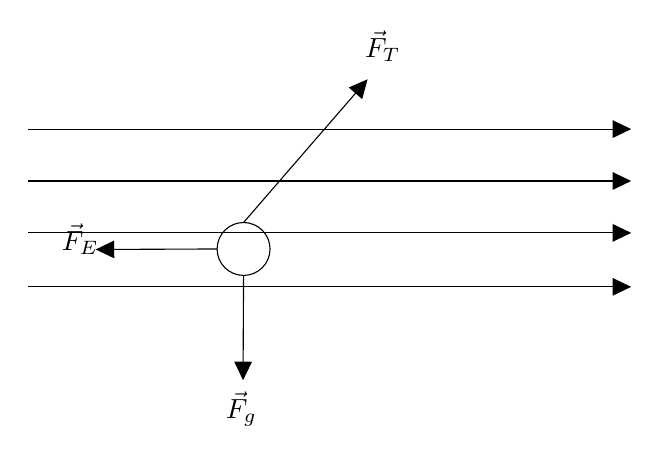
\begin{tikzpicture}[x=0.75pt,y=0.75pt,yscale=-1,xscale=1]
		\draw    (181,230) -- (468.5,230) ;
		\draw [shift={(471.5,230)}, rotate = 180] [fill={rgb, 255:red, 0; green, 0; blue, 0 }  ][line width=0.08]  [draw opacity=0] (8.93,-4.29) -- (0,0) -- (8.93,4.29) -- cycle    ;
		\draw    (181,255) -- (468.5,255) ;
		\draw [shift={(471.5,255)}, rotate = 180] [fill={rgb, 255:red, 0; green, 0; blue, 0 }  ][line width=0.08]  [draw opacity=0] (8.93,-4.29) -- (0,0) -- (8.93,4.29) -- cycle    ;
		\draw    (181,280) -- (468.5,280) ;
		\draw [shift={(471.5,280)}, rotate = 180] [fill={rgb, 255:red, 0; green, 0; blue, 0 }  ][line width=0.08]  [draw opacity=0] (8.93,-4.29) -- (0,0) -- (8.93,4.29) -- cycle    ;
		\draw    (181,306) -- (468.5,306) ;
		\draw [shift={(471.5,306)}, rotate = 180] [fill={rgb, 255:red, 0; green, 0; blue, 0 }  ][line width=0.08]  [draw opacity=0] (8.93,-4.29) -- (0,0) -- (8.93,4.29) -- cycle    ;
		\draw   (272,287.75) .. controls (272,280.71) and (277.71,275) .. (284.75,275) .. controls (291.79,275) and (297.5,280.71) .. (297.5,287.75) .. controls (297.5,294.79) and (291.79,300.5) .. (284.75,300.5) .. controls (277.71,300.5) and (272,294.79) .. (272,287.75) -- cycle ;
		\draw    (342.54,208.27) -- (284.75,275) ;
		\draw [shift={(344.5,206)}, rotate = 130.89] [fill={rgb, 255:red, 0; green, 0; blue, 0 }  ][line width=0.08]  [draw opacity=0] (8.93,-4.29) -- (0,0) -- (8.93,4.29) -- cycle    ;
		\draw    (284.75,300.5) -- (284.51,348) ;
		\draw [shift={(284.5,351)}, rotate = 270.28] [fill={rgb, 255:red, 0; green, 0; blue, 0 }  ][line width=0.08]  [draw opacity=0] (8.93,-4.29) -- (0,0) -- (8.93,4.29) -- cycle    ;
		\draw    (272,287.75) -- (216.5,287.99) ;
		\draw [shift={(213.5,288)}, rotate = 359.76] [fill={rgb, 255:red, 0; green, 0; blue, 0 }  ][line width=0.08]  [draw opacity=0] (8.93,-4.29) -- (0,0) -- (8.93,4.29) -- cycle    ;
		\draw (342,181.4) node [anchor=north west][inner sep=0.75pt]    {$\vec{F}_{T}$};
		\draw (275,355.4) node [anchor=north west][inner sep=0.75pt]    {$\vec{F}_{g}$};
		\draw (196,274.4) node [anchor=north west][inner sep=0.75pt]    {$\vec{F}_{E}$};
	\end{tikzpicture}
	\caption{Example~\ref{chargeex1}}
	\end{figure}

	\noindent Therefore, since the force on the ball is opposite to the field, the ball has negative charge. We split $\vec{F}_T$ into $\vec{F}_{Tx} = \vec{F}_T\cos(60\degr)$ and $\vec{F}_{Ty} = \vec{F}_T\sin(60\degr)$. The vertical then gives
	\begin{align*}
		\Sigma \vec{F}_y = 0 &= \vec{F}_{Ty} - \vec{F}_g \\
		F_g &= F_{T}\sin(60\degr) \\
		F_T &= \frac{F_g}{\sin(60\degr)}.
	\end{align*}
	Then, from the horizontal,
	\begin{align*}
		\Sigma \vec{F}_x = 0 &= \vec{F}_{Tx}	 - \vec{F}_E \\
		F_E &= F_T\cos(60\degr) \\
		F_E &= F_g\frac{\cos(60\degr)}{\sin(60\degr)} \\
		F_E &= mg\cot(60\degr).
	\end{align*}
	Finally, from the equation for electric field, we have
	\begin{align*}
		\vec{E} &= \frac{\vec{F}_E}{q} \\
		q &= \frac{|F_E|}{|E|} \\
		&= \frac{mg\cot(60\degr)}{|E|},
	\end{align*}
	so plugging in our values gives $q = \boxed{-7.5\times 10^{-6}\unt{C}}$.
\end{solution}
\subsection{Projectile Motion in Uniform Electric Fields}
Consider a uniform electric field, where the value of the field is equally distributed throughout an entire region. That is,
\begin{defn}[Uniform Electric Field]
	A field $\vec{E}$ is \textit{uniform} if all points $p \in \vec{E}$ have the same magnitude and direction force applied to them.	
\end{defn}
Here, we're going to examine projectile motion in such fields.
\begin{example}\label{projectilefieldex1}
	Suppose we have two plates, one positive and one negative. They create an electric field of magnitude $E$ from the positive to the negative plate. A particle is sent into the field horizontally with initial velocity $v_o$. Describe its motion.	
\end{example}
\begin{solution}
	Let's say that the particle in the field has mass $m_p$ and charge $e$ C. Launching the particle into the upward field will cause an upward force, such that the motion of the particle is parabolic, as in Figure~\ref{parabolicfieldmotion1}.
	
	\begin{figure}[H]\label{parabolicfieldmotion1}
	\centering
	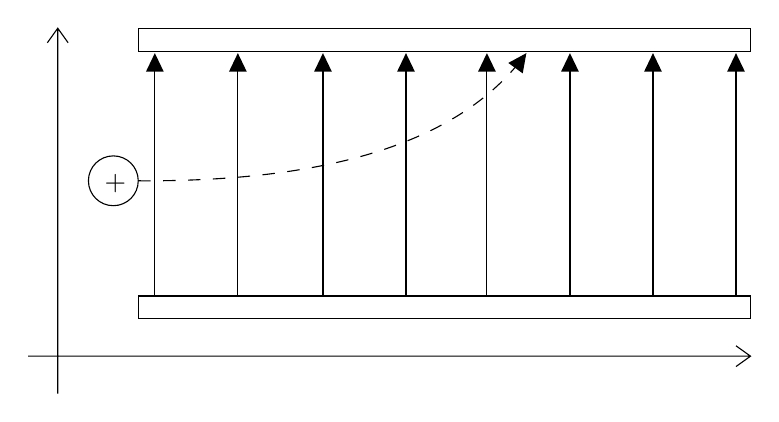
\begin{tikzpicture}[x=0.75pt,y=0.75pt,yscale=-1,xscale=1]
		\draw    (170.5,360) -- (170.5,246) ;
		\draw [shift={(170.5,243)}, rotate = 450] [fill={rgb, 255:red, 0; green, 0; blue, 0 }  ][line width=0.08]  [draw opacity=0] (8.93,-4.29) -- (0,0) -- (8.93,4.29) -- cycle    ;
		\draw    (210.5,360) -- (210.5,246) ;
		\draw [shift={(210.5,243)}, rotate = 450] [fill={rgb, 255:red, 0; green, 0; blue, 0 }  ][line width=0.08]  [draw opacity=0] (8.93,-4.29) -- (0,0) -- (8.93,4.29) -- cycle    ;
		\draw    (251.5,360) -- (251.5,246) ;
		\draw [shift={(251.5,243)}, rotate = 450] [fill={rgb, 255:red, 0; green, 0; blue, 0 }  ][line width=0.08]  [draw opacity=0] (8.93,-4.29) -- (0,0) -- (8.93,4.29) -- cycle    ;
		\draw    (291.5,360) -- (291.5,246) ;
		\draw [shift={(291.5,243)}, rotate = 450] [fill={rgb, 255:red, 0; green, 0; blue, 0 }  ][line width=0.08]  [draw opacity=0] (8.93,-4.29) -- (0,0) -- (8.93,4.29) -- cycle    ;
		\draw    (330.5,360) -- (330.5,246) ;
		\draw [shift={(330.5,243)}, rotate = 450] [fill={rgb, 255:red, 0; green, 0; blue, 0 }  ][line width=0.08]  [draw opacity=0] (8.93,-4.29) -- (0,0) -- (8.93,4.29) -- cycle    ; 
		\draw    (370.5,360) -- (370.5,246) ;
		\draw [shift={(370.5,243)}, rotate = 450] [fill={rgb, 255:red, 0; green, 0; blue, 0 }  ][line width=0.08]  [draw opacity=0] (8.93,-4.29) -- (0,0) -- (8.93,4.29) -- cycle    ;
		\draw    (410.5,360) -- (410.5,246) ;
		\draw [shift={(410.5,243)}, rotate = 450] [fill={rgb, 255:red, 0; green, 0; blue, 0 }  ][line width=0.08]  [draw opacity=0] (8.93,-4.29) -- (0,0) -- (8.93,4.29) -- cycle    ;
		\draw    (450.5,360) -- (450.5,246) ;
		\draw [shift={(450.5,243)}, rotate = 450] [fill={rgb, 255:red, 0; green, 0; blue, 0 }  ][line width=0.08]  [draw opacity=0] (8.93,-4.29) -- (0,0) -- (8.93,4.29) -- cycle    ;
		\draw   (162.5,231) -- (457.5,231) -- (457.5,242) -- (162.5,242) -- cycle ;
		\draw   (162.5,360) -- (457.5,360) -- (457.5,371) -- (162.5,371) -- cycle ;
		\draw   (138.5,304.5) .. controls (138.5,297.87) and (143.87,292.5) .. (150.5,292.5) .. controls (157.13,292.5) and (162.5,297.87) .. (162.5,304.5) .. controls (162.5,311.13) and (157.13,316.5) .. (150.5,316.5) .. controls (143.87,316.5) and (138.5,311.13) .. (138.5,304.5) -- cycle ;
		\draw  [dash pattern={on 4.5pt off 4.5pt}]  (162.5,304.5) .. controls (243.27,304.99) and (313.37,290.45) .. (347.95,245.09) ;
		\draw [shift={(349.5,243)}, rotate = 485.88] [fill={rgb, 255:red, 0; green, 0; blue, 0 }  ][line width=0.08]  [draw opacity=0] (8.93,-4.29) -- (0,0) -- (8.93,4.29) -- cycle    ;
		\draw  (109.5,389) -- (457.5,389)(123.72,231) -- (123.72,407) (450.5,384) -- (457.5,389) -- (450.5,394) (118.72,238) -- (123.72,231) -- (128.72,238)  ;
		\draw (145,300) node [anchor=north west][inner sep=0.75pt]    {$+$};
		\end{tikzpicture}	
		\caption{Example~\ref{projectilefieldex1}}
	\end{figure}
	
	\noindent Lets consider the forces acting on the particle. We know that $\Sigma F = ma$, and the only major force acting on it is $\vec{F}_E$. Thus, we have
	\begin{align*}
		\vec{F}_E &= ma \\
		q\vec{E} &= ma \\
		eE &= m_pa \\
		a &= \frac{Ee}{m_p}.	
	\end{align*}
	Now, recall our kinematics equations, which state that
	\[\Delta x = v_{xo}t + \frac{1}{2}a_xt^2.\]
	Note that in the $x$ direction, $a_x = 0$, and $x_o = 0$, giving us $x = v_ot.$ Again, let's say $y_o = 0$, and $v_{yo} = 0$. Thus,
	\[y = \frac{1}{2}\p{\frac{Ee}{m_p}}t^2.\]
	Let's now solve for $y$ as a function of $x$. We see that $t = x/v_o$, so we then have
	\[y(x) = \frac{1}{2}\p{\frac{Eex^2}{mv_o^2}},\]
	which indicates a parabolic trajectory.
\end{solution}

\section{\textbf{E} of Charge Distributions}
Here, we're interested in calculating electric fields at certain points for charge distributions, both discrete ($\Sigma$) and continuous ($\int$).

\subsection{Electric Field of a Dipole}
A dipole is a charge configuration consisting of one positive and one negative charge, as in Figure~\ref{dipolefig}, where the red charge is positive and the blue is negative.

\begin{figure}[H]\label{dipolefig}
	\centering
	\tikzset{every picture/.style={line width=0.75pt}}    
	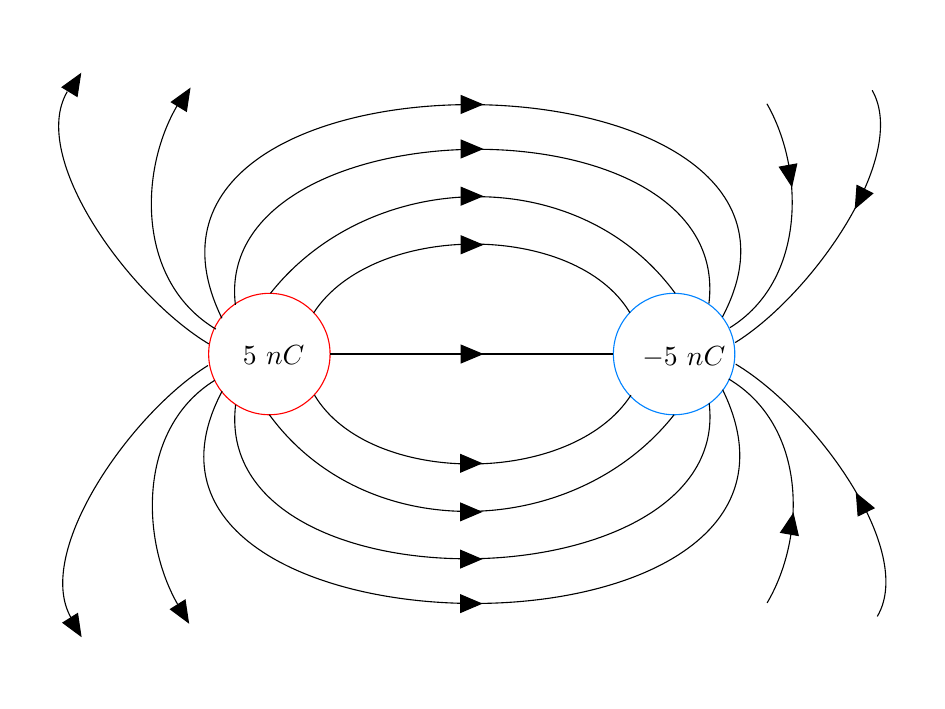
\begin{tikzpicture}[x=0.75pt,y=0.75pt,yscale=-0.65,xscale=0.65]
	\draw  [color={rgb, 255:red, 255; green, 0; blue, 0 }  ,draw opacity=1 ] (130.5,255.5) .. controls (130.5,230.65) and (150.65,210.5) .. (175.5,210.5) .. controls (200.35,210.5) and (220.5,230.65) .. (220.5,255.5) .. controls (220.5,280.35) and (200.35,300.5) .. (175.5,300.5) .. controls (150.65,300.5) and (130.5,280.35) .. (130.5,255.5) -- cycle ;
	\draw  [color={rgb, 255:red, 0; green, 130; blue, 255 }  ,draw opacity=1 ] (430.5,255.5) .. controls (430.5,230.65) and (450.65,210.5) .. (475.5,210.5) .. controls (500.35,210.5) and (520.5,230.65) .. (520.5,255.5) .. controls (520.5,280.35) and (500.35,300.5) .. (475.5,300.5) .. controls (450.65,300.5) and (430.5,280.35) .. (430.5,255.5) -- cycle ;
	\draw    (220.5,255.5) -- (430.5,255.5) ;
	\draw    (175.5,300.5) .. controls (247.5,399) and (402.5,393) .. (475.5,300.5) ;
	\draw    (209,286) .. controls (249.5,354) and (399.5,354) .. (443.5,286) ;
	\draw    (150.5,293) .. controls (131.5,449) and (519.5,442) .. (501.5,292) ;
	\draw    (140.5,283) .. controls (31.5,489) and (616.5,497) .. (511.5,282) ;
	\draw    (107.5,441) .. controls (79.5,392) and (78.5,310) .. (135,275) ;
	\draw    (28.5,451) .. controls (0.5,402) and (73.5,299) .. (130,264) ;
	\draw    (544.43,440) .. controls (573.38,391) and (574.42,309) .. (516,274) ;
	\draw    (626.11,450) .. controls (655.06,401) and (579.58,298) .. (521.17,263) ;
	\draw    (476.32,210.5) .. controls (404.32,112) and (249.32,118) .. (176.32,210.5) ;
	\draw    (442.82,225) .. controls (402.32,157) and (252.32,157) .. (208.32,225) ;
	\draw    (501.32,218) .. controls (520.32,62) and (132.32,69) .. (150.32,219) ;
	\draw    (511.32,228) .. controls (620.32,22) and (35.32,14) .. (140.32,229) ;
	\draw    (544.32,70) .. controls (572.32,119) and (573.32,201) .. (516.82,236) ;
	\draw    (622.32,60) .. controls (650.32,109) and (577.32,212) .. (520.82,247) ;
	\draw    (107.39,71) .. controls (78.44,120) and (77.4,202) .. (135.82,237) ;
	\draw    (25.71,61) .. controls (-3.24,110) and (72.24,213) .. (130.65,248) ;
	\draw  [fill={rgb, 255:red, 0; green, 0; blue, 0 }  ,fill opacity=1 ] (333.25,255.5) -- (317.75,262) -- (317.75,249) -- cycle ;
	\draw  [fill={rgb, 255:red, 0; green, 0; blue, 0 }  ,fill opacity=1 ] (333.25,174.5) -- (317.75,181) -- (317.75,168) -- cycle ;
	\draw  [fill={rgb, 255:red, 0; green, 0; blue, 0 }  ,fill opacity=1 ] (333.25,138.5) -- (317.75,145) -- (317.75,132) -- cycle ;
	\draw  [fill={rgb, 255:red, 0; green, 0; blue, 0 }  ,fill opacity=1 ] (333.25,103.5) -- (317.75,110) -- (317.75,97) -- cycle ;
	\draw  [fill={rgb, 255:red, 0; green, 0; blue, 0 }  ,fill opacity=1 ] (333.25,70.5) -- (317.75,77) -- (317.75,64) -- cycle ;
	\draw  [fill={rgb, 255:red, 0; green, 0; blue, 0 }  ,fill opacity=1 ] (332.5,336.5) -- (317.25,330) -- (317.25,343) -- cycle ;
	\draw  [fill={rgb, 255:red, 0; green, 0; blue, 0 }  ,fill opacity=1 ] (332.5,372.5) -- (317.25,366) -- (317.25,379) -- cycle ;
	\draw  [fill={rgb, 255:red, 0; green, 0; blue, 0 }  ,fill opacity=1 ] (332.5,407.5) -- (317.25,401) -- (317.25,414) -- cycle ;
	\draw  [fill={rgb, 255:red, 0; green, 0; blue, 0 }  ,fill opacity=1 ] (332.5,440.5) -- (317.25,434) -- (317.25,447) -- cycle ;
	
	\draw  [fill={rgb, 255:red, 0; green, 0; blue, 0 }  ,fill opacity=1 ] (116.54,58.89) -- (114,75.5) -- (102.91,68.72) -- cycle ;
	\draw  [fill={rgb, 255:red, 0; green, 0; blue, 0 }  ,fill opacity=1 ] (35.54,47.89) -- (33,64.5) -- (21.91,57.72) -- cycle ;
	\draw  [fill={rgb, 255:red, 0; green, 0; blue, 0 }  ,fill opacity=1 ] (115.5,454.5) -- (113.03,437.89) -- (102.25,444.67) -- cycle ;
	\draw  [fill={rgb, 255:red, 0; green, 0; blue, 0 }  ,fill opacity=1 ] (35.8,464.5) -- (33.32,447.89) -- (22.54,454.67) -- cycle ;
	\draw  [fill={rgb, 255:red, 0; green, 0; blue, 0 }  ,fill opacity=1 ] (562.75,131.02) -- (553.59,116.92) -- (566.39,114.61) -- cycle ;
	\draw  [fill={rgb, 255:red, 0; green, 0; blue, 0 }  ,fill opacity=1 ] (609.85,147.3) -- (611.09,130.54) -- (622.68,136.43) -- cycle ;
	\draw  [fill={rgb, 255:red, 0; green, 0; blue, 0 }  ,fill opacity=1 ] (563.8,373.94) -- (554.5,387.74) -- (567.5,390) -- cycle ;
	\draw  [fill={rgb, 255:red, 0; green, 0; blue, 0 }  ,fill opacity=1 ] (610.65,359) -- (611.91,375.41) -- (623.68,369.64) -- cycle ;
	\draw (154,247.4) node [anchor=north west][inner sep=0.75pt]    {$5\ nC$};
	\draw (450,248.4) node [anchor=north west][inner sep=0.75pt]    {$-5\ nC$};
	\end{tikzpicture}
	\caption{An Electric Dipole}
\end{figure}

Note that here, the field lines are no longer radially extended. Instead, they point out from the positive charge and curve to meet the negative charge. Also notice that this diagram uses connected lines, rather than a vector field, to indicate the direction.
\begin{question}
	What the the electric field at a specific point around the dipole?	
\end{question}
To answer this, let's start with a numerical example.
\begin{example}\label{dipoleexample}
	What is the net electric field at the point $(3,0)$ from the charge configuration shown below?
\end{example}
\begin{figure}[H]
	\centering
	\begin{tikzpicture}[x=0.75pt,y=0.75pt,yscale=-1,xscale=1]
	\draw  (74.5,141) -- (511.5,141)(131.5,20) -- (131.5,280) (504.5,136) -- (511.5,141) -- (504.5,146) (126.5,27) -- (131.5,20) -- (136.5,27)  ;
	\draw  [fill={rgb, 255:red, 255; green, 255; blue, 255 }  ,fill opacity=1 ] (339.5,141.25) .. controls (339.5,137.25) and (342.75,134) .. (346.75,134) .. controls (350.75,134) and (354,137.25) .. (354,141.25) .. controls (354,145.25) and (350.75,148.5) .. (346.75,148.5) .. controls (342.75,148.5) and (339.5,145.25) .. (339.5,141.25) -- cycle ;
	\draw  [color={rgb, 255:red, 255; green, 0; blue, 0 }  ,draw opacity=1 ][fill={rgb, 255:red, 255; green, 255; blue, 255 }  ,fill opacity=1 ] (106,82.25) .. controls (106,67.48) and (117.98,55.5) .. (132.75,55.5) .. controls (147.52,55.5) and (159.5,67.48) .. (159.5,82.25) .. controls (159.5,97.02) and (147.52,109) .. (132.75,109) .. controls (117.98,109) and (106,97.02) .. (106,82.25) -- cycle ;
	\draw  [color={rgb, 255:red, 71; green, 146; blue, 255 }  ,draw opacity=1 ][fill={rgb, 255:red, 255; green, 255; blue, 255 }  ,fill opacity=1 ] (105,210.25) .. controls (105,195.48) and (116.98,183.5) .. (131.75,183.5) .. controls (146.52,183.5) and (158.5,195.48) .. (158.5,210.25) .. controls (158.5,225.02) and (146.52,237) .. (131.75,237) .. controls (116.98,237) and (105,225.02) .. (105,210.25) -- cycle ;
	\draw (117,76) node [anchor=north west][inner sep=0.75pt]    {$5\ nC$};
	\draw (111,205) node [anchor=north west][inner sep=0.75pt]    {$-5\ nC$};
	\draw (323,151.4) node [anchor=north west][inner sep=0.75pt]    {$x=3\mathrm{m}$};
	\draw (47,76) node [anchor=north west][inner sep=0.75pt]    {$y=1\mathrm{m}$};
	\draw (48,205) node [anchor=north west][inner sep=0.75pt]    {$y=1\mathrm{m}$};
	\end{tikzpicture}
	\caption{Example~\ref{dipoleexample}}
\end{figure}

\begin{solution}
	We start by finding the magnitude of the field between the point and $q_1$. Note that we can use the Pythagorean Theorem to find $r$, such that
	\[r^2 = 1^2 + 3^2 = 10.\]
	Then, from the equation for electric field,
	\begin{align*}
		\vec{E}_1 &= \frac{kq}{r^2}\vu{r} \\
		&= \frac{(9\times 10^9)(5\times 10^{-9})}{10}\vu{r}.
	\end{align*}
	Using vector addition, note that again from the Pythagorean Theorem,
	\[\vu{r} = \frac{3\sqrt{10}}{10}\vu{\imath} - \frac{\sqrt{10}}{10}\vu{\jmath}.\]
	Thus, by substituting and distributing we have
	\[\vec{E}_1 = 4.27\vu{\imath} - 1.42\vu{\jmath} \unt{N/C}.\]
	Now, we consider the second charge. Again, this is similar, but $q_2$ is negative, and
	\[\vu{r} = \frac{3\sqrt{10}}{10}\vu{\imath} + \frac{\sqrt{10}}{10}\vu{\jmath}.\]
	Then, we have
	\[\vec{E}_2 = -4.27\vu{\imath} - 1.42\vu{\jmath}\unt{N/C}.\]
	Note that intuitively, the $\vu{\imath}$ components cancel out. Adding $\vec{E}_1$ and $\vec{E}_2$ gives
	\[\Sigma \vec{E} = 0\vu{\imath} - 2.84\vu{\jmath}\unt{N/C},\]
	and we're done.
\end{solution}
Now that we have this in mind, let's solve this in a general case, where we want to find the field at a point $(x, 0)$, where the two charges have magnitude $q$ and $-q$ respectively, and are placed at $y$ and $-y$. This is relatively simple. Now, we find that $r$ is given by
	\[\vu{r} = \sqrt{x^2 + y^2}.\]
	To evaluate $\vu{r}$, we use the same approach as in the example, so
	\[\vu{r}_1 = \frac{x}{\sqrt{x^2+y^2}}\vu{\imath} - \frac{y}{\sqrt{x^2+y^2}}\vu{\jmath}.\]
	For $q_2$, we have the same, except the $\vu{\jmath}$ component is positive. This gives
	\begin{align*}
		\vec{E}_1 &= \frac{kqx}{\sqrt{(x^2+y^2)^3}}\vu{\imath} + \frac{kqy}{\sqrt{(x^2+y^2)^3}}\vu{\jmath} \\
		\vec{E}_2 &= -\frac{kqx}{\sqrt{(x^2+y^2)^3}}\vu{\imath} - \frac{kqy}{\sqrt{(x^2+y^2)^3}}\vu{\jmath}.
	\end{align*}
	Adding, again, yields
	\[\Sigma \vec{E} = -\frac{2kqy}{\sqrt{(x^2+y^2)^3}}\vu{\jmath}.\]
	Consider the limit as $y$ goes to $0$. That is, what happens when the charges both lie at the origin? Taking the limit gives
	\begin{align*}
		\lim_{y\to 0} \vec{E} &= -\lim_{y\to 0}\frac{2kqy}{\sqrt{(x^2+y^2)^3}}\vu{\jmath} \\
		&= -\frac{\lim_{y\to 0} 2kqy}{\lim_{y\to 0}\sqrt{(x^2+y^2)^3}} \\
		&= \frac{0}{x^3},
	\end{align*}
	which evaluates to 0. Now, consider the limit as $x$ goes to 0. Here, the denominator becomes $y^3$ and cancels with the numerator, so that
	\[\lim_{x\to 0} \vec{E} = -\frac{2kq}{y^2}.\]
\subsection{Electric Field of a Rod}
Here, we'll use integration to derive the electric field for a charged rod.
\begin{example}\label{chargedrodfieldex}
	A positively charged rod of length $L$ lies a distance $A$ from the origin, as in the figure below. Find the electric field ata  point a distance $A$ from the left end. Then, evaluate the electric field value when $A \gg L$.	
\end{example}

\begin{figure}[H]
	\centering
	\begin{tikzpicture}[x=0.75pt,y=0.75pt,yscale=-1,xscale=1]
	\draw  (73.5,89.52) -- (510.5,89.52)(128.5,20) -- (128.5,165) (503.5,84.52) -- (510.5,89.52) -- (503.5,94.52) (123.5,27) -- (128.5,20) -- (133.5,27)  ;
	\draw  [fill={rgb, 255:red, 255; green, 255; blue, 255 }  ,fill opacity=1 ] (173.25,82) -- (402.25,82) .. controls (403.49,82) and (404.5,85.36) .. (404.5,89.5) .. controls (404.5,93.64) and (403.49,97) .. (402.25,97) -- (173.25,97) .. controls (172.01,97) and (171,93.64) .. (171,89.5) .. controls (171,85.36) and (172.01,82) .. (173.25,82) .. controls (174.49,82) and (175.5,85.36) .. (175.5,89.5) .. controls (175.5,93.64) and (174.49,97) .. (173.25,97) ;
	\draw    (171,89.5) -- (175.5,89.5) ;
	\draw (141,92.4) node [anchor=north west][inner sep=0.75pt]    {$A$};
	\draw (267,58.4) node [anchor=north west][inner sep=0.75pt]    {$L$};
	\end{tikzpicture}
	\caption{Example~\ref{chargedrodfieldex}}
\end{figure}

\begin{solution}
	Consider the same setup, but instead, with a point at a distance $A$ from the origin. Here, we just use the electric field equation $\vec{E} = q\vec{F}_E$. Expressing the distance as $x$, we have
	\begin{align*}
		\vec{E} &= \frac{kq}{r^2}\vu{r} \\
		&= -\frac{kq}{x^2}\vu{\imath}.
	\end{align*}
	Now suppose we continually add points some slight distance from $A$, until we form a length of $L$. Here, suppose that the rod has some small sub-charge $\dd q$, which generates a field $\dd E$. Again, we have
	\begin{align*}
		\vec{E} &= \frac{kq}{r^2}\vu{r} \\
		\dd\vec{E} &= -\frac{k\dd q}{r^2}\vu{\imath}.	
	\end{align*}
	Note that here, $r = $. Integrating yields
	\begin{equation*}
		\int \dd \vec{E} = -\int_{A}^{A+L} \frac{k\dd q}{r^2}\vu{\imath}.
	\end{equation*}
	Of course, we can't integrate position with respect to charge. Using uniform linear density $\lambda$ gives us
	\[\lambda \equiv \frac{Q}{L} = \dv{q}{x}.\]
	Multiplying by $\dd x$ gives us $\dd q = \lambda\dd x$, so we have
	\begin{align*}
		\vec{E} &= -\int_A^{A+L} \frac{k\lambda\dd x}{x^2}\vu{\imath} \\
		&= -k\lambda \int_A^{A+L} \frac{1}{x^2}\dd x \vu{\imath} \\
		&= -k\lambda\p{-\frac{1}{x}\big|_{A}^{L+A}}\vu{\imath} \\
		&= k\lambda\p{\frac{1}{L+A} - \frac{1}{A}} \\
		&= \boxed{-\frac{kQ}{A(L+A)}}.
	\end{align*}
	Now, let's suppose that $A \gg L$. In this case, $L$ is negligible, giving us
	\[\vec{E} = -\frac{kQ}{A^2},\]
	and we're done.
\end{solution}
\section{Gauss's Law and Electric Flux}
Gauss's law, named after Carl Friedrich Gauss (who formulated it in 1813), is one of Maxwell's four equations for electromagnetism. It comes as a direct result of Coulomb's Law, but provides an easier framework for calculating the electric field of charge distributions.
\subsection{Introduction to Flux}
Recall that an electric field line is a line in space such that any point tangent to it points in the direction of the field at that location, such as in Figure~\ref{elecfieldtangentfig}.

\begin{figure}[H]
	\centering
	\tikzset{every picture/.style={line width=0.75pt}}
	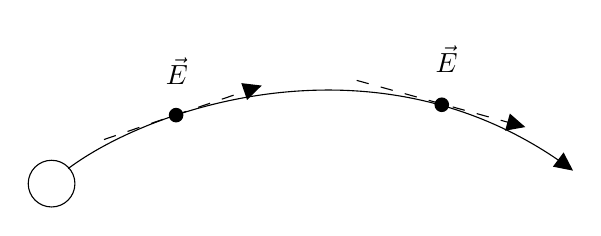
\begin{tikzpicture}[x=0.75pt,y=0.75pt,yscale=-1,xscale=1]
	\draw   (78,146.25) .. controls (78,140.04) and (83.04,135) .. (89.25,135) .. controls (95.46,135) and (100.5,140.04) .. (100.5,146.25) .. controls (100.5,152.46) and (95.46,157.5) .. (89.25,157.5) .. controls (83.04,157.5) and (78,152.46) .. (78,146.25) -- cycle ;
	\draw  [fill={rgb, 255:red, 0; green, 0; blue, 0 }  ,fill opacity=1 ] (146,113.25) .. controls (146,111.46) and (147.46,110) .. (149.25,110) .. controls (151.04,110) and (152.5,111.46) .. (152.5,113.25) .. controls (152.5,115.04) and (151.04,116.5) .. (149.25,116.5) .. controls (147.46,116.5) and (146,115.04) .. (146,113.25) -- cycle ;
	\draw  [fill={rgb, 255:red, 0; green, 0; blue, 0 }  ,fill opacity=1 ] (274,108.25) .. controls (274,106.46) and (275.46,105) .. (277.25,105) .. controls (279.04,105) and (280.5,106.46) .. (280.5,108.25) .. controls (280.5,110.04) and (279.04,111.5) .. (277.25,111.5) .. controls (275.46,111.5) and (274,110.04) .. (274,108.25) -- cycle ;
	\draw    (97.25,139) .. controls (137.05,109.15) and (247.39,71.38) .. (339.12,138.97) ;
	\draw [shift={(340.5,140)}, rotate = 216.87] [fill={rgb, 255:red, 0; green, 0; blue, 0 }  ][line width=0.08]  [draw opacity=0] (8.93,-4.29) -- (0,0) -- (8.93,4.29) -- cycle    ;
	\draw  [dash pattern={on 4.5pt off 4.5pt}]  (114.5,125) -- (187.66,99.97) ;
	\draw [shift={(190.5,99)}, rotate = 521.11] [fill={rgb, 255:red, 0; green, 0; blue, 0 }  ][line width=0.08]  [draw opacity=0] (8.93,-4.29) -- (0,0) -- (8.93,4.29) -- cycle    ;
	\draw  [dash pattern={on 4.5pt off 4.5pt}]  (236.25,96.5) -- (314.61,118.2) ;
	\draw [shift={(317.5,119)}, rotate = 195.48] [fill={rgb, 255:red, 0; green, 0; blue, 0 }  ][line width=0.08]  [draw opacity=0] (8.93,-4.29) -- (0,0) -- (8.93,4.29) -- cycle    ;
	\draw (143,84.4) node [anchor=north west][inner sep=0.75pt]    {$\vec{E}$};
	\draw (273,78.4) node [anchor=north west][inner sep=0.75pt]    {$\vec{E}$};
	\end{tikzpicture}
	\caption{Electric Field Lines}\label{elecfieldtangentfig}
\end{figure}

\noindent Using this, we define \textit{flux} as
\begin{defn}[Electric Flux]
	The electric flux, $\Phi$, is the amount of field lines flowing through an area, such that
	\begin{equation}\label{fluxeqdotted}
		\Phi = \vec{E}\cdot\vec{A},
	\end{equation}
	where $\vec{A}$ is the area vector.
\end{defn}
Note that here, area is a vector such that $\vec{A} = A\vec{n}$ where $\vec{n}$ is a normal vector. This then indicates that flux is a scalar quantity. We can also write flux as
\begin{equation}\label{fluxeqcos}
	\Phi = |E||A|\cos\theta,
\end{equation}
from the definition of a dot product.
\begin{example}\label{diskfluxex1}
	A disk of radius 0.25 m is in a region of a uniform electric field with 	magnitude 3000 N/C. What is the flux through the disk, given that its unit vector makes a 30 degree angle with the field? What angle should the disk be rotated to in order to maximize flux, and what is $\max\Phi$?
\end{example}
\begin{figure}[H]
	\centering
	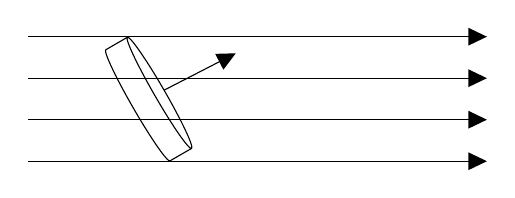
\begin{tikzpicture}[x=0.75pt,y=0.75pt,yscale=-1,xscale=1]
	\draw    (100.5,110) -- (318.5,110) ;
	\draw [shift={(321.5,110)}, rotate = 180] [fill={rgb, 255:red, 0; green, 0; blue, 0 }  ][line width=0.08]  [draw opacity=0] (8.93,-4.29) -- (0,0) -- (8.93,4.29) -- cycle    ;
	\draw    (100.5,130) -- (318.5,130) ;
	\draw [shift={(321.5,130)}, rotate = 180] [fill={rgb, 255:red, 0; green, 0; blue, 0 }  ][line width=0.08]  [draw opacity=0] (8.93,-4.29) -- (0,0) -- (8.93,4.29) -- cycle    ;
	\draw    (100.5,150) -- (318.5,150) ;
	\draw [shift={(321.5,150)}, rotate = 180] [fill={rgb, 255:red, 0; green, 0; blue, 0 }  ][line width=0.08]  [draw opacity=0] (8.93,-4.29) -- (0,0) -- (8.93,4.29) -- cycle    ;
	\draw    (100.5,170) -- (318.5,170) ;
	\draw [shift={(321.5,170)}, rotate = 180] [fill={rgb, 255:red, 0; green, 0; blue, 0 }  ][line width=0.08]  [draw opacity=0] (8.93,-4.29) -- (0,0) -- (8.93,4.29) -- cycle    ;
	\draw   (179.19,163.83) -- (168.8,169.83) .. controls (167.57,170.54) and (159.66,159.12) .. (151.12,144.34) .. controls (142.58,129.55) and (136.66,116.99) .. (137.89,116.28) -- (148.27,110.29) .. controls (149.5,109.58) and (157.42,120.99) .. (165.96,135.77) .. controls (174.49,150.56) and (180.42,163.12) .. (179.19,163.83) .. controls (177.96,164.54) and (170.04,153.13) .. (161.51,138.34) .. controls (152.97,123.56) and (147.04,110.99) .. (148.27,110.29) ;
	\draw    (165.96,135.77) -- (197.83,119.37) ;
	\draw [shift={(200.5,118)}, rotate = 512.77] [fill={rgb, 255:red, 0; green, 0; blue, 0 }  ][line width=0.08]  [draw opacity=0] (8.93,-4.29) -- (0,0) -- (8.93,4.29) -- cycle    ;
	\end{tikzpicture}
	\caption{Example~\ref{diskfluxex1}}
\end{figure}
\begin{solution}
	Observe that the area of the disk is simply $\pi r^2$, where $r= 0.25$. Then, we can use Equation~\ref{fluxeqcos} to say
	\[\Phi = 3000\pi(0.25)^2\cos(30\degr),\]
	so $\Phi = \boxed{510 \unt{Nm$^2$/C}}$ (note the units). To maximize flux, we want to maximize $\cos\theta$, meaning that $\theta = 0\degr$. Thus, we have
	\[\max\Phi = 3000\pi(0.25)^2\cos 0,\]
	or $\boxed{589\unt{Nm$^2$/C}}$. To minimize flux, we have $\min\cost = 0$, so $\min\Phi = 0$.
\end{solution}
Here, we've only focused on the electric field flowing through a flat surface. However, we should also consider \textit{closed surfaces}. Consider a sphere with a positive point charge in the middle, such that the charge creates an electric field outwards from the sphere. If the electric field through some small $\dd \vec{A}$ is not the same as the field through another $\dd \vec{A}$, we need to write a modified expression for flux.
\begin{eqn}[Integral Form of Gauss's Law]
	The flux of a closed surface is
	\begin{equation}
		\Phi = \oint \vec{E}\cdot\dd \vec{A}.
	\end{equation}
\end{eqn}
The $\oint$ integral is a \textit{surface integral}, which means that the integral must be over a closed surface. Recall that
\[|E| = \frac{q}{4\pi\eps_0r^2},\]
where $\eps_0$ is the permittivity of free space. Observe that since $r$ is constant in the above scenario, $|\vec{E}|$ is also constant, and can be pulled out of our integral (along with the dot product), such that
\begin{align*}
	\Phi &= \vec{E}\cos(0)\oint \dd \vec{A} \\
	&= \frac{1}{4\pi\eps_0}\oint \dd \vec{A}.	
\end{align*}
Since the surface area of a sphere is $4\pi r^2$, we have\[\oint \dd \vec{A} = 4\pi r^2,\] so the above expression transforms into
\begin{eqn}[Gauss's Law]
	For a closed surface with charge $q$,
	\[\Phi = \frac{q}{\eps_0}.\]
\end{eqn}
Suppose we now bring in an external charge to this sphere. The field lines of this external charge will enter the surface and leave the surface, meaning that they will bring an external flux of 0. Therefore, the net flux is still equal to in enclosed charge divided by $\eps_0$.
\begin{example}\label{gaussiansurfaceex}
	Rank the Gaussian surfaces in Figure~\ref{gaussiansurfaceexfig} from most positive $\Phi_{\text{net}}$ to most negative $\Phi_{\text{net}}$.	
\end{example}
\begin{solution}
	These surfaces are called \textit{Gaussian} as they are closed 3D surfaces. To calculate the flux, we need to know the charge enclosed by each surface. For surface $A$, note that only a $+2$ charge is enclosed, and in $B$, only a $-7$ charge is enclosed. In $C$, we have $+2$, $-3$, and $-7$ enclosed, giving us a $-8$ charge. Thus we have $\Phi_A > \Phi_B > \Phi_C$.
\end{solution}
\begin{figure}[H]
	\centering
	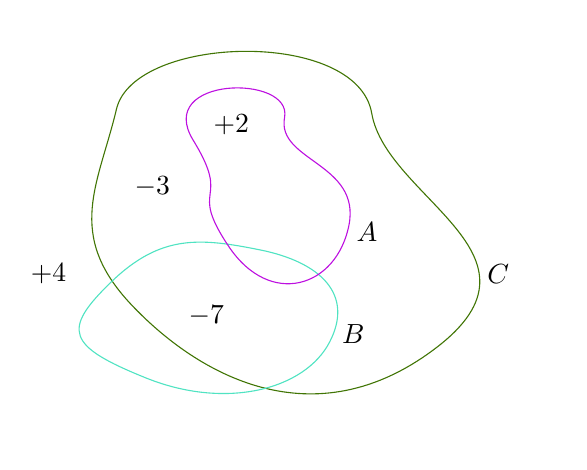
\begin{tikzpicture}[x=0.75pt,y=0.75pt,yscale=-1,xscale=1]
	\draw  [color={rgb, 255:red, 65; green, 117; blue, 5 }  ,draw opacity=1 ] (218.5,89) .. controls (227,53) and (334.5,50) .. (341.5,91) .. controls (348.5,132) and (431.5,159) .. (372.5,204) .. controls (313.5,249) and (257.5,217) .. (225.5,183) .. controls (193.5,149) and (210,125) .. (218.5,89) -- cycle ;
	\draw  [color={rgb, 255:red, 80; green, 227; blue, 194 }  ,draw opacity=1 ] (216,172.23) .. controls (239.92,149.1) and (259.05,151.03) .. (287.75,156.81) .. controls (316.45,162.59) and (333.19,178.02) .. (321.23,201.15) .. controls (309.27,224.29) and (271.01,233.93) .. (232.74,218.5) .. controls (194.48,203.08) and (192.09,195.37) .. (216,172.23) -- cycle ;
	\draw  [color={rgb, 255:red, 189; green, 16; blue, 224 }  ,draw opacity=1 ] (255.5,104) .. controls (236.5,73) and (303.5,72) .. (299.5,93) .. controls (295.5,114) and (336.5,115) .. (330.5,145) .. controls (324.5,175) and (292.5,185) .. (272.5,155) .. controls (252.5,125) and (274.5,135) .. (255.5,104) -- cycle ;
	\draw (333,142.4) node [anchor=north west][inner sep=0.75pt]    {$A$};
	\draw (326,191.4) node [anchor=north west][inner sep=0.75pt]    {$B$};
	\draw (396,162.4) node [anchor=north west][inner sep=0.75pt]    {$C$};
	\draw (264,90.4) node [anchor=north west][inner sep=0.75pt]    {$+2$};
	\draw (252,182.4) node [anchor=north west][inner sep=0.75pt]    {$-7$};
	\draw (176,162.4) node [anchor=north west][inner sep=0.75pt]    {$+4$};
	\draw (226,120.4) node [anchor=north west][inner sep=0.75pt]    {$-3$};
	\end{tikzpicture}
	\caption{Example~\ref{gaussiansurfaceex}}\label{gaussiansurfaceexfig}
\end{figure}
\subsection{Electric Field of a Rod}
Here, we're going to find the electric field of a uniformly charged rod using Gauss's Law. Consider the rod in Figure~\ref{uniformrodgaussfig1}.
\begin{figure}[H]
	\centering
	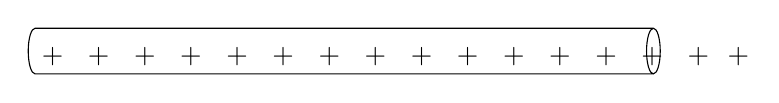
\begin{tikzpicture}[x=0.75pt,y=0.75pt,yscale=-1,xscale=1]
	\draw   (471.2,153) -- (173.3,153) .. controls (171.48,153) and (170,148.08) .. (170,142) .. controls (170,135.92) and (171.48,131) .. (173.3,131) -- (471.2,131) .. controls (473.02,131) and (474.5,135.92) .. (474.5,142) .. controls (474.5,148.08) and (473.02,153) .. (471.2,153) .. controls (469.38,153) and (467.9,148.08) .. (467.9,142) .. controls (467.9,135.92) and (469.38,131) .. (471.2,131) ;
	\draw (175.3,139) node [anchor=north west][inner sep=0.75pt]    {$+\ \ +\ \ +\ \ +\ \ +\ \ +\ \ +\ \ +\ \ +\ \ +\ \ +\ \ +\ \ +\ \ +\ \ +\ \ +$};
	\end{tikzpicture}
	\caption{Uniform Rod}\label{uniformrodgaussfig1}
\end{figure}

Examine the electric field generated by this rod. The electric field will point radially outwards from the rod, since it has positive charge. Say that the rod has length $L$ and total charge $Q$. The rod is effectively a closed cylinder from a Gaussian perspective, since the electric field lines mimic an enclosed surface. Note that $\dd \vec{A} \parallel \vec{E}$, so that $\theta = 0$ and $\cost = 1$ in the middle of the cylinder. At the ends of the cylinder, however, $\dd\vec{A} \perp \vec{E}$, so $\cost = 0$. Then, we have
\[\Phi_{\text{end}} + \Phi_{\text{end}} + \Phi_{\text{mid}} = \frac{q_{en}}{\eps_0}.\]
Since $\Phi_{\text{end}} = 0$, we have $\Phi_{\text{mid}} = Q/\eps_0$. From Gauss's law,
\begin{align*}
	\oint \vec{E} \dd \vec{A} &= \frac{q_{en}}{\eps_0} \\
	\vec{E}\cdot A &= \frac{q_{en}}{\eps_0} \\
	\vec{E}(2\pi x\ell) &= \frac{q_{en}}{\eps_0}.
\end{align*}
Since the rod is uniformly charged,
\[\lambda = \frac{Q}{L} = \frac{q_{en}}{\ell},\]
where $\ell$ is the length of the Gaussian cylinder. Using $q_{en} = \lambda\ell$ gives us
\begin{align*}
	2\pi x \ell\vec{E} &= \frac{\lambda\ell}{\eps_0} \\
	\vec{E} &= \frac{\lambda}{2\pi \eps_0 x} \\
	&= \frac{Q}{2L\pi\eps_0x}
\end{align*}
Note that $\lim\limits_{x\to \infty}\vec{E} = 0$.
\subsection{Electric Field of a Plane}
Consider a plane as in Figure~\ref{uniformplategaussfig1}.
\begin{figure}[H]
	\centering
	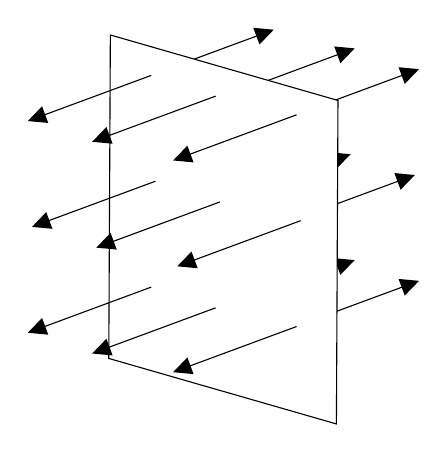
\begin{tikzpicture}[x=0.75pt,y=0.75pt,yscale=-1,xscale=1]
	\draw    (339.5,191) -- (396.19,170.04) ;
	\draw [shift={(399,169)}, rotate = 519.71] [fill={rgb, 255:red, 0; green, 0; blue, 0 }  ][line width=0.08]  [draw opacity=0] (8.93,-4.29) -- (0,0) -- (8.93,4.29) -- cycle    ;
	\draw    (308.5,181) -- (365.19,160.04) ;
	\draw [shift={(368,159)}, rotate = 519.71] [fill={rgb, 255:red, 0; green, 0; blue, 0 }  ][line width=0.08]  [draw opacity=0] (8.93,-4.29) -- (0,0) -- (8.93,4.29) -- cycle    ;
	\draw    (269.5,172) -- (326.19,151.04) ;
	\draw [shift={(329,150)}, rotate = 519.71] [fill={rgb, 255:red, 0; green, 0; blue, 0 }  ][line width=0.08]  [draw opacity=0] (8.93,-4.29) -- (0,0) -- (8.93,4.29) -- cycle    ;
	\draw    (337.5,140) -- (394.19,119.04) ;
	\draw [shift={(397,118)}, rotate = 519.71] [fill={rgb, 255:red, 0; green, 0; blue, 0 }  ][line width=0.08]  [draw opacity=0] (8.93,-4.29) -- (0,0) -- (8.93,4.29) -- cycle    ;
	\draw    (306.5,130) -- (363.19,109.04) ;
	\draw [shift={(366,108)}, rotate = 519.71] [fill={rgb, 255:red, 0; green, 0; blue, 0 }  ][line width=0.08]  [draw opacity=0] (8.93,-4.29) -- (0,0) -- (8.93,4.29) -- cycle    ;
	\draw    (267.5,121) -- (324.19,100.04) ;
	\draw [shift={(327,99)}, rotate = 519.71] [fill={rgb, 255:red, 0; green, 0; blue, 0 }  ][line width=0.08]  [draw opacity=0] (8.93,-4.29) -- (0,0) -- (8.93,4.29) -- cycle    ;
	\draw    (339.5,89) -- (396.19,68.04) ;
	\draw [shift={(399,67)}, rotate = 519.71] [fill={rgb, 255:red, 0; green, 0; blue, 0 }  ][line width=0.08]  [draw opacity=0] (8.93,-4.29) -- (0,0) -- (8.93,4.29) -- cycle    ;
	\draw    (308.5,79) -- (365.19,58.04) ;
	\draw [shift={(368,57)}, rotate = 519.71] [fill={rgb, 255:red, 0; green, 0; blue, 0 }  ][line width=0.08]  [draw opacity=0] (8.93,-4.29) -- (0,0) -- (8.93,4.29) -- cycle    ;
	\draw    (269.5,70) -- (326.19,49.04) ;
	\draw [shift={(329,48)}, rotate = 519.71] [fill={rgb, 255:red, 0; green, 0; blue, 0 }  ][line width=0.08]  [draw opacity=0] (8.93,-4.29) -- (0,0) -- (8.93,4.29) -- cycle    ;
	\draw  [fill={rgb, 255:red, 255; green, 255; blue, 255 }  ,fill opacity=1 ] (359.19,237.94) -- (359.95,82.09) -- (250.28,50.54) -- (249.52,206.38) -- cycle ;
	\draw    (270,70) -- (213.31,90.96) ;
	\draw [shift={(210.5,92)}, rotate = 339.71000000000004] [fill={rgb, 255:red, 0; green, 0; blue, 0 }  ][line width=0.08]  [draw opacity=0] (8.93,-4.29) -- (0,0) -- (8.93,4.29) -- cycle    ;
	\draw    (301,80) -- (244.31,100.96) ;
	\draw [shift={(241.5,102)}, rotate = 339.71000000000004] [fill={rgb, 255:red, 0; green, 0; blue, 0 }  ][line width=0.08]  [draw opacity=0] (8.93,-4.29) -- (0,0) -- (8.93,4.29) -- cycle    ;
	\draw    (340,89) -- (283.31,109.96) ;
	\draw [shift={(280.5,111)}, rotate = 339.71000000000004] [fill={rgb, 255:red, 0; green, 0; blue, 0 }  ][line width=0.08]  [draw opacity=0] (8.93,-4.29) -- (0,0) -- (8.93,4.29) -- cycle    ;
	\draw    (272,121) -- (215.31,141.96) ;
	\draw [shift={(212.5,143)}, rotate = 339.71000000000004] [fill={rgb, 255:red, 0; green, 0; blue, 0 }  ][line width=0.08]  [draw opacity=0] (8.93,-4.29) -- (0,0) -- (8.93,4.29) -- cycle    ;
	\draw    (303,131) -- (246.31,151.96) ;
	\draw [shift={(243.5,153)}, rotate = 339.71000000000004] [fill={rgb, 255:red, 0; green, 0; blue, 0 }  ][line width=0.08]  [draw opacity=0] (8.93,-4.29) -- (0,0) -- (8.93,4.29) -- cycle    ;
	\draw    (342,140) -- (285.31,160.96) ;
	\draw [shift={(282.5,162)}, rotate = 339.71000000000004] [fill={rgb, 255:red, 0; green, 0; blue, 0 }  ][line width=0.08]  [draw opacity=0] (8.93,-4.29) -- (0,0) -- (8.93,4.29) -- cycle    ;
	\draw    (270,172) -- (213.31,192.96) ;
	\draw [shift={(210.5,194)}, rotate = 339.71000000000004] [fill={rgb, 255:red, 0; green, 0; blue, 0 }  ][line width=0.08]  [draw opacity=0] (8.93,-4.29) -- (0,0) -- (8.93,4.29) -- cycle    ;
	\draw    (301,182) -- (244.31,202.96) ;
	\draw [shift={(241.5,204)}, rotate = 339.71000000000004] [fill={rgb, 255:red, 0; green, 0; blue, 0 }  ][line width=0.08]  [draw opacity=0] (8.93,-4.29) -- (0,0) -- (8.93,4.29) -- cycle    ;
	\draw    (340,191) -- (283.31,211.96) ;
	\draw [shift={(280.5,213)}, rotate = 339.71000000000004] [fill={rgb, 255:red, 0; green, 0; blue, 0 }  ][line width=0.08]  [draw opacity=0] (8.93,-4.29) -- (0,0) -- (8.93,4.29) -- cycle    ;
	\end{tikzpicture}
	\caption{Uniform Charged Plate}\label{uniformplategaussfig1}
\end{figure}

Here, just as in the case with the uniform rod, our goal is to find a Gaussian surface that mimics these electric field lines. In this case, we want a \textit{rectangular prism}, so that the field lines will perpendicularly intersect the sides of the surface. At the top and bottom of the prism, note that $\dd\vec{A} \perp \vec{E}$, so the flux will be zero. The same is true for the sides perpendicular to the plate. With the sides through which the field flows through, $\theta = 0\degr$ so $\cost = 1$. Then, we have
\begin{align*}
	\Phi = \oint \vec{E}\cdot\dd \vec{A} &= \frac{q_{en}}{\eps_0} \\
	2\Phi_{end}	= 2\vec{E}\cos0\oint\dd \vec{A} &= \frac{q_{en}}{\eps_0} \\
	2EA &= \frac{q_{en}}{\eps_0}.
\end{align*}
Using the fact that the sheet is of uniform density, we have
\[\sigma = \frac{Q}{A} = \frac{q_{en}}{a},\]
so $q_{en} = \sigma a$. Then, we have
\begin{align*}
	2Ea &= \frac{\sigma a}{\eps_0} \\
	E &= \frac{\sigma}{2\eps_0} \\
	&= \frac{Q}{2\eps_0A}.
\end{align*}
Note that here, the electric field \textit{does not depend} on $x$ if the plate is large enough.
\subsection{Electric Field of a Sphere}
Here, we're going to look at electric flux in a uniformly charged sphere. Suppose that we break the sphere up into two regions: $0 < r < R$ (inside) and $R < r$ (outside), where $R$ is the radius of the sphere. Outside the sphere, we can use the Gaussian surface of a sphere to say
\begin{align*}
	\oint \vec{E} \cdot \dd \vec{A} &= \frac{q_{en}}{\eps_0} \\
	E\cos0\oint \dd \vec{A} &= \frac{q_{en}}{\eps_0} \\
	4\pi r^2E &= \frac{q_{en}}{\eps_0}.
\end{align*}
Since $q_{en} = Q$, we have
\[E = \frac{Q}{4\pi\eps_0 r^2}.\]
Observe that $1/4\pi\eps_0$ simplifies to $k$, so we just have $E = kQ/r^2$. Inside the sphere, we use the Gaussian sphere of radius $r$. Again, $\dd\vec{A} \parallel \vec{E}$, so $\theta = 0$.
\begin{align*}
	\oint \vec{E} \cdot \dd \vec{A} &= \frac{q_{en}}{\eps_0} \\
	E\cos0\oint\dd \vec{A} &= \frac{q_{en}}{\eps_0} \\
	4\pi r^2E &= \frac{q_{en}}{\eps_0}.
\end{align*}
Here, $q_{en} \neq Q$. Instead, we have to use the \textit{volume density} of the sphere, where
\[\rho = \dv{q}{V}.\]
We then have
\begin{align*}
	\dd q_{en} &= \rho\dd V \\
	q_{en} &= \int_0^{V_f} \rho \dd V \\
	&= \int_0^r\rho (4\pi r^2) \dd r \\
	&= 4\pi\rho\int_0^r r^2\dd r \\
	&= 4\pi\rho\p{\frac{r^3}{3}\Big|_0^r} \\
	&= \frac{4\rho\pi r^3}{3}.
\end{align*}
Since $\rho = Q/V$, we can write
\begin{align*}
	\rho &= \frac{Q}{V} \\
	&= \frac{Q}{\frac{4\pi R^3}{3}}.	
\end{align*}
Coming back to our original expression, we have
\begin{align*}
	4\pi r^2E &= \frac{\rho(\frac{4}{3}\pi r^3)}{\eps_0} \\
	&= \frac{Q(\frac{4}{3}\pi r^3)}{\eps_0\frac{4\pi R^3}{3}} \\
	E &= \frac{Qr}{4\pi\eps_0R^3}.
\end{align*}
Now, suppose we add a conducting shell with inner radius $2R$ and outer radius $3R$ with a charge of $+q$ around this. Note that both the inner sphere and the region between the sphere and shell do \textit{not} change in their electric fields. Consider the region outside of the entire system, such that $3R < r$. We have
\begin{align*}
	\oint \vec{E} \cdot \dd \vec{A} &= \frac{q_{en}}{\eps_0} \\
	&= \frac{Q+q}{\eps_0 (4\pi r^2)}	 \\
	&= \frac{k(Q+q)}{r^2}.
\end{align*}
Finally, consider the region inside the shell, $2R < r < 3R$. Since this is inside a conductor, we just have $E = 0$.

\section{Electric Potential Energy}
Note that this section concerns electric potential \textit{energy}, not \textit{electric potential}. Let's start by revisiting the idea of potential energy.
\begin{defn}[Potential Energy]
	Potential energy is the negative work done by a conservative field to arrange objects in a system.
\end{defn}
Now recall that
\[\Delta U_{g} = mg\Delta h\]
and
\[U_G = -G\frac{m_1}{m_2}{r}.\]
Also recall the potential energy of a spring,
\[U_S = \frac{1}{2}kx^2.\]
Observe that potential energy is always a scalar dependent on the positions of objects \textit{in a system}. Electric potential energy is the energy stored in the arrangement of charged particles, also equal to the negative work done by the field to arrange these charges.
\begin{defn}[Electric Potential Energy]
	The electric potential energy between two charges $q_1$ and $q_2$ is
	\[\frac{1}{4\pi\eps_0}\frac{q_1q_2}{r} = \frac{kq_1q_2}{r}.\]
\end{defn}
Again, note that this is very similar to $U_G$, and is also similar to Coulomb's Law (but scaling with $1/r$ rather than $1/r^2$). Suppose that the particles are of opposite charge. Then, we have that the electric potential is \textit{negative}.
\begin{example}\label{electricpotentialenergyex1}
	What is the potential energy of the system below, where each circle has charge $+q$?
\end{example}
\begin{figure}[H]
	\centering
	\tikzset{every picture/.style={line width=0.75pt}}
	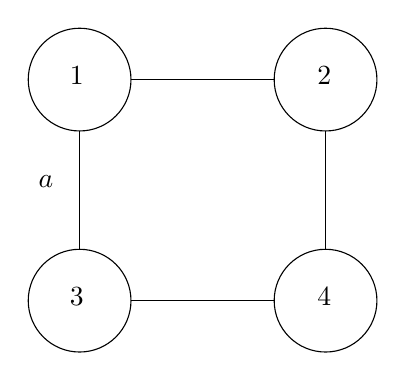
\begin{tikzpicture}[x=0.75pt,y=0.75pt,yscale=-1.5,xscale=1.5]
	\draw   (183.5,100) .. controls (183.5,90.89) and (190.89,83.5) .. (200,83.5) .. controls (209.11,83.5) and (216.5,90.89) .. (216.5,100) .. controls (216.5,109.11) and (209.11,116.5) .. (200,116.5) .. controls (190.89,116.5) and (183.5,109.11) .. (183.5,100) -- cycle ;
	\draw   (183.5,171) .. controls (183.5,161.89) and (190.89,154.5) .. (200,154.5) .. controls (209.11,154.5) and (216.5,161.89) .. (216.5,171) .. controls (216.5,180.11) and (209.11,187.5) .. (200,187.5) .. controls (190.89,187.5) and (183.5,180.11) .. (183.5,171) -- cycle ;
	\draw   (262.5,100) .. controls (262.5,90.89) and (269.89,83.5) .. (279,83.5) .. controls (288.11,83.5) and (295.5,90.89) .. (295.5,100) .. controls (295.5,109.11) and (288.11,116.5) .. (279,116.5) .. controls (269.89,116.5) and (262.5,109.11) .. (262.5,100) -- cycle ;
	\draw   (262.5,171) .. controls (262.5,161.89) and (269.89,154.5) .. (279,154.5) .. controls (288.11,154.5) and (295.5,161.89) .. (295.5,171) .. controls (295.5,180.11) and (288.11,187.5) .. (279,187.5) .. controls (269.89,187.5) and (262.5,180.11) .. (262.5,171) -- cycle ;
	\draw    (216.5,100) -- (262.5,100) ;
	\draw    (200,154.5) -- (200,116.5) ;
	\draw    (262.5,171) -- (216.5,171) ;
	\draw    (279,116.5) -- (279,154.5) ;
	\draw (186,130) node [anchor=north west][inner sep=0.75pt]    {$a$};
	\draw (196,95) node [anchor=north west][inner sep=0.75pt]    {$1$};
	\draw (275.5,95) node [anchor=north west][inner sep=0.75pt]    {$2$};
	\draw (196,166) node [anchor=north west][inner sep=0.75pt]    {$3$};
	\draw (275.5,166) node [anchor=north west][inner sep=0.75pt]    {$4$};
	\end{tikzpicture}
	\caption{Example~\ref{electricpotentialenergyex1}}
\end{figure}
\begin{solution}
	To calculate the potential energy of the entire system, we can calculate it one charge at a time--that is, what energy does adding each charge, one at a time, create? At the beginning, bringing in charge 1 yields 0 energy, since there is no force. Adding charge 2 from the left gives us $U_{E2} = kq_1q_2/a = kq^2/a$. For charge 3, we again have work being done, but by both charge 1 and charge to. Then, we have
	\[U_{E3-1} = k\frac{q^2}{a}\]
	and \[U_{E3-2} = k\frac{q^2}{a\sqrt 2},\] since the distance between 3 and 2 is $a\sqrt 2$. The last charge gives three components, two of which have magnitude $kq^2/a$ (4-3 and 4-2). $U_{E4-1}$ is $kq^2/(a\sqrt 2),$ so we have
	\[\Sigma U_E = 4k\frac{q^2}{a} + 2k\frac{q^2}{a\sqrt 2},\]
	and we're done. 
\end{solution}
\subsection{Conservation of Energy in Electric Systems}
Since electric force is conservative, we know that mechanical energy is conserved in electric systems.
\begin{example}
	Two electrons are held in place, their centers one centimeter apart. They are released and begin flying in opposite directions. How fast is each one moving when they are 10 cm apart? Then, describe their motion as they continue to fly apart.
\end{example}
\begin{solution}
	We know that most of the energy is initially potential. Afterwards, 90\% of the energy is kinetic, since only 10\% of it is potential. We set up a conservation of energy equation such that
	\begin{align*}
		E_{0} &= E_f \\
		U_{0} + K_{0} &= U_{f} + K_f.
	\end{align*}
	Solving for $K_f$ and substituting $K_0 = 0$ yields \[K_f = U_0 - U_f.\] Then, we have
	\begin{align*}
		2\p{\frac{1}{2}mv_f^2} &= k\frac{q_1q_2}{r_0} - k\frac{q_1q_2}{r_f} \\
		mv_f^2 &= kq_1q_2\p{\frac{1}{r_0} - \frac{1}{r_f}} \\
		v_f &= \sqrt{\frac{kq_1q_2}{m}\p{\frac{1}{r_0} - \frac{1}{r_f}}}, 	
	\end{align*}
	so $v_f = \boxed{150\unt{m/s}}$. Now, recall that
	\[a = \frac{\Sigma F}{m}.\]
	Since $F \propto \frac{1}{r^2},$ we know that $a$ will asymptotically approach 0. Velocity will therefore increase, but at a slower rate of time.
\end{solution}

\section{Electric Potential}
In this section, we define electric potential, and examine potential, energy, and work in electric fields.
\subsection{Electric and Potential Field}
Let's begin first with a review of vocabulary. Electric potential is measured in volts, or Joules/Coulomb. This is the same as potential, potential difference, and difference, but not as \textit{energy}. Recall that a charged particle creates an electric field. In fact, particles create another field called the \textit{potential field}.
\begin{defn}[Electric Potential]
    The potential is the amount of potential energy, per unit charge, that a charged object would feel at a location.
\end{defn}
Electric potential is also a scalar. Just like gravitational potential, electric potential is always a \textit{comparison} to the electric potential at another location, such that the potential is zero at infinity. We have two formulas for electric potential:
\begin{equation}
    V = - \int \vec{E}\,\dd \vec{r}
\end{equation}
and
\begin{equation}
    V = \frac{1}{4\pi\eps_0}\sum_i \frac{q_i}{r_i}.
\end{equation}
Suppose we place a charge at a point in space. Recall that an electric field will point away from positive charges and towards negative charges. We can simulate this using a three dimensional surface, such that the potential increases with the $z$-axis. You can see this in the figure below, which graphs surface potential against position (in the $x$-$y$ plane). Note that as we near the positive charge, the potential increases, while as we approach the negative charge it becomes negative.

\begin{figure}[H]
    \centering
    \includegraphics[width=0.8\textwidth]{dipole_ex_potential.png}
    \caption{Dipole Surface Potential}
\end{figure}

Analogically, we treat potential as ``height". We can place a point on the plane, and observe that there is a circle containing this point such that each point on the circle has the same potential.

\begin{example}[AP 2016]\label{potentialex1}
    Examine the equipotential diagram below.
    \begin{enumerate}\setlength\itemsep{0pt}
        \item At point C, draw a vector representing the direction of the electric field at that point.
        \item A proton is placed at point A and then released from rest. Calculate the work done by the electric field on the proton as it moves from point A to point E.
        \item An electron is released from rest at point B. In which direction does it accelerate?
    \end{enumerate}
\end{example}

\begin{solution}
    The electric field must be perpendicular to the equipotential lines, so we place it perpendicular at point C. For part (2), we know
    \begin{align*}
        W &= -\Delta U_E \\
        W &= -q\Delta V \\
        W &= -q(V_f - V_0),
    \end{align*}
    so $W = \boxed{1.28\times 10^{-18}\unt{J}}$. We know that positive charges aim to go to lower potential, whereas negative charges go to higher potentials. Therefore, it accelerates left towards $q_2$, increasing potential.
\end{solution}
\begin{figure}[H]
    \centering
    \includegraphics[width=0.8\textwidth]{ap_potential_ex.png}
    \caption{Example~\ref{potentialex1}}
\end{figure}
\subsection{Work and Change in Potential}
Here, we're going to work on moving a charge in an electric field. Suppose that a positive charge at the origin generates an electric field. Another positive charge is placed at point A in the first quadrant, and is moved to the right to point B. We can describe its change in position vector, $\vb{r}$, as two components, one parallel and one perpendicular to the field. The perpendicular component yields $\Delta V = 0$. The parallel component shows that the particle moves from a region of higher to lower potential as it moves further away from the field, so $\Delta V < 0$.

Now suppose it moves to a point C up and to the right. Again, we split this into perpendicular and parallel components, giving us $\Delta V_{\perp} = 0$ and $\Delta V_{\parallel} < 0$. Finally, suppose it moves back to the same location. Then, there is no $\Delta V$.

We can summarize this as follows.
\begin{enumerate}\setlength\itemsep{0pt}
    \item Electric field lines point to a lower potential
    \item Positive charges lose potential energy when they move to a lower potential
    \item Movement perpendicular to the field involves no work and no $\Delta V$
    \item Since $\vb{F}_E$ is conservative, any closed path requires no work or $\Delta V$
\end{enumerate}
\begin{example}\label{potentialex2}
    Consider the electric field diagram above.
    \begin{enumerate}\setlength\itemsep{0em}
        \item At which of these four points is the magnitude of the electric field the greatest?
        \item At which of these four points is the electric potential the greatest?
        \item An electron is released from rest at point $B$. Describe the electron's motion in terms of direction, speed, and acceleration.
    \end{enumerate}
\end{example}
\begin{solution}
    Note first that this is not an equipotential diagram, but a field diagram. When the field lines are closest together, the magnitude of the field is greatest, so we find that $\max |\vb{E}|$ is found at $\boxed{C}$. We know that electric field points to lower potential, so $\max V$ is at $\boxed{A}$. The electron at point $B$ is negatively charged, so it will accelerate to the left (and it's speed will increase).
\end{solution}
\begin{figure}
    \centering
    \includegraphics[width = 0.8\textwidth]{electric_potential_ex3.png}
    \caption{Example~\ref{potentialex2}}
\end{figure}
\subsection{Electric Field vs. Electric Potential}
Here, we're going to look at the differences between electric field and potential. Note the following formula, which describes electric field in terms of potential
\[\vec{E}_x = -\dv{V}{x}.\]
Observe that this is not a time derivative, but a space derivative. Just as we draw analogy between height and potential, we can likewise derive an analogy between steepness and electric field (i.e. slope).
\begin{example}\label{potentialex3}
    Five different charge configurations on the $x-y$ plane, each using two or four point charges of equal magnitude, are shown in the figure. All charges are the same distance from the origin. The electric potential infinitely far from the origin is defined to be zero.
    \begin{enumerate}
        \item In which configuration are both the electric field and the electric potential equal to zero at the origin?
        \item In which configuration is the electric field zero at the origin, but not the electric potential?
    \end{enumerate}
\end{example}
\begin{solution}
    We know that field is zero when there is no net force. Clearly, $A, B$ and $C$ have a net force. However, in $D$ and $E$, the electric field is zero, as $\Sigma \vb{F} = 0$. The potential is given by
    \[V = k\frac{q}{r},\]
    so since the charges in $D$ are all the same, $V \neq 0$. Thus, we have that $\vb{E}$ and $V$ are zero at the origin in $\boxed{E}$. For question 2, we then have $\boxed{D}$.
\end{solution}
\begin{figure}
    \centering
    \includegraphics[width = 0.8\textwidth]{electric_potential_ex4.png}
    \caption{Example~\ref{potentialex3}}
\end{figure}

\begin{example}
    Six particles, each with charge $+Q$, are held fixed and equally spaced around the circumference of a circle of radius $R$. What is the magnitude of the resultant electric field at the center? How much work would be done by an external force to bring a seventh particle of charge $+Q$ from very far away and place it at the center of the circle?
\end{example}
\begin{solution}
    Trivially by symmetry we find that $\vb{E} = \boxed{0}$. Next, we know that
    \[W_{ex} = \Delta U,\]
    so we can then use $U = q\Delta V$. Since $V_f = 6kQ/R$, we have
    \begin{align*}
        W_{ex} &= q\Delta V \\
        &= q\left(V_f - V_0\right) \\
        &= Q\p{6k\frac{Q}{R}-0} \\
        &= 6k\frac{Q^2}{R},
    \end{align*}
    and we're done.
\end{solution}

\subsection{Field and Potential of Continuous Charge Distributions}
Here, we'll look at the field and potential of a continuous charge distribution, in the shape of a semi-circle. Recall the equations for electric field and electric potential. We can differentiate with respect to charge, giving us
\begin{equation}
    \dd \vec{E} = \frac{k\dd q}{r^2} \vu{r}
\end{equation}
for field, and
\begin{equation}
    \dd V = \frac{k\dd q}{r}
\end{equation}
for potential. These effectively tell us the small difference in field/potential given by a small sub-charge. Also consider that the semi-circle is uniformly charged, meaning that $\lambda$ is constant throughout.
\begin{example}
    A quarter circle of radius $R$ is uniformly charged with total charge $Q$. What are the electric field and electric potential at the origin?
\end{example}
\begin{solution}
    Note that each $\dd q \in Q$ will create a small vector $\dd\vec{E}$ pointing outwards. Observe that from symmetry, $\vec{E}_y = 0$. Then, $\Sigma \vec{E} = \vec{E}$. For each $\dd q$, we can create a small $\vu{r}$, such that $\vu{r}$ is the hypotenuse of a right triangle. We can write
    \[\dd\vec{E} = \frac{k\dd q}{r^2}(-\cos\theta \vu{\imath} - \sint\vu{\jmath}),\]
    where $\theta$ is the angle from the $x$-axis to $\vu{r}$. Then, we integrate, such that
    \begin{align*}
        \vec{E}_x &= \int \frac{k\dd q}{R^2}(-\cost).    
    \end{align*}
    Of course we also need to have bounds on our integral. Using $\theta$ from the $x$-acis, we have $\theta_0 = \frac{3\pi}{4}$ and $\theta_0 = \frac{5\pi}{4}$. Then, we have
    \begin{align*}
        \vec{E}_x &= \frac{k}{R^2} \int_{3\pi/4}^{5\pi/4} \dd q (-\cost).
    \end{align*}
    Since $\lambda$ is constant, we have
    \[\lambda = \frac{4Q}{2\pi R} = \frac{\dd q}{\dd l}\]
    where $\dd l$ is the length of $\dd q$. Then, from the equation for arc length, we know $\dd l = \dd\theta R$. Writing our integral out again gives us
    \begin{align*}
        \vec{E}_x &= \frac{k}{R}\lambda\int_{3\pi/4}^{5\pi/4} -\cost\dd \theta \\
        &= \frac{k\lambda}{R}\p{-\sint\Big|_{3\pi/4}^{5\pi/4}} \\
        &= \frac{\sqrt{2} k\lambda}{R} \\
        &= \boxed{\frac{2\sqrt{2}kQ}{\pi R^2}}.
    \end{align*}
    For electric potential, consider the formula for $\dd V$. Integrating gives us
    \[V = \int_{3\pi/4}^{5\pi/4} \frac{k}{R}\dd q.\]
    Using the same substitution with $\lambda$ as above, we have
    \begin{align*}
        V &= k\lambda\int_{3\pi/4}^{5\pi/4} \dd \theta \\
        &= k\lambda\p{\frac{\pi}{2}} \\
        &= \boxed{\frac{kQ}{R}},    
    \end{align*}
    and we're done.
\end{solution}

\newpage
\part{Conductors and Capacitors}
This unit focuses on more advanced electrostatics, like conductors and capacitors. It covers unit 2 in the AP Physics C: E\&M Course and Exam Description.
\section{Electric Fields of Conductors}
In this section, we define conductors and examine their properties, specifically in regards to electric field and electric potential.
\subsection{Excess Charges on Conductors}
Any excess charge on an isolated conductor will spread over it's surface until there is no more charge movement. This is called \textit{electrostatic equilibrium}.

\begin{table}[H]
    \centering
    \begin{tabular}{lcl}
        \toprule
        & Location & Attributes \\ \midrule
        \multirow{2}{*}{Electric Field} & Inside & 0 \\
        & Surface & Perpendicular \\
        \multirow{2}{*}{Electric Potential} & Inside & Equal to $V_{\text{surface}}$ \\
        & Outside & Constant \\ \bottomrule
    \end{tabular}
    \caption{Properties of Objects in Electrostatic Equilibrium}
\end{table}

Earlier, we looked at electric field in space for single and double point charges in space. Here, we'll look at fields inside \textit{conductors}.
\begin{defn}[Conductors]
    Conductors are materials which have many free electrons.
\end{defn}
Suppose we have positive charge placed on a conductor. In this case, the charge is free to move around the conductor. However, in placing a second positive charge, the second charge is now exactly opposite the first. We can generalize this to $n$ charges, saying that the charges $q_1, q_2\dots q_n$ will maximize the distance between each other, becoming equidistant.
\begin{law}
    Excess charges will move as far apart as possible until the system is in electrostatic equilibrium.    
\end{law}
The ideas from above can be explained in terms of this principle. For example, if the electric field inside the conductor were not 0, electrons would accelerate and the object would not be in equilibrium. We can summarize this graphically as the following:
\begin{figure}[H]
    \centering
    \includegraphics[width=\textwidth]{phy_conductor_graph_1.png}
\end{figure}

Consider, now, irregularly shaped conductors. Unlike shperical ones, the electric field will not be symmetric, but the electric potential inside the conductor will always be equal to the surface potential. Note that since electric field is perpendicular to the surface, the field will be greatest when the surface curves the most.
\begin{question}
    Why is $\vec{E}$ perpendicular to the surface?    
\end{question}
Suppose that $\vec{E}$ wasn't perpendicular. Then, there would be a force on the free electrons, meaning that they would accelerate--and therefore, not be in equilibrium.
\begin{example}
    Two conducting spheres, one having twice the diameter of the other, are shown above. The smaller sphere initially has a charge $+q$. When the spheres are connected by a thin wire, which of the following is true?
    \begin{enumerate}[noitemsep, label=(\alph*)]
        \item 1 and 2 are both at the same potential
        \item 2 has twice the potential of 1
        \item 2 has half the potential of 1
        \item 1 and 2 have equal charges
        \item All of the charge is dissapated
    \end{enumerate}
\end{example}
\begin{solution}
    Note that since these are conductors, the potential must be the same everywhere. We then obviously have $\boxed{(a)}$.   
\end{solution}
\begin{example}
    Which of the following statements about conductors under electrostatic conditions is true?
    \begin{enumerate}[noitemsep, label=(\alph*)]
        \item Positive work is required to move a positive charge over the surface of a conductor
        \item Charge that is placed on the surface of a conductor always spreads evenly over the surface
        \item The electric potential inside a conductor is always zero
        \item The electric field at the surface of a conductor is tangent to the surface
        \item The surface of a conductor is always equipotential
    \end{enumerate}
\end{example}
\begin{solution}
    First note that (b) must be false, as the surface is not necessarily spherical. However, (e) must be true no matter what.
\end{solution}
\subsection{Spherical Conducting Shells}
Recall that
\[V = k\frac{Q}{r},\]
and that
\[q\Delta V = \Delta U.\]
\begin{example}[AP 1990]
    A sphere of radius $R$ is surrounded by a concentric spherical shell of inner radius 2R and outer radius $3R$. The inner sphere is an insulator containing a net charge + Q distributed uniformly throughout its volume. The spherical shell is a conductor containing a net charge $+q$ different from $+Q$. Given the electric fields in the table below, find the potential as a function of distance $x$ from the center
    \begin{enumerate}[noitemsep , label=(\alph*)]
        \item outside the conducting shell ($r>3R$)
        \item within the shell ($2R < r < 3R$)
        \item between the outer shell and the inner shpere
    \end{enumerate}
\end{example}
\begin{table}[H]
    \centering
    \begin{tabular}{cc}
        \toprule
        Domain & Electric Field \\ \midrule
        $r < R$ & $\sfrac{kQr}{R^3}$ \\
        $R < r < 2R$ & $\sfrac{kQ}{r^2}$ \\
        $2R < r < 3R$ & 0 \\
        $r > 3R$ & $\sfrac{k(Q+q)}{r^2}$ \\ \bottomrule
    \end{tabular}    
\end{table}
\begin{solution}
    We start with setup. We use the formula
    \[\Delta V = -\int_a^b\vec{E}\cdot\dd\vec{r}.\]
    The potential for $x > 3R$ is given by the improper integral below, where we set $a = \infty$:
    \begin{align*}
        V_{x > 3R} &= -\int_{\infty}^{x} \vec{E}\cdot\dd \vec{r} \\
        &= -\int_{\infty}^{x}\frac{k(Q+q)}{r^2}\,\dd r\\
        &= -k(Q+q) \int_{\infty}^{x} \frac{\dd r}{r^2} \\
        &= -k(Q+q)\p{-\frac{1}{r}\Big|_{\infty}^x}.
    \end{align*}
    From the definition of an improper integral, we then have
    \begin{align*}
        V_{x>3R} &= k(Q+q)\p{\frac{1}{x}-\lim_{x\to\infty}\frac{1}{x}} \\
        &= \frac{k(Q+q)}{x}  
    \end{align*}
    Observe that this is simply the same as if it was a point charge, since $q_{tot} = Q+q$. For $V_{2R-3R}$, we have
    \begin{align*}
        V_{2R<x<3R} &= -\p{\int_{\infty}^{3R} \vec{E}\cdot\dd\vec{r}+ \int_{3R}^{x} \vec{E}\cdot\dd\vec{r}}.
    \end{align*}
    However, observe that the second integral simply evaluates to 0. Thus, we again have
    \[V_{2R<r<3R} = \frac{k(Q+q)}{3R}.\]
    For the final component, we have
    \begin{align*}
        V &= -\p{\int_{\infty}^{2R}\vec{E}\cdot \dd r + \int_{2R}^x\vec{E}\cdot\dd r}.    
    \end{align*}
    Subsituing our value of $V_{2R<r<3R}$ from above into the first integral yields
    \begin{align*}
        V &= \frac{k(Q+q)}{3R} - \int_{2R}^x \vec{E}\cdot \dd r \\
        &= \frac{k(Q+q)}{3R} - \int_{2R}^x \frac{kQ}{r^2}\cdot \dd r \\
        &= \frac{k(Q+q)}{3R} - kQ\p{\frac{1}{r}\Big|_{2R}^x} \\
        &= \frac{k(Q+q)}{3R} - kQ\p{\frac{1}{x}-\frac{1}{2R}}.
    \end{align*}
    Also observe that the potential is simply proportional to $1/x$, up to a constant.
\end{solution}
\subsection{Concentric Shells}
Here, we look at electric fields and concentric shells, and also discuss electrostatic shielding. Observe the diagram below, which describes two plates charged with a battery.
\begin{figure}[H]
    \centering
    \includegraphics[width=0.7\textwidth]{phy_electric_shielding_1.png}
\end{figure}

Now suppose we place an insulating material inside this field. The electric field will go directly through the insulator, as there is no shielding. However, if we place a conductor inside, an electric field flowing in the \textit{opposite} direction will flow through it, as below. Therefore, the field will be zero, since it will cancel out. This is called electric shielding.
\begin{figure}[H]
    \centering
    \includegraphics[width=0.7\textwidth]{phy_electric_shielding_2.png}
\end{figure}
\begin{example}[AP 1988]
    An isolated conducting solid sphere of radius $a$ is charged to potential $V$. Determine the charge on the sphere.
\end{example}
\begin{solution}
    Using Gauss's law, we have
    \[E = \frac{kQ}{r^2}\]
    and \[V = \frac{kQ}{r}\] outside the conductor, and $E = 0$ and \[V = \frac{kQ}{a}\] inside. We then have, inside the conductor, \[Q = \frac{Va}{k},\]
    and we're done.
\end{solution}
\begin{example}
    Two conducting hemispherical shells of inner radius $b$ are brought up, and, without contacting a solid sphere of radius $a$, are connected to form a spherical shell surrounding and concentric to the solid sphere. The outer shell is then grounded. Determine the potential of the solid sphere, relative to ground.
\end{example}
\begin{solution}
    Recall that grounds are an \textit{infinite} source or sink for electrons, such that a grounded positively charged object will gain electrons to become neutral, and a grounded negative object will lose them. Here, we need to find potential relative to the ground, so we have
    \begin{align*}
        \Delta V &= -\int_b^a\vec{E}\cdot\dd r \\
        &= -\int_{b}^a k\frac{Q}{r^2}\dd r \\
        &= -kQ\int_b^a \frac{1}{r^2} \dd r \\
        &= kQ\p{\frac{1}{r}\Big|_{b}^a} \\
        &= kQ\p{\frac{1}{a}-\frac{1}{b}}.
    \end{align*}
    Substituting from above with $Q$, we have
    \[\Delta V = V\p{1-\frac{a}{b}},\]
    and we're done.
\end{solution}
\subsection{Two Charged Conductors}
Here, we'll look at the behavior of charges as systems move towards equilibrium.
\begin{example}[Two Spherical Conductors Problem]
    An isolated spherical conductor of radius $r_a$ has a charge $Q$. A second isolated spherical conductor of radius $r_b = 0.5r_a$ has no net charge. They are then connected by a conducting wire, and the system comes to equilibrium. Find the ratio of surface charge densities on sphere $a$ and sphere $b$.
\end{example}
\begin{solution}
    Note that in essence, this system is just a simple conductor. Then, the surface and interior of this conductor have equal potentials. The surface charge density $\sigma$ is given by the total charge divided by surface area, so we have
    \begin{align*}
        \frac{\sigma_a}{\sigma_b} &= \frac{\frac{Q}{4\pi r_a^2}}{\frac{q_b}{4\pi r_b^2}} \\
        &= \frac{Q}{q_b} \cdot \frac{r_b^2}{r_a^2} \\
        &= \frac{Q}{4q_b}.
    \end{align*}
    Essentially, we need to find an expression for $q_b$ in terms of $Q$. We set the surface potentials equal, giving us
    \begin{align*}
        V_a &= V_b \\
        \frac{kQ}{r_a} &= \frac{kq_b}{r_b}.
    \end{align*}
    We then find that the ratio $Q/q_b$ is given by $r_a/r_b = 2$. Thus, we have $\sigma_a/\sigma_b = 2/4 = 1/2$.
\end{solution}
\begin{example}
    Two conducting spheres of different radii each have charge $-Q$. Which of the following occurs when the two spheres are connected with a conducting wire?
    \begin{enumerate}[noitemsep, label=(\alph*)]
        \item No charge flows
        \item Negative charge flows from the larger sphere to the smaller sphere until they have equal electric fields at their surface
        \item Negative charge flows from the larger sphere to the smaller sphere until they have equal electric potentials at their surface
        \item Negative charge flows from the smaller sphere to the larger sphere until they have equal electric fields at their surface
        \item Negative charge flows from the smaller sphere to the larger sphere until they have equal electric potentials at their surface
    \end{enumerate}
\end{example}
\begin{solution}
    We know that \[V_{S} = V_{L}.\] We know that the potentials must be the same, and we also know that
    \[-\frac{kQ}{r_S} = -\frac{kQ}{r_L}.\]
    Given that $r_L > r_S$, we must then have a smaller $q_s$ at the end in order to balance the equation. Thus, we have that the charge flows from small to large, or (e).
\end{solution}
\section{Parallel Plate Capacitors}
We define a capacitor as a device that can store and transform electric potential energy. An example of a simple capacitor is a system of two plates, each with area $A$, separated by distance $d$. We can assume that $A >> d$. When we connect a capacitor to a battery, as below, the capacitor will be at a lower potential than the battery.
\begin{figure}[H]
    \centering
    \begin{tikzpicture}[x=0.75pt,y=0.75pt,yscale=-1,xscale=1]
        \draw   (269,242) -- (305,242) (313,212) -- (313,272) (313,242) -- (349,242) (301.8,227) -- (305,227) -- (305,257) -- (301.8,257) -- (301.8,227) -- cycle ;
        %Straight Lines [id:da7577343216505839] 
        \draw    (160,242) -- (269,242) ;
        %Straight Lines [id:da9565697791571119] 
        \draw    (349,242) -- (460,242) ;
        %Straight Lines [id:da10543744665189592] 
        \draw    (160,242) -- (160,115) ;
        %Straight Lines [id:da8583665956500706] 
        \draw    (160,115) -- (218,115) ;
        %Straight Lines [id:da32905308642854303] 
        \draw    (460,242) -- (460,115) ;
        %Straight Lines [id:da2761066049341392] 
        \draw    (370,115) -- (460,115) ;
        %Shape: Square [id:dp4484580435451402] 
        \draw   (282,139.32) -- (282,75.31) -- (218,90.68) -- (218,154.69) -- cycle ;
        %Shape: Square [id:dp3631393363273352] 
        \draw   (402,139.32) -- (402,75.31) -- (338,90.68) -- (338,154.69) -- cycle ;
        %Straight Lines [id:da6664850395263688] 
        \draw  [dash pattern={on 4.5pt off 4.5pt}]  (218,115) -- (250,115) ;
        % Text Node
        \draw (384,83.4) node [anchor=north west][inner sep=0.75pt]    {$-$};
        % Text Node
        \draw (264,83.4) node [anchor=north west][inner sep=0.75pt]    {$+$};
        % Text Node
        \draw (240,59.4) node [anchor=north west][inner sep=0.75pt]    {$Q$};
    \end{tikzpicture}
    \caption{Capacitor}
\end{figure}

This potential difference drives charges into the capacitor, so that it eventually becomes fully charged when the potential of the battery is equal to that of the plates. We then say that each plate has charge magnitude $|Q|$.
\begin{question}
    Where do the charges that initially move into the plates come from?    
\end{question}
We can find that
\[Q \propto \Delta V,\]
since as the potential difference increases, the charge does as well. We can say that they are proportional up to a constant $C$, such that
\[Q = C\Delta V.\]
This $C$ is called \textit{capacitance}, and is also given by
\begin{eqn}[Capacitance with Charge]
    For a capacitor with charge $Q$ and capacitance $C$,
    \begin{equation}
        \Delta V = \frac{Q}{C}.
    \end{equation}
\end{eqn}
Capacitance is measured in $C/V$, which is equal to a \textit{Farad}, or $F$. We can also consider the capacitance proportional to area, and inversely proportional to distance. We then have
\[C \propto \frac{A}{d},\]
which can be expressed as
\begin{equation}
    C = \frac{A\eps_0}{d}.
\end{equation}
Suppose, however, that the plates are of unequal area. Instead, we have a dielectric (insulator) which fills the space between the plates, giving us
\[C = \frac{A\eps}{d},\]
where $\eps$ is defined as the \textit{permittivity of the medium}, and depends on the dielectric between the plates. We define a constant $\kappa$ as the \textit{dielectric constant}, and is given by
\[\kappa = \frac{\eps}{\eps_0}.\]
In a vacuum, $\kappa_{\text{vacuum}} = 1$. $\kappa$ depends on the medium, but we can use it to find our final expression for capacitance,
\begin{eqn}[Capacitance with Area]
    For a dielectric with constant $\kappa$, the capacitance $C$ of a capacitor with area $A$ and distance $d$ is
    \begin{equation}
        C = \frac{\kappa\eps_0A}{d}.
    \end{equation}
\end{eqn}
Using our two expressions for capacitance, we can then derive
\begin{equation}
    \frac{Q}{\Delta V} = \frac{\kappa\eps_0 A}{d}.
\end{equation}
\begin{example}
    A dielectric is inserted into a parallel plate capacitor connected to a battery. If the dielectric completely fills the space between the plates, what changes, if any, occur to $\kappa$, $Q$, or $\Delta V$?
\end{example}
\begin{solution}
    We know, from above, that
    \[\frac{Q}{\Delta V} = \frac{\kappa\eps_0 A}{d}.\]
    Note that $A$, $d$, $\eps_0$, and $\Delta V$ all remain constant. Since $\kappa$ increases, we then must have an increase in charge $Q$ on the left hand side.
\end{solution}
\begin{example}
    A dielectric is inserted into a parallel plate capacitor connected to an isolated charged capacitor. If the dielectric completely fills the space between the plates, what changes, if any, occur to $\kappa$, $Q$, or $\Delta V$?
\end{example}
\begin{solution}
    Here again, $\kappa$ increases. However, $Q$ must be constant, meaning that $\Delta V$ must decrease in turn.
\end{solution}
Now, we'll study capacitors from a more rigorous mathematical perspective. Recall that in a charged sheet, we have
\[|E| = \frac{\sigma}{2\eps_0}.\]
For determining the capacitance equation, the process is similar. We must first apply Gauss's law in integral form, and determine the electric field. We can then use
\[\Delta V = -\int \vb{E} \cdot \dd\vb{r}\]
to determine the potential difference, and then solve for capacitance with $Q = C\Delta V$. We start with a parallel plate capacitor, such that each plate has area $a$ and charge $|Q|$ (the top plate is positive and the bottom is negative), and is separated by distance $d$. We then know that
\[\oint \vb{E}\cdot\dd\vb{A} = \frac{Q}{\eps_0}.\]
Splitting this surface integral into three components yields
\[\oint_{\text{top}} \vb{E}\cdot\dd\vb{A} + \oint_{\text{sides}} \vb{E}\cdot\dd\vb{A} + \oint_{\text{bottom}} \vb{E}\cdot\dd\vb{A}= \frac{Q}{\eps_0}.\]
Since $\theta_{\text{side}} = 90\degr$, and $\vb{E}_{\text{top}} = 0$, we then simply have
\[\oint_{\text{bottom}} \vb{E}\,\dd\vb{A} = \frac{Q}{\eps_0}.\]
We then simplify to get
\[E = \frac{Q}{A\eps_0}.\]
Substituting into the $\Delta V$ integral yields an angle of $\theta = 180\degr$, so we have
\[\Delta V = \frac{Q}{A\eps_0} \int_0^d \dd\vb{r},\]
which is equivalent to $\frac{Qd}{A\eps_0}$. With the capacitance equation, we thus have
\begin{align*}
    \Delta V &= \frac{Q}{C} \\
    \frac{Qd}{A\eps_0} &= \frac{Q}{C} \\
    C &= \boxed{\frac{A\eps_0}{d}}.
\end{align*}
Next, supposed we have two cylindrical conductors, one with outer radius $b$ and the other of radius $a$, such that the outer one has charge $-Q$ and the inner one is of charge $+Q$. Applying Gauss's law yields
\[\oint \vb{E}\cdot\dd\vb{A} = \frac{Q}{\eps_0}.\]
Note, however, that the angle $\theta = 90\degr$ for the caps of the cylinders, thus giving us
\begin{align*}
    \vb{E}\oint \dd\vb{A} &= \frac{Q}{\eps_0} \\
    E(2\pi r\ell) &= \frac{Q\ell}{\eps_0 L} \\
    E &= \frac{Q}{2\pi\eps_0 Lr}.
\end{align*}
Integrating with respect to $\vb{r}$ gives us
\begin{align*}
    \Delta V &= -\int_b^a \frac{Q}{2\pi\eps_0 Lr} \cdot\dd\vb{r} \\
    &= -\frac{Q}{2\pi\eps_0 L} \p{\ln(r)\Big|_b^a} \\
    &= \frac{Q}{2\pi\eps_0 L} \ln\p{\frac{b}{a}}.    
\end{align*}
We thus have
\[C = \boxed{\frac{2\pi\eps_0 L}{\ln\p{\frac{b}{a}}}}.\]
\section{Energy Stored In Capacitors}
Here, we'll cover the energy stored in capacitors, as well as the energy density of an electric field.
\begin{question}
    What will happen after the charged capacitor is connected to the bulb in the figure below?
\end{question}
In particular, observe the brightness of the bulb, the stored energy, the charges, and the field lines.

\begin{figure}[H]
    \centering
    \includegraphics[width = 0.6\textwidth]{energy_in_capacitor_ex1.png}
\end{figure}

When the capacitor is connected, the brightness of the bulb, electric field lines, and stored energy decrease. Observe that the work done can be written as
\[\dd W = \dd U = V'\dd q,\]
where $V'$ is the potential difference. We then have
\[U_C = \int_0^{Q} V'\,\dd q.\]
We can also substitute with $Q/C = \Delta V$, giving us
\begin{align*}
    U_C &= \int_0^Q \frac{q}{C}\,\dd q \\
    &= \frac{1}{2C}\p{q^2\Big|_0^Q},    
\end{align*}
so we have
\begin{eqn}[Energy of a Capacitor]
    The energy in a capacitor with potential difference $\Delta V$, charge $Q$, and capacitance $C$ is
    \begin{equation}
        U_C = \frac{1}{2}Q\Delta V = \frac{1}{2} C(\Delta V)^2.
    \end{equation}
\end{eqn}
Next, we'll derive an equation for energy density in a field. Recall that
\[C_0 = \frac{\eps_0 A}{D},\]
and \[E_x = -\dv{V}{x}.\] We can instead state that $|E| = \frac{\Delta V}{d},$ since electric field is constant between the plates. We thus have
\[U_C = \frac{Q(\Delta V)^2}{2}.\]
Note that this is also equivalent to our expression for the energy of the capacitor. We can also substitute $C(\Delta V)^2$ giving us
\[U_C = \frac{\eps_0 AE^2d^2}{2d},\]
or \[U_C = \frac{\eps_0 E^2 Ad}{2}.\]
Dividing by volume to find the \textit{energy density} gives
\[u_E = \frac{\eps_0 E^2}{2}.\]
Note also that $u_E \propto E^2$.
\subsection{Practice Problems}
Consider the following questions.
\begin{example}[1981 AP E1]
    A conducting sphere of radius $a$ and charge $Q$ is surrounded by a concentric conducting shell of inner radius $b$ and outer radius $c$ as shown. The outer shell is first grounded, and the grounding wire is then removed.
    \begin{enumerate}[label=(\alph*)]
        \item Using Gauss's law, determine the electric field in the region $a < r < b$, where $r$ is the distance from the center of the inner sphere.
        \item Develop an expression for the capacitance $C_0$ of the system of spheres.
    \end{enumerate}
\end{example}
\begin{solution}
    First notice that after grounding and removing the wire from the outer shell, the shell will then have a net negative charge of magnitude $Q$. We then use Gauss's law with a Gaussian sphere to determine the electric field. Note that $q_{enc} = Q$, so we have
    \begin{align*}
        \oint \vb{E}\cdot\dd\vb{A} &= \frac{q_{enc}}{\eps_0} \\
        E(4\pi r^2) &= \frac{Q}{\eps_0} \\
        E &= \boxed{\frac{kQ}{r^2}},
    \end{align*}
    the same as a point charge. To determine the capacitance, we integrate electric field with respect to $\vb{r}$, so we have
    \begin{align*}
        \Delta V &= -\int \vb{E}\cdot \dd\vb{r} \\
        &= \int_a^b \frac{kQ}{r^2}\,\dd\vb{r} \\
        &= kq\int_a^b \frac{1}{r^2}\,\dd r \\
        &= kq\p{-\frac{1}{r}\Big|_a^b} \\
        &= \frac{kq(b-a)}{ab}.
    \end{align*}
    Then, using the fact that
    \[C = \frac{Q}{\Delta V},\]
    we substitute, giving us
    \[C_0 = \boxed{\frac{ab}{k(b-a)}},\]
    and we're done.
\end{solution}
\begin{example}
    A parallel plate capacitor is connected to a battery of potential difference $V$. If the plate is of area $A$ and the plates are separated by distance $x$, find the attractive force between the plates.    
\end{example}
\begin{solution}
    We can use the fact that
    \[U = \frac{CV^2}{2}\]
    to find an expression for $U$ in terms of $x$ and $A$. As $C = A\eps_0/x,$ we have
    \[U = \frac{\eps_0 AV^2}{2x}.\]
    We also know that $F = -\dv{U}{x}$, so we have
    \[F = \boxed{\frac{\eps_0 AV^2}{2x^2}},\]
    and we're done.
\end{solution}
\begin{example}[1994 AP E2]
    A parallel plate capacitor is made from two sheets of metal, each with an area of 1.0 square meters, separated by a sheet of plastic 1.00 mm thick. The capacitance is measured to be 0.05 microfarad.
    \begin{enumerate}[label=(\alph*)]
        \item What is the dielectric constant of the plastic?
    \end{enumerate}
    After the capacitor is fully charged, it is carefully disconnected, leaving the charged capacitor isolated in space. The plastic sheet is then removed from between the metal plates. The metal plates retain their original separation of 1.0 mm. The original voltage is 30 V.
    \stepcounter{enumi}
    \begin{enumerate}[label=(\alph*), resume]
        \item What is the new voltage across the plates?
        \item If there is now more energy stored in the capacitor, where did it come from? If there is now less energy, what happened to it?
    \end{enumerate}
\end{example}
\begin{solution}
    For part (a), we know that
    \[C= \frac{\kappa\eps_0 A}{d}.\]
    Solving for $\kappa$ yields
    \[\frac{Cd}{\eps_0 A} = \kappa,\]
    so $\kappa = \boxed{5.65}$. For (c), we use the fact that
    \[\frac{Q}{\Delta V} = \frac{\kappa\eps_0 A}{D}.\]
    The charge $Q$ must remain the same, but as $\kappa$ decreases, $\Delta V$ must increase proportionally. We then have $V_f = V_0\cdot\kappa = \boxed{170\unt{V}}.$ In part (d), we note that
    \[U = \frac{Q\Delta V}{2}.\]
    As the energy increases, work is done to pull the dielectric out. This work results in an increase in the potential energy in the capacitor.
\end{solution}
\section{Dielectrics}

Suppose that we have two parallel plate capacitors, one separated by a vacuum and one separated by a dielectric. Recall that the capacitance for the vacuum is given by
\begin{equation}
    C_0 = \frac{\eps_0 A}{d},
\end{equation}
and the equation for the dielectric capacitance is
\begin{equation}
    C = \frac{\kappa \eps_0 A}{d},
\end{equation}
where $\kappa$ is the dielectric constant of the medium. This gives us the additional relationship
\begin{equation}
    C = \kappa C_0.
\end{equation}
Adding a dielectric can very drastically change capacitance. For example, calcium copper titanate ($\ce{CaCu3Ti4O12}$) has a dielectric constant $\kappa > 10,000$. The molecules within dielectrics can be either \textit{polar} or \textit{nonpolar}. Within an electric field, polar molecules will align themselves such that one end is positive and one is negative (with the positive end facing the negative plate, and the negative end facing the positive plate).

The electric field of the dielectric, $\vb{E}_d$, faces the opposite direction of the electric field of the plates, such that \[\Sigma \vb{E} = \vb{E}_0 - \vb{E}_d < E_0.\]
Therefore, adding a dielectric decreases the electric field, thereby increasing the capacitance.
\begin{example}
    An isolated parallel plate capacitor of capacitance $C$ stores a charge $Q$. A slab of dielectric of mass $m$ near the plates is pulled into the capacitor and enters the space with negligible friction. What maximum speed can the slab reach within the capacitor?
\end{example}
\begin{solution}
    We can solve using conservation of energy. Note that
    \[E_0 = E_f,\]
    so then have
    \[U_0 = U_f + K_f,\]
    as $K_0 = 0$. Then, using $U = \frac{Q^2}{2C}$, we have
    \begin{equation*}
        \frac{Q^2}{2C_0} = \frac{Q^2}{2C_f} + \frac{1}{2}mv_f^2.    
    \end{equation*}
    Setting $C_f$ to $\kappa C_0$ yields
    \begin{align*}
        \frac{Q^2}{2C_0}\p{1 - \frac{1}{\kappa}} &= \frac{1}{2}mv_f^2 \\
        v_f &= \sqrt{\frac{Q^2(\kappa -1)}{m\kappa C_0}},
    \end{align*}
    and we're done.
\end{solution}
\subsection{Dielectrics and Energy}
Recall that
\begin{equation}
    \frac{Q_i}{\Delta V} = \frac{\kappa\eps_0 A}{d}.\label{kappaepsq_eq}
\end{equation}
Suppose that we place a dielectric with constant $\kappa$ between two parallel plates. We then can state that
\[U_f = \frac{Q_f\Delta V}{2}.\]
Using Equation~\ref{kappaepsq_eq}, we can then say that
\[Q_f = \kappa Q_i,\]
therefore giving us
\begin{equation}
    U_f = \frac{\kappa Q_i\Delta V}{2}.
\end{equation}
Now suppose we do the same but such that the plates are not connected to the battery. We then have
\[\Delta V_f = \frac{\Delta V_i}{\kappa},\]
now giving us
\begin{equation}
    U_f = \frac{Q\Delta V_i}{2\kappa}.
\end{equation}
\begin{example}
    Initially, a parallel-plate capacitor is connected to a battery of potential difference $V$, and is fully charged. The capacitor is then disconnected and completely submerged in a nonconducting fluid of dielectric fluid with constant $\kappa$. If the area of the plates is $A$ and the distance between them is $d$, derive
    \begin{enumerate}[label=(\alph*)]
        \item the potential difference after the capacitor is submerged.
        \item the difference in energy of the capacitor between the initial and final states.
    \end{enumerate}
\end{example}
\begin{solution}
    Solving for part (a) gives us
    \[V_f = \boxed{\frac{V}{\kappa}},\]
    as above. For part (b), we know that
    \[Q = \frac{V\eps_0 A}{d},\]
    as $\kappa = 1$. We then have that
    \[U_0 = \frac{QV}{2}\]
    and \[U_f = \frac{QV}{2\kappa}.\]
    Then, we can write
    \begin{align*}
        \Delta U &= \frac{QV}{2} - \frac{QV}{2\kappa} \\
        &= \frac{QV}{2}\p{1-\frac{1}{\kappa}} \\
        &= \frac{V^2\eps_0 A}{2d}\p{1 - \frac{1}{\kappa}},    
    \end{align*}
    and we're done.
\end{solution}
\section{Current and Resistance}
Here, we'll cover simple circuits, their components, and Ohm's Law. The three fundamental circuit components are \textbf{resistors}, \textbf{wires}, and \textbf{batteries} (as well as switches).

\begin{figure}[h!]
    \centering
    \begin{circuitikz}
    \draw (0,0) to[battery1, v=$$, a=Battery] (2,0);
    \end{circuitikz}\qquad
    \begin{circuitikz}
    \draw (0,0) to[resistor, a=Resistor] (2,0);
    \end{circuitikz}\qquad
    \begin{circuitikz}
    \draw (0,0) to[nos, a=Open Switch] (2,0);
    \end{circuitikz}
    \caption{Circuit Parts}
\end{figure}
We use circuit parts as in the figure above to represent circuits. Also note that the larger end of the battery is positive. These circuit parts are then connected, as below, to form full circuit diagrams.

\begin{figure}[h!]
    \centering
    \begin{circuitikz}[]
        \draw (0,0) to[nos] (3,0) to[R] (3,3) -- (0,3) to[battery1] (0,0);
    \end{circuitikz}
    \caption{A basic circuit}
\end{figure}
In this circuit, the battery sends electrons from the negative (shorter) end through the circuit into the positive end. However, \textbf{current} flows opposite to the electrons, such that it flows from the positive to the negative end. The battery effectively pushes charges to higher potential energies, as in
\[\Delta U = q\Delta V.\]
Resistors are then able to dissipate this potential energy.
\begin{defn}[Current]
    The current, $I$, in a circuit is defined as the rate at which charges flow through it.
\end{defn}
Current is measured in amps ($A$). Note that this means that
\begin{equation}
    I = \frac{\Delta Q}{\Delta t} = \dv{Q}{t}.
\end{equation}
In the PHET simulation, we can create the following data table.
\begin{table}[h!]
    \centering
    \begin{tabular}{cc}
        \toprule
        \textbf{Current} ($A$) & \textbf{Voltage} ($V$) \\
        1.1 & 11 \\
        1.3 & 13 \\
        1.6 & 16 \\ \bottomrule
    \end{tabular}
\end{table}

Then, approximating a line of best fit through these data points using $y \sim mx + b$ gives us $m = 10$ and $b = 1.428 \times 10^{-15}$. Since $b \simeq 0$, we simply have $V = 10I$. Note, however, that $R = 10$.
\begin{law}[Ohm's Law]
    In an Ohmic circuit with voltage $V$, current $I$, and total resistance $R$,
    \begin{equation}
        V = RI.
    \end{equation}
\end{law}

\subsection{Resistivity and Current}
Suppose we have a segment of wire of length $l$ with free electrons and fixed atoms. Then, suppose we attach a battery with the positive end on the left, and the negative on the right. The electric field would then be from left to right, pointing towards the negative. Electrons will then feel a leftward force---but with constant velocity.

The reason for this is that while the electric field force $\vec{F}_E$ is net leftwards, the electrons also must move against the lattice structures of the wire, experiencing collisions. Averaging this out then yields a constant $\bar{v}$.

We call the average velocity $v_{\text{drift}}$. We can define the current density $J$ of a wire as
\begin{equation}
    J = \rho \cdot e\cdot v_d,
\end{equation}
where $\rho$ is the charge density in volume. This current density is in $A/m^2$. Note that
\[\rho = \frac{N}{\text{unit volume}},\]
where $N$ is the number of free charges. We can define the current as
\begin{equation}
    I = \int J\,\dd A,
\end{equation}
which effectively simplifies to $JA$, as density is constant. From this, we can derive the below equation.
\begin{eqn}
    The current through a region with drift velocity $v_d$, $N$ charges, and area $A$ is
    \begin{equation}
    I = Nev_dA.
\end{equation}
\end{eqn}
\begin{example}
    An 18-gauge copper wire has a cross sectional area of 8.2 $\times 10^{-7}$ m$^2$. Copper has $8.5 \times 10^{28}$ free electrons per cubic meter. If the wire carries a current of 1.67 A, what is the drift velocity of an electron in it?    
\end{example}
\begin{solution}
    We can use the above equation to find
    \[\frac{I}{NeA} = v_d.\]
    Then, plugging in our givens gives us
    \[v_d = \frac{1.67}{8.5 \times 10^{28} \cdot 1.6\times 10^{-19} \cdot 8.2 \times 10^{-7}},\]
    or $v_d = \boxed{0.00014 \unt{m/s}}.$
\end{solution}
Now, we'll consider electric field. We can define electric field as 
\[\vec{E} = \rho\vec{J},\]
where $\rho$ is the resistivity of the medium (not volume charge density). $\rho$ is dependent on the material, and effectively tells us how dense the lattice structure of the medium is. As $\rho$ increases, $I$ decreases. Suppose we take the previous problem, and solve for $\vec{E}$, knowing that $\rho = 1.72 \times 10^{-8}\,\Omega\cdot\text{m}$. Then, we have
\[\vec{E} = \rho\p{\frac{I}{A}},\]
so $\vec{E} = 0.03502 \unt{V/m}$.
\subsection{Resistance and Resistivity}
Here, we'll go over the relationship between resistance and resistivity. Suppose we have the same wire as in the previous section, with length $L$ and cross sectional area $A$. We know that the electric field in this wire is
\[\vec{E} = \rho\vec{J},\]
where $\rho$ depends on the wire. We can rewrite electric field as $V/L$, and $J$ as $I/A$, such that we have
\[\frac{V}{L} = \rho\p{\frac{I}{A}}.\]
Solving for $\rho$ gives us
\[\frac{VA}{IL} = \rho,\]
and substituting $V/I$ with $R$ from Ohm's law finally yields
\begin{equation}
    \rho = \frac{RA}{L}.
\end{equation}
Thus, we also have
\begin{equation}
    R = \frac{\rho L}{A}.
\end{equation}
We can model this essentially as a crowded pathway of atoms. As the resistivity increases, there are more atoms, and therefore more collisions, increasing $R$. Additionally, as the length increases, there are more collisions, again increasing $R$. However, as area increases, the space between the atoms also increases, reducing the total number of collisions and $R$.
\begin{example}
    An 18-gauge copper wire has a cross sectional area of 8.2 $\times 10^{-7}$ m$^2$. Copper has $8.5 \times 10^{28}$ free electrons per cubic meter. If the wire carries a current of 1.67 A, what is the resistance of a 10 cm length?
\end{example}
\begin{solution}
    We can use $\rho = 1.72\times 10^{-8}\,\Omega\cdot m$ to yield
    \[R = \frac{\rho L}{A},\]
    or $R = 0.00209\,\Omega$.
\end{solution}
\begin{example}
    A cylinder of material is attached to an ohmmeter. The cross-sectional cannot be changed, but it can be cut to different lengths. Given the images of the experiment, produce a graph where the slope can be use to find $\rho$.    
\end{example}
\begin{table}
    \centering
    \begin{tabular}{ccc}
        \toprule
        \textbf{Resistance} & \textbf{Length} & \textbf{Area} \\
        0.720 $\Omega$ & 18.0 cm & 7.5 cm$^2$ \\
        0.652 $\Omega$ & 16.3 cm & 7.5 cm$^2$ \\
        0.560 $\Omega$ & 14.0 cm & 7.5 cm$^2$ \\
        0.500 $\Omega$ & 12.50 cm & 7.5 cm$^2$ \\ \bottomrule
    \end{tabular}    
\end{table}
\begin{solution}
    Note that as $A$ cannot change, we can treat $R$ and $L$ as the variables such that
    \[\rho = \frac{RA}{L}.\]
    Since we want the slope to be $\rho$, we set $R$ as the dependent variable, and $L/A$ as the independent variable. Thus, we can graph and approximate $y \sim mx + b$, giving us $m = 0.3$ through a linear regression. Thus, we have $\rho = \boxed{0.3\,\Omega\cdot m}$.
\end{solution}
\subsection{Power in Circuits}
Recall that batteries provide potential energy, which is then dissipated as it moves through a resistor. Since $I$ is constant, $v$ is also constant, meaning that despite the net change in $U$, the charges inside the medium do not change in their kinetic energy. Instead, heat is generated. To express this mathematically, recall that
\begin{equation}
    \dv{q}{t} = I
\end{equation}
and
\begin{equation}
    \Delta U = q \Delta V.
\end{equation}
We can then express $q$ as \[q = \int I \dd t,\]
so plugging this in yields
\[\Delta U = \int I \dd t \Delta V.\]
Differentiating gives us
\begin{equation}
    \dv{U}{t} = I\Delta V.
\end{equation}
Of course, recall that $P = \dv{U}{t}$, so we thus have
\begin{equation}
    P = I\Delta V = \frac{\Delta V^2}{R} = I^2R,
\end{equation}
from rewriting $I$ as $\Delta V/R$, and $\Delta V$ as $IR$.
\begin{example}\label{batteryenergyex}
    What is the energy produced by a battery in a circuit as in the figure, if the battery runs for 8 hours?
\end{example}
\begin{figure}[h!]
    \centering
    \begin{circuitikz}[]
        \draw (0,0) -- (3,0) to[R, l=60 $\Omega$] (3,3) -- (0,3) to[battery1, l = 120 V] (0,0);
    \end{circuitikz}
    \caption{Example~\ref{batteryenergyex}}
\end{figure}
\begin{solution}
    We know that
    \[P = \frac{\Delta V^2}{R},\]
    so $P = 240$ W. Then, from
    \[P = \dv{E}{t},\]
    we have
    \[E = \int_0^T P\,\dd t\]
    with $T = 28,800$ (8 hours times 60 minutes times sixty seconds). Then, we have
    \[E = 240\p{t\Big|_0^{28800}},\]
    or $E = \boxed{6.912 \times 10^6\unt{J}}$
\end{solution}
\section{Circuits with Resistors}
Here, we cover basic circuits with resistors, in series, parallel, and combination configurations.
\subsection{Series Circuits}
A series circuit is a circuit where resistors are aligned adjacent to one another such that there is only one line of current, as in the figure below.
\begin{figure}[h!]
    \centering
    \begin{circuitikz}[]
        \draw (0,0) to[battery1](8,0) -- (8,2) to[R] (6,2) to[R] (4,2) to[R] (2,2) to[R] (0,2) -- (0,0);
    \end{circuitikz}
    \caption{A series circuit with 4 resistors}
\end{figure}

These resistors do not have to be aligned immediately next to one another, but they should all be along the same stretch of wire. For example, the below circuit is also in series.
\begin{figure}[h!]
    \centering
    \begin{circuitikz}[]
        \draw (0,0) to[battery1](4,0) to[R] (4,2) to[R] (2,2) to[R] (0,2) to[R] (0,0);
    \end{circuitikz}
    \caption{Another series circuit}
\end{figure}

Notably, in a circuit with lightbulbs in series, the bulbs tend to get dimmer as more are added to the circuit. We can try to understand this by finding the equivalent resistance of a circuit in series. By simulating this in PhET, we find that as the number of resistors increases, the current decreases. From Ohm's law, we can derive this through
\begin{equation}
    I = \frac{V}{R_S},
\end{equation}
where $R_S$ refers to the equivalent resistance. The equivalent resistance is then given by
\begin{equation}
    R_S = \sum_{i=1}^{N} R_i.\label{seriesresistance}
\end{equation}
\begin{example}\label{seriesex1}
    Find an equivalent circuit with one resistor for the circuit below.
\end{example}
\begin{figure}[h!]
    \centering
    \begin{circuitikz}[]
        \draw (0,0) to[battery1](6,0) -- (6,2) to[R=5$\Omega$] (4,2) to[R=3$\Omega$] (2,2) to[R=2$\Omega$] (0,2) -- (0,0);
    \end{circuitikz}
    \caption{Example~\ref{seriesex1}}
\end{figure}
\begin{solution}
    From equation~\ref{seriesresistance}, we can find the equivalent resistance in the circuit to be
    \[R_S = 2 + 3 + 5,\]
    or 10 $\Omega$. We can then draw the same circuit, but with just one resistor of $10$ ohms, as below:
    \begin{center}
        \begin{circuitikz}[]
        \draw (0,0) to[battery1](2,0) -- (2,2) to[R=10$\Omega$] (0,2) -- (0,0);
    \end{circuitikz}
    \end{center}
    and we're done.
\end{solution}
To find the current this 10 $\Omega$ resistor, we use
\[I = \frac{V}{R}\]
to find that $I_S = 2$ A. This current goes through each resistor, so $I_S = I_1 = I_2 = I_3$. We can then say that
\begin{equation}
    I_S = I_i,\,\,\,\,\,\,\forA i.
\end{equation}
This is because charge must be conserved, and they can only flow through one path. Finally, we look at voltage in a series circuit. Note that as
\[V = IR,\]
the voltage decreases as the current flows through each resistor in order to reach $\Delta V = 0$.
\subsection{Parallel Circuits}
Here, we'll look at \textit{parallel} circuits, and their equivalent resistances, voltages, and currents. Recall that a parallel circuit is one such that the current splits into more than one pathway, as below.
\begin{figure}[h!]
    \centering
    \begin{circuitikz}[]
	\draw
		(0,0) -- (2,0) to[resistor] (2,4) -- (0,4) to[battery1] (0,0);
	\draw
		(2,0) -- (4,0) to[resistor] (4,4) -- (2,4);
	\draw
		(4,0) -- (6,0) to[resistor] (6,4) -- (4,4);
	\end{circuitikz} 
	\caption{A parallel circuit with three resistors.}   
\end{figure}

Now, we consider the equivalent resistance of a parallel circuit. The current will split at each junction. The expression for equivalent resistance in parallel is
\begin{equation}
    R_P = \p{\sum_{i=1}^N R_i}^{-1}.
\end{equation}
Interestingly, the current in each leg of the circuit is not equal to the total current. Instead, the current splits, such that each leg has equal current, and when these are summed up, they are equivalent to the total current. Finally, the voltage is the exact same for each resistor.
\subsection{Compound Circuits}
A compound circuit is one that combines both series and parallel elements, as in the figure.
\begin{figure}[h!]\label{compoundcircuitex}
    \centering
    \begin{circuitikz}[]
		\draw (0,0) to[battery1] (5,0) -- (5,3) -- (4.5,3) -- (4.5,3.5) to[R=$R_2$] (2.5,3.5) -- (2.5,3) to[R=$R_1$] (0,3) -- (0,0);
		\draw (4.5,3) -- (4.5,2.5) to[R=$R_3$] (2.5,2.5) -- (2.5,3);
	\end{circuitikz}
	\caption{A compound circuit}
\end{figure}

\begin{example}
    Examine the circuit in Figure~\ref{compoundcircuitex}. Suppose that it has values $R_1 = 10\,\Omega$, $R_2 = 60\,\Omega$, and $R_3 = 30\,\Omega$. Analyze the circuit.
\end{example}
\begin{solution}
    Observe that the current will flow through constantly until reaching the junction, at which point it will split. We can collapse the parallel component into one equivalent resistor, such that
    \[R_{eq} = \p{\frac{1}{30} + \frac{1}{60}}^{-1},\]
    or $20\,\Omega$. Then, we can draw an equivalent circuit as follows
    
    \begin{center}
        \begin{circuitikz}[]
		\draw (0,0) to[battery1] (5,0) -- (5,3) -- (4.5,3) -- (4.5,3) to[R=$20\,\Omega$] (2.5, 3) to[R=$10\,\Omega$] (0,3) -- (0,0);
	\end{circuitikz}    
    \end{center}
    
    Collapsing this further gives us that the equivalent resistance of the circuit is $R_{eq} = 10 + 20 = 30\,\Omega$. Then, we have the following equivalent circuit
    
    \begin{center}
        \begin{circuitikz}[]
        \draw (0,0) to[battery1](2,0) -- (2,2) to[R=$30\,\Omega$] (0,2) -- (0,0);
    \end{circuitikz}
    \end{center}
    
    Solving with Ohm's law to find the current gives us
    \[I = \frac{V}{R},\]
    or $I=12/30 = 0.4$ A. Since the current is equal across the entire circuit, we can then find expressions for the voltage across each resistor. For $R_P$, we have $V_P = IR_P = 8$ V. Additionally, the voltage across $R_1$ is $4$ V (note that $V_1 + V_P = V_{T}$). Finally, splitting $R_P$ into two resistors gives us that $R_2 = R_3 = 8$ V.
    
    Note also that as power is given by
    \[P = IV,\]
    we have that the power across $R_1$ is 1.6 W, $P_2 = 1.1$ W, and $P_3 = 2.13$ W.
\end{solution}
\section{Kirchhoff's Rules}
Here, we're going to examine conservation laws within circuits through Kirchhoff's rules. We use Kirchhoff's rules in two cases. The first is in a circuit with more than one battery, as below.
\begin{figure}[h!]
    \centering
    \begin{circuitikz}
        \draw (0, 0) -- (4, 0) to[R] (4,4) -- (0, 4) to[battery1, l=$\mathcal{E}$] (0,0);
        \draw (2, 4) to[battery1, l=$\mathcal{E}$] (2,2) to[R] (2,0);
    \end{circuitikz}
    \caption{Circuit with two batteries}
\end{figure}

The other case is when a circuit cannot be reduced to a simple loop circuit with one resistor, using the series and parallel rules, as in the circuit below.
\begin{figure}[h!]
    \centering
    \begin{circuitikz}
        \draw (0, 0) to[R] (2, 0) -- (4, 0) to[R] (4,4) -- (2,4) to[R] (0, 4) to[battery1, l=$\mathcal{E}$] (0,0);
        \draw (2, 4) to[R] (2,0);
        \draw (2, 0) to[R] (4, 4);
    \end{circuitikz}
    \caption{Irreducible circuit}
\end{figure}

\begin{law}[Kirchhof's Junction Rule]
    The sum of the currents at a junction point will always be zero, such that
    \begin{equation}
        \sum_{\mathrm{junction}} I = 0
    \end{equation}
\end{law}
For example, in Figure~\ref{kirchhofjunctioncircuit}, we can see that $I_1 - I_2 - I_3$ should be equal to 0. Note that in the diagram, the \encircle{$\mathbf{A}$} refers to an ammeter.
\begin{figure}[h!]\label{kirchhofjunctioncircuit}
    \centering
    \begin{circuitikz}
        \draw (0, 0) to[battery1] (0, 4) to[ammeter, l=0.2 A] (2, 4) to[R, f=$I_1$] (4, 4) to[ammeter, f = $I_3$, l=0.15 A] (8, 4) to[R] (8, 0) -- (0, 0);
        \draw (4, 4) to[ammeter, f=$I_2$, l=0.05 A] (4, 2) to[R] (4, 0);
    \end{circuitikz}
    \caption{Kirchhof's Junction Rule}
\end{figure}

Observe here that $I_1 - I_2 - I_3 = 0$, as expected. We can use this to solve a problem as below.
\begin{law}[Kirchhof's Loop Rule]
    The voltage in a closed loop is equal to zero, such that
    \begin{equation}
        \sum_{\text{closed loop}} V = 0
    \end{equation}
\end{law}
We can determine whether voltage drops or rises through the following table.
\renewcommand{\arraystretch}{1.5}
\begin{table}[h!]
    \centering
    \begin{tabular}{p{0.2\textwidth}p{0.2\textwidth}p{0.2\textwidth}p{0.2\textwidth}}
        \toprule
        $V = -IR$ & $V = IR$ & $+V$ & $-V $ \\ \midrule
        Voltage drop & Voltage rise & Voltage Rise & Voltage drop \\
        Loop and current in same direction & Loop and current in opp. direction & Loop exits positive end of battery & Loop exits negative end of battery \\ \bottomrule
    \end{tabular}
\end{table}
\begin{example}\label{kirchhofexample}
    Examine the circuit below, and find the current through each component.
\end{example}
\begin{figure}[h!]
    \centering
    \begin{circuitikz}
        \draw (0, 0) -- (0, 2) to[R, l=$16\,\Omega$, f=$I_3$] (4,2) -- (4,0) to[R, l=$12\,\Omega$, f=$I_2$] (2, 0) to[battery1, l=$12\,V$, f=$I_2$] (0, 0);
        \draw (4, 2) to[R, l=$28\,\Omega$, f=$I_1$] (4,5) to[battery1, l=$24\,V$, f=$I_1$] (0, 5) -- (0, 2);
    \end{circuitikz}
    \caption{Example~\ref{kirchhofexample}}
\end{figure}
\begin{solution}
    We can use the loop rule, from the outmost loop, to find that
    \[-28I_1 + 24 - 12 + 12I_2,\]
    or $-28I_1+12I_2=-12$. The inner loop gives us
    \[-12I_2+12-16I_3=0.\]
    Finally, from the junction rule we have
    \[I_1 + I_2 - I_3 = 0.\]
    We can write this as a final system such that
    \[\begin{cases} 28I_1 + 12I_2 = -12 \\ -12I_2 + -16I_3 = -12 \\ I_1+I_2-I_3=0\end{cases}.\]
    Expressing this as a matrix (for solving the system of equations) gives us
    \[\begin{bmatrix}
        -28 & 12 & 0 & -12 \\
        0 & -12 & -16 & -12 \\
        1 & 1 & -1 & 0
    \end{bmatrix}\]
    Putting this in reduced row echelon form (either through GJE or with a calculator) yields
    \[\begin{bmatrix}
        1 & 0 & 0 & 0.492 \\
        0 & 1 & 0 & 0.148 \\
        0 & 0 & 0 & 0.639
    \end{bmatrix}\]
    Therefore, we have $\boxed{I_1 = 0.492\,A, I_2=0.148\,A, I_3=0.639\,A}$.
\end{solution}
\subsection{Internal Resistance and Kirchoff's Rules}
When we consider a set of batteries (i.e. A, C, AA, AAA), the voltage provided by them can be the same---for example, 1.5 V. However, they differ in size as they each store a different amount of charge, allowing them to last longer. Over time, internal resistance increases. Consider the circuit below, with a battery containing an internal resistor.
\begin{figure}[h!]
    \centering
    \begin{circuitikz}
        \draw (0, 0) -- (4, 0) to[R=$R_{\text{load}}$] (4,4) -- (0,4) to[R=$R_{\text{int}}$] (0, 1.5) to[battery1, l=$\mathcal{E}$] (0, 0);
        \draw (-1,0.25) rectangle (1, 3.75);
        \draw[line width = 0.1cm] (-0.25, 0.21) -- (0.25, 0.21);
        \draw[line width = 0.1cm] (-0.25, 3.79) -- (0.25, 3.79);
    \end{circuitikz}
    \caption{Battery with Internal $R$}
\end{figure}

We can determine the relationship between the voltage flowing through the terminals of the battery and the current graphically, finding that \[V_T \propto -I,\] with a slope of $R_{\text{int}}$. We can derive this using Kirchhoff's Rules. Consider the battery to be a closed loop, such that $\mathcal{E} - IR_{\text{int}} - V_T= 0$, where $V_T$ is the terminal voltage. Thus, we have
\[V_T = \mathcal{E} - IR_{\text{int}}.\]
Thus, $\mathcal{E}$ will be the intercept, with $R_{\text{int}}$ being the slope.
\begin{example}[2015 AP \#2]\label{2015ap2}
    A student performs an experiment to determine the emf $\mathcal{E}$ and internal resistance $r$ of a given battery. The student connects the battery in series to a variable resistance $R$, with a voltmeter across the variable resistor, as shown in the figure below, and measures the voltmeter reading $V$ as a function of the resistance $R$. The data are shown in the table below.
    \begin{center}
    \begin{tabular}{ccccc} 
    \toprule
    Trial \# & Resistance ($\Omega$) & Voltage (V) & $1/R$ ($1/\Omega$) & $1/V$ ($1/$V) \\ \midrule
    1 & 0.50 & 5.6 & 2.00 & 0.179 \\
    2 & 1.0 & 7.4 & 1.00 & 0.135 \\
    3 & 2.0 & 9.4 & 0.50 & 0.106 \\
    4 & 3.0 & 10.6 & 0.33 & 0.094 \\
    5 & 5.0 & 10.9 & 0.20 & 0.092 \\
    6 & 10 & 11.4 & 0.10 & 0.088 \\ \bottomrule        
    \end{tabular}
    \end{center}
    \begin{enumerate}[label=(\alph*)]
        \item \begin{enumerate}[label=\roman*.]
            \item Derive an expression for the measured voltage $V$. Express your answer in terms of $R$, $\mathcal{E}$, $r$, and physical constants, as appropriate.
            \item Rewrite your expression from part (a)-i to express $1/V$ as a function of $1/V$
        \end{enumerate}
        \item Plot data points for the graph of $1/V$ as a function of $1/R$. Clearly scale and label all axes, including units as appropriate. Draw a straight line that best represents the data.
        \item Use the straight line from part (b) to obtain values for the following. \begin{enumerate}[label=\roman*.]
        \item $\mathcal{E}$
        \item $r$
        \end{enumerate}
        \item Using the results of the experiment, calculate the maximum current that the battery can provide.
        \item A voltmeter is to be used to determine the emf of the battery after removing the battery from the circuit. Two voltmeters are available to take this measurement---one with low internal resistance and one with high internal resistance. Indicate which voltmeter will provide the most accurate measurement.
    \end{enumerate}
\end{example}
\begin{figure}[h!]
    \centering
    \begin{circuitikz}
        \draw (0, 0) -- (1.5, 0) to[R=$r$] (3, 0) to[battery1, l=$\mathcal{E}$] (5,0) -- (6,0) -- (6,2) to[vR, l=$R$] (0, 2) -- (0, 0);
        \draw[dashed] (1.5, -1) rectangle (4.5, 1);
        \draw (1, 2) -- (1, 3.5) to[voltmeter] (5,3.5) -- (5,2);
    \end{circuitikz}
    \caption{Example~\ref{2015ap2}}
\end{figure}
\begin{solution}
    As above, we use Kirchhoff's law to say that
    \begin{align*}
        \mathcal{E} - rI - RI &= 0 \\    
        I &= \frac{\mathcal{E}}{R+r}.
    \end{align*}
    As we want to determine voltage, we use Ohm's law to say that
    \[V = \boxed{R\p{\frac{\mathcal{E}}{R+r}}}.\]
    For part (a)-ii, we simply take the reciprocal, and we get
    \[\frac{1}{V} = \boxed{\frac{R+r}{R\mathcal{E}}}.\]
    For (b), we can plot the graph. We draw a trendline roughly with slope 0.05. For (c)-i, we know that $\mathcal{E}$ is the $y$-intercept, giving us $\mathcal{E} \approx \boxed{12.5\,V}$. For $r$, this is simply $m\mathcal{E}$, where $m=(0.15-0.1)/(1.5-0.5) = 0.05\,\Omega/V$. Then, multiplying by $\mathcal{E}$ gives $\boxed{0.625\,\Omega}$. For (d), since we know $\mathcal{E} = IR$, we simply divide to get $I = 20\,A$.
    
    Finally, for (e), we know that we require a higher resistance, as the voltmeter should effectively function as a resistance in order to measure it's own potential difference.
\end{solution}
\section{Capacitors in Circuits}
Here, we'll examine the properties of capacitors in circuits. Suppose we have two capacitors in series, as below.
\begin{figure}[h!]
    \centering
    \begin{circuitikz}
        \draw (0, 0) -- (3, 0) to[capacitor] (3,2) to[capacitor] (3,4) -- (0,4) to[battery1] (0,0);
    \end{circuitikz}
    \caption{Capacitors in Series}
\end{figure}

Charge will flow through the plates of the capacitors. We then have the following relations. First, the voltage across both sums to $V_T$, with the ratio of the voltages being
\begin{equation}
    \frac{V_1}{V_2} = \frac{C_2}{C_1}.
\end{equation}
This comes as a result of $Q = CV$, as the charges on both are equal. Thus, we have
\[C_1V_1 = C_2V_2,\]
giving us the above equation. Finally, the equivalent capacitance in series is given by
\begin{equation}
    C_2 = \p{\sum_i \frac{1}{C_i}}^{-1},
\end{equation}
which is the same as that for resistors in parallel.
\begin{remark}
    The charges are equal on both the capacitors as charge cannot jump across the gap between each plate.
\end{remark}
Next, consider capacitors in parallel, such as in Figure~\ref{parallelcapacitors}.
\begin{figure}[h!]\label{parallelcapacitors}
    \centering
    \begin{circuitikz}
        \draw (0, 0) -- (2, 0) to[capacitor] (2,3) -- (0, 3) to[battery1] (0, 0);
        \draw (2, 0) -- (4, 0) to[capacitor] (4,3) -- (2, 3);
    \end{circuitikz}
    \caption{Capacitors in Parallel}
\end{figure}

Rather than having equal charge on both capacitor, there is equal voltage---i.e. $V_1 = V_2$. Therefore, we can say that
\begin{equation}
    \frac{Q_1}{C_2} = \frac{Q_2}{C_1}. 
\end{equation}
Thus, $Q_1 + Q_2 = Q_{T}$. As in series, the equivalent capacitance is exactly opposite of that of resistors, meaning that
\begin{equation}
    C_P = \sum_i C_i.
\end{equation}
\subsection{Charging Capacitors}
An RC circuit is one which contains both capacitors and resistors, such as the one below.
\begin{figure}[h!]\label{parallelcapacitors}
    \centering
    \begin{circuitikz}
        \draw (0, 0) -- (4, 0) to[capacitor] (4,3) to[resistor] (2, 3) to[nos] (0, 3) to[battery1] (0, 0);
        \draw (4, 0) -- (8, 0) -- (8,3) to[resistor] (6, 3) to[nos] (4, 3);
    \end{circuitikz}
    \caption{RC Circuit}
\end{figure}

When the left switch is connected, the capacitor will slowly accumulate charge, eventually reaching a maximum. Then, throwing the right switch and disconnection the battery will mean that the capacitor serves as a voltage source, slowly losing charge over time. We can express this via a \textit{time constant}, $\tau$.
\begin{defn}
    The time constant $\tau$ of an RC circuit is given by
    \[\tau = RC,\]
    where $R$ and $C$ are the equivalent resistance/capacitance.    
\end{defn}
This tells us how long it takes for a quantity in the RC circuit to reach $1- 1/e$ to it's maximum value. Graphically, we can represent it as below.
\begin{figure}[h!]
    \centering
    \includegraphics[width = 0.6\textwidth]{time_constant_graph.png}
    \caption{$\tau$}
\end{figure}

We can then see that as $\tau$ gets larger, the capacitor will take longer to charge. The value which $\tau$ represents can be either $I$, $V$, or $Q$.

Next, we derive equations for charging a capacitor. Suppose we have a circuit as below, where the battery has EMF $\mathcal{E}$.
\begin{figure}[h!]
    \centering
    \begin{circuitikz}
        \draw (0, 0) -- (6, 0) to[R] (6, 3) to[capacitor] (4, 3) to[nos] (2, 3) -- (0, 3) to[battery1] (0, 0);
        \draw (3, 0) -- (3, 2.5);   
    \end{circuitikz}
    \caption{Capacitor with Kirchhof's Rules}    
\end{figure}

The outermost loop gives us
\[\mathcal{E} - V_C - RI = 0,\]
where $V_C$ is the voltage across the capacitor. Thus, we have
\[\mathcal{E} - \frac{q}{C} = R\dv{q}{t},\]
as $I$ is the derivative of $Q$ with respect to $t$. Splitting this apart then yields
\begin{align*}
    \dv{q}{t} &= \frac{C\mathcal{E} - q}{RC} \\
    \frac{\dd q}{q-C\mathcal{E}} &= -\frac{t}{RC}.
\end{align*}
Integrating yields
\begin{align*}
    \int_0^{Q} \frac{1}{q-C\mathcal{E}}\,\dd q &= -\frac{1}{RC} \int_0^t \dd t \\
    \ln(q-C\mathcal{E})\Big|_0^Q &= \frac{-t}{RC} \\
    \ln\p{\frac{Q-C\mathcal{E}}{-C\mathcal{E}}} &= -\frac{t}{RC}.
\end{align*}
Raising this with $e$ we obtain
\begin{equation}
    Q = C\mathcal{E}\p{1-e^{-t/RC}}.
\end{equation}
We can also substitute with Ohm's Law to find that
\begin{equation}
    I = \frac{\mathcal{E}}{R}\p{e^{-t/RC}}
\end{equation}
and
\begin{equation}
    V = \mathcal{E}\p{1-e^{-t/RC}}.
\end{equation}
This means that over time, charge will increase and asymptotically reach a maximum. On the other hand, current will decrease, approaching 0.
\subsection{Discharging Capacitors}
Now, consider the inside loop, not containing the battery, in the above circuit. Applying the loop rule gives
\[-\frac{q}{C} - RI = 0.\]
Rearranging and substituting $\dv{q}{t}$ gives us
\begin{align*}
    \dv{q}{t} = -\frac{q}{RC} \\
    \frac{\dd q}{q} = -\frac{\dd t}{RC}.
\end{align*}
Integrating both sides then yields
\begin{align*}
    \int_Q^q \frac{1}{q}\,\dd q &= \int_0^t -\frac{1}{RC}\,\dd t \\
    \ln(\frac{q}{Q}) &= -\frac{t}{RC}.
\end{align*}
Exponentiating, we have
\[\frac{q}{Q} = e^{-t/RC}.\]
Thus, our final expressions are
\begin{align}
    q &= Qe^{-t/RC} \\
    I &= \frac{\mathcal{E}}{R}(e^{-t/RC}) \\
    V &= \mathcal{E}e^{-t/RC}.
\end{align}
\begin{example}
    In the circuit below, an ideal battery of voltage $V_0$ is connected to a capacitor with capacitance $C_0$ and resistors with resistances $R_1 > R_2$. The switch is open, and initially the capacitor is uncharged.
    \begin{enumerate}[label=(\alph*)]
        \item The switch is closed at time $t = 0$. Sketch the charge $q$ on the capacitor as a function of time $t$.
        \item Sketch the current $I$ through each resistor as a function of time $t$.
        \item The circuit is constructed using an ideal 1.5 V battery, an 80 $\mu$F capacitor, and resistors $R_1 = 150\Omega$ and $R_2 = 100\Omega$. The switch is closed, allowing the capacitor to fully charge. It is then opened, allowing it to discharge. The time it takes to charge the capacitor to 50\% of $\max Q$ is $\Delta t_C$. The time it takes to discharge is $\Delta t_D$. Which is greater?
    \end{enumerate}
\end{example}
\begin{solution}
    Note that as it is charging, $q$ must be increasing. We thus have
    \begin{figure*}[h!]
        \centering
        \includegraphics[width = 0.6\textwidth]{time_constant_graph.png}
    \end{figure*}
    
    where $\max Q = C_0V_0$. For (b), note that $I_2$ is constant and $I_1$ is decreasing. For (c), note that since the discharge circuit has more resistance, $\tau_D > \tau_C$, so $\boxed{\Delta t_C < \Delta t_D}$.
\end{solution}
\begin{example}[AP 2019 \# 2]\label{apcapacitorkirchhof}
    The circuit shown below is constructed with two 6.0 V batteries and three resistors with the values shown. The currents $I_1$ , $I_2$ ,and $I_3$ in each branch of the circuit are indicated.
    \begin{enumerate}[label=(\alph*)]
        \item \begin{enumerate}[label=(\roman*)]
        \item Using Kirchhoff’s rules, write, but DO NOT SOLVE, equations that can be used to solve for the current in each resistor.
        \item Calculate the current in the 200 $\Omega$ resistor.
        \item Calculate the power dissipated by the 200 $\Omega$ resistor.
        \end{enumerate}
    \end{enumerate}
    The two 6.0 V batteries are replaced with a battery with voltage $\mathcal{E}$ and a resistor of resistance 50 $\Omega$, as shown below. The voltmeter V shows that the voltage across the 200 $\Omega$ resistor is 4.4 V.
    \begin{enumerate}[resume, label=(\alph*)]
        \item Calculate the current through the 50 $\Omega$ resistor.
        \item Calculate the voltage $\mathcal{E}$ of the battery.
    \end{enumerate}
\end{example}
\begin{figure}[h!]
    \centering
    \begin{circuitikz}
        \draw (0, 0) to[battery1, f=$I_1$] (0, 3) to[R=150 $\Omega$] (3, 3) to[R=200 $\Omega$, f=$I_2$] (3, 0) -- (0, 0);
        \draw (3, 0) -- (6, 0) to[battery1, f=$I_3$] (6, 3) to[R=100 $\Omega$] (3, 3);
    \end{circuitikz}
    \caption{Example~\ref{apcapacitorkirchhof} part (a)}
\end{figure}
\begin{figure}[h!]
    \centering
    \begin{circuitikz}
        \draw (0, 0) to[battery1] (0, 3) to[R=150 $\Omega$] (3, 3) to[R] (3, 0) -- (0, 0);
        \draw (3, 0) -- (6, 0) to[R=50 $\Omega$] (6, 3) to[R=100 $\Omega$] (3, 3);
        \draw (3, 2.5) -- (4, 2.5) to[voltmeter] (4, 0.5) -- (3, 0.5);
    \end{circuitikz}
    \caption{Example~\ref{apcapacitorkirchhof} parts (b-c)}
\end{figure}
\begin{solution}
    For (a), we use the junction rules and the three loops to find
    \[\begin{cases}
        I_1 + I_3 - I_2 = 0 \\
        6 - 150I_1 + 100I_3 - 6 = 0 \\
        6 - 150I_1 - 200I_3 = 0.
    \end{cases}\]
    These three equations are enough to solve the system. We can then find that $I_2 = 23$ mA. For (iii), we use the fact that $P = I^2R$ to find that $P = 0.106$ W. In (b), we know that the $100$ and $50$ ohm resistors are in series with one another and in parallel with the $200$ Ohm resistor. Then we have a resistor with effective resistance
    \[R_{eq} = \p{\frac{1}{150} + \frac{1}{200}}^{-1},\]
    or $85.7\,\Omega$. This is in series with the 150 $\Omega$ resistor, giving us
    \[R_{T} = 235.7.\]
    Using $V = IR$ with the given voltage yields $V/R = I = 0.029$ across the 200 $\Omega$ resistor as well as the $150$ equivalent resistor. Thus, we have $I_{50} = 0.029$. To find $\mathcal{E}$ we can use $I_T = \Sigma I$, or $I_T = 0.051$. Thus, $\mathcal{E} = 12$ V.
\end{solution}


\part{Electromagnetism}
This unit covers magnetism and electromagnetism, including vectors, magnetic fields, Amper\` es law, and Faraday's and Lenz's laws. It covers Units 4 and 5 in the AP Physics C: E\&M Course Description, and Chapters 29, 30, 31, and 32 in Serway \& Jewett.

\section{Forces on Charges in Magnetic Fields}
All magnets have two poles, a north (red) and south (blue). There cannot be a ``monopole,'' that is, any broken magnet will still have a north and south pole.

At an atomic level, magnetism is caused by the \textit{parallel alignment} of electron spins in any ferromagnetic material. These parallel spins cause small magnetic domains to be formed, and after magnetization, they are all in the same direction. In this way, magnetic materials can cause unmagnetized materials to have aligned domains.

However, not all metal materials are ferromagnetic. The word ferromagnetic comes from the root \textit{ferro}, meaning iron. An item that is ferromagnetic typically contains iron.

The magnetic field, like $\vec{g}$ and $\vec{E}$, is a force field. The field points in the direction in which a compass would, or from north to south (analogous to postive--negative in an electric field). Within a magnet, the field continually points from south to north. The magnetic field $\mathbf{B}$ is measured in \textit{teslas}, $T$, equal to $N/Am$.

\subsection{Moving Charges in Fields}
Field forces act upon objects with certain properties when they enter the field. For example, the gravitational field $\mathbf{g}$ has gravitational forces $F = m\mathbf{g}$ that act upon objects with mass. Similarly, $\mathbf{E}$ creates force $F = q\mathbf{E}$ on objects with charge.

For an object to experience force in an existing field, it must have net charge, be moving, and not be moving parallel to the field. The magnitude of this force is proportional to both the charge of the particle and the magnitude of the field.
\begin{eqn}
    The force acting on an object with charge $q$ and velocity $\vec{v}$ in a field $\mathbf{B}$ is
    \begin{equation}
        \vec{F} = q\vec{v} \times \mathbf{B}.
    \end{equation}
\end{eqn}
Here, $\times$ represents the cross (or vector) product. This product, unlike the dot product, produces another vector in $\RR^3$ perpendicular to the crossed vectors, with magnitude $|A||B|\sint$. To find the cross product of two vectors $A = a_1\vu{\imath} + a_2\vu{\jmath} + a_3\vu{k}$ and $B = b_1\vu{\imath} + b_2\vu{\jmath} +  b_3\vu{k}$, we set up a matrix as follows
\[X = \begin{bmatrix}
    \vu{\imath} & \vu{\jmath} & \vu{k} \\
    a_1 & a_2 & a_3 \\
    b_1 & b_2 & b_3    
\end{bmatrix}.
\]
We then take the determinant of this matrix by extending two columns and multiplying across top-to-bottom diagonals, adding, and then multiplying across bottom-to-top diagonals, subtracting.
\begin{align*}
    \det X &= \begin{vmatrix}
        \vu{\imath} & \vu{\jmath} & \vu{k} & \vu{\imath} & \vu{\jmath} \\
        a_1 & a_2 & a_3 & a_1 & a_2\\
        b_1 & b_2 & b_3 & b_1 & b_2
    \end{vmatrix} \\
    &= a_2b_3\vu{\imath} + a_3b_1\vu{\jmath} + a_1b_2\vu{k} - a_2b_1\vu{k} - a_3b_2\vu{\imath} - a_1b_3\vu{\jmath} \\
    &= (a_2b_3 - a_3b_2)\vu{\imath} + (a_3b_1 - a_1b_3)\vu{\jmath} + (a_1b_2 - a_2b_1)\vu{k}.
\end{align*}
Alternatively, we can determine the angle between the vectors (if their $\vu{k}$ component is $0$) using their tangents (i.e. $\theta_a = \arctan\p{\frac{a_2}{a_1}}$), and find their magnitudes from the Pythagorean Theorem. This gives
\begin{equation}
    \vec{A} \times \vec{B} = \sqrt{a_1^2 + a_2^2}\cdot\sqrt{b_1^2 + b_2^2}\cdot\sin\p{\arctan\p{\frac{a_2}{a_1}} + \arctan\p{\frac{b_2}{b_1}}} \vu{k}.
\end{equation}
To find the direction of the force, we can use the right hand rule. Treating the thumb of our right hand as the velocity, and our fingers as $\mathbf{B}$, the force will be coming our of our palm. We indicate outward force or velocity through a dot, and a cross if it is moving inwards.

\subsection{Trajectories of Moving Particles in Magnetic Fields}
Suppose that the magnetic field is perpendicular to the velocity of a moving particle. Then, from the right hand rule, we find that the force points perpendicularly inwards from the particles velocity. Using the fact that $v_f + -v_0 = a$, we then have that
\[a_c = \frac{v^2}{r}.\]
Using our rules for force, we then have
\begin{align*}
    q\vec{v} \times \mathbf{B} &= ma_c \\
    qv|\mathbf{B}| &= \frac{mv^2}{r} \\
    \frac{q}{m} &= \frac{v}{r\mathbf{B}}.
\end{align*}
We can also express this as
\[r = \frac{mv}{q\mathbf{B}}\]
in order to get proportional relationships for $r$. For example, as we reduce mass, radius will decrease as well, whereas with decreasing $q$, $r$ will increase.
\begin{example}
    A charge particle of mass $m$ and charge $q$ is injected into a region of uniform magnetic field, directed into the page as shown. The speed of the particle is $v$, and it travels in a circular path of radius $R_1$. A second charge, with speed $2v$, enters the field, traveling in a path of radius $R_2$. Find $R_1/R_2$.    
\end{example}
\begin{solution}
    Knowing that
    \[R_1 = \frac{mv}{q\mathbf{B}},\]
    where $\mathbf{B}_1 = \mathbf{B}_2 = \mathbf{B}$, we also have that
    \[R_2 = \frac{2mv}{q\mathbf{B}}.\]
    Thus, $R_2 = 2R_1$, so $R_1/R_2 = \boxed{\frac{1}{2}}$.
\end{solution}
\begin{example}
    A charged particle of mass $m$ and charge $q$ is emitted from a source, initially moving with constant velocity $v$. To confine the particle, a magnetic field is created along its path with a horizontal range $x$. The field is turned on at position $x/2$. Determine the conditions for the particle in which it is confined to the field.    
\end{example}
\begin{solution}
    We need to limit $r$ such that $r = \frac{x}{2}$. Then, we have
    \[B > \frac{mv}{rq}\]
    so then
    \[\boxed{B > \frac{2mv}{xq}}\]
    and we're done.
\end{solution}
\begin{example}
    A proton moves in a circle at speed $v$. Does the magnetic field surrounding it do work on it?    
\end{example}
\begin{solution}
    Recall that
    \[W = \int \vec{F}\cdot \dd x.\]
    Since $\dd x$ is parallel to velocity, and velocity is perpendicular to force, $\dd x \perp \vec{F}$. Thus, $\vec{F} \cdot \dd x = 0$, and there is no force done by the field.
\end{solution}
\subsection{Mass Spectrometer FRQ}
\begin{example}[AP 1993 \#3]
    A mass spectrometer, constructed as shown in the diagram, is to be used for determining the mass of singly ionized positively charged ions. There is a uniform magnetic field $\mathbf{B} = 0.20 T$ perpendicular to the page in the shaded region of the diagram. A potential difference $V = 1500\, V$ is applied across the parallel plates $L$ and $K$, which are separated by a distance $d = 0.015$ m and which act as a velocity selector.
    \begin{enumerate}[label=(\alph*)]
        \item In which direction should the magnetic field point for the positive ions to move along the path shown by the dashed line in the diagram?
        \item Should plate $K$ have a positive or negative voltage polarity with respect to plate $L$?
        \item Calculate the magnitude of the electric field between the two plates.
        \item Calculate the speed of the particle that can pass between the plates without being deflected.
        \item Calculate the mass of a hypothetical singly charged ion that travels in a semicircle of radius 0.5 meters.
    \end{enumerate}
\end{example}
\begin{solution}
    Note that through the right hand rule, $\mathbf{B}$ must be $\boxed{\text{into the page}}$, as $v$ is perpendicular to $F$. For (b), force must be to the right. Then, electric force must counteract this by pointing to the left. Then, since force points from high to low potential, $\boxed{V_L > V_K}$. For (c), observe that
    \begin{align*}
        \Delta V &= -\int_a^b \mathbf{E}\cdot \dd r \\
        1500 &= \int_0^{0.012} \mathbf{E}\cdot \dd r \\
        1500 &= E(0.012) \\
        \mathbf{E} &= \boxed{1.25 \times 10^{5} \unt{N/C}}.
    \end{align*}
    In part (d), we must have that $\Sigma F = F_E - F_B = 0$. Then,
    \begin{align*}
        q\mathbf{E} &= qv\mathbf{B}\sint \\
        \mathbf{E} &= v\mathbf{B} \\
        v &= \frac{\mathbf{E}}{\mathbf{B}},
    \end{align*}
    so $v = \boxed{6.25\times 10^5\unt{m/s}}$. In (e), observe again
    \begin{align*}
        F_E &= F_B \\
        q\mathbf{E} &= \frac{mv^2}{r} \\
        \frac{q\mathbf{E}r}{v^2} &= m,
    \end{align*}
    so $m = 2.56 \times 10^{-26}\unt{k}$.
\end{solution}

\section{Magnetic Force on Current Carrying Conductors}
Recall that
\[\vec{F}_B = qv\times \mathbf{B}.\]
A current also consists of flowing charge, and should therefore also have force on it. Note that the total charge is given by \[\Delta Q = nA\Delta x q,\]
where $q$ is the charge on one charge carrier. Then, we have
\[\vec{F}_B = nq\Delta x A \vec{v} \times \mathbf{B}.\]
Additionally, since
\[I = \dv{Q}{t} = nqA\vec{v}_D,\]
we thus have
\begin{align*}
    \dd \vec{F}_B &= I\dd x \times \mathbf{B} \\
    \vec{F}_B &= \int_a^b I\dd x \times \mathbf{B}.    
\end{align*}
For a straight wire, this integral simply becomes $F = IL\mathbf{B}$. To determine the direction of the force, we can again use the right-hand-rule, where the thumb is current.
\begin{example}
    A straight wire carrying current $I$ directed upwards is in a uniform magnetic field directed out of the page. What is the direction of the magnetic force on the wire?
\end{example}
\begin{solution}
    From the right-hand-rule, the force is to the right.
\end{solution}
\begin{example}
    A wire with current $I$ is bent as shown, and placed in a magnetic field $\mathbf{B}$ directed up. The two vertical sides of the wire, labeled $A$ and $C$ each have length $3l$, while the horizontal piece has length $l$. Determine the direction of the magnetic force on the wire for each segment. Then, determine the net magnetic force on the wire.
\end{example}
\begin{solution}
    Note that for $A$ and $C$, since the current is parallel to $\mathbf{B}$, $\vec{F}_B = 0$. For $B$, we have by the right-hand-rule that it is out of the page. Additionally, the force on $B$ is $ILB$, which is also the net force on the wire.
\end{solution}
\begin{example}
    A 20 cm long wire, with a current of 2 A directed into the page, is suspended between the poles of a magnet, and experiences a force. The mass of the wire is 0.01 kg, and the suspension wire makes an angle of 20$\degr$ with the vertical as shown. Determine the magnitude and orientation of the field.
\end{example}
\begin{solution}
    From a free-body-diagram, we see that \[\Sigma F_y = F_T\cos20 - mg = 0,\]
    so $F_T = 0.11$ N. Then, since \[\Sigma F_x = F_T\sin20 - F_B = 0,\] or $F_B = 0.038$ N. Knowing that \[F_B = IL\mathbf{B},\] we then have $\mathbf{B} = 0.09$ T upwards.
\end{solution}
Suppose we have a circular current carrying wire in a magnetic field $\mathbf{B}$ downwards. The force will always be ``outward'' of the loop. Then, $\tau = 0$.

However, suppose the loop is oriented at 90 degrees. In this case, while $\Sigma F = 0$, $\tau \ne 0$. In fact, the orientation of the loop, magnitude of the current, number of loops, area of the loop, and magnitude of the field all are directly proportional to $\tau$, such that
\[\tau = NIA \times \mathbf{B} = NIAB\sin\phi.\]

\section{Magnetic Fields of Long Wires}
Suppose we have a long current-carrying wire. We can use laboratory experiments to determine relationships between $\mathbf{B}$ and the distance $r$ from the wire, or between $\mathbf{B}$ and the current $I$ through the wire. As the distance from the wire increases, $|\mathbf{B}|$ will decrease, with each drop having decreasing magnitude. We also observe that as current increases, $|\mathbf{B}|$ will increase. Thus, we have
\[\mathbf{B} \propto \frac{1}{r}\]
and \[\mathbf{B} \propto I.\]
In fact, we have
\begin{eqn}[Magnetic Field of a Wire]
    For a long, straight, current carrying wire with current $I$, the magnetic field strength a distance $r$ from the wire is
    \begin{equation}
        \mathbf{B} = \frac{\mu_0 I}{2\pi r},
    \end{equation}
    where $\mu_0$ is the permeability of free space, equal to $4\pi \times 10^{-7}\unt{Tm/A} = 1.256 \times 10^{-6} \unt{Tm/A}$.
\end{eqn}
Suppose, now, that we have three wires, with current $I$, $2I$, and $3I$, spaced such that the distance between $I_1$ and $I_2$ is $r$, and the distance between $I_2$ and $I_3$ is $2r$. The wires are coplanar, as in Figure~\ref{threewirescoplanar}.
\tikzset{every picture/.style={line width=0.75pt}}
\begin{figure}[h!t]\label{threewirescoplanar}
    \centering
    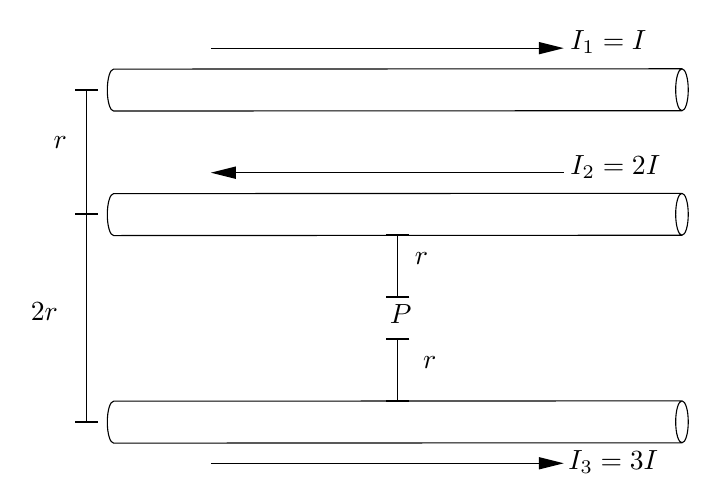
\begin{tikzpicture}[x=0.75pt,y=0.75pt,yscale=-1,xscale=1]
    \draw   (436.97,250.14) -- (163.14,250.29) .. controls (161.46,250.29) and (160.1,245.77) .. (160.1,240.19) .. controls (160.1,234.61) and (161.46,230.09) .. (163.13,230.09) -- (436.96,229.94) .. controls (438.64,229.94) and (439.99,234.46) .. (440,240.04) .. controls (440,245.62) and (438.64,250.14) .. (436.97,250.14) .. controls (435.3,250.14) and (433.94,245.62) .. (433.94,240.04) .. controls (433.93,234.47) and (435.29,229.94) .. (436.96,229.94) ;
    \draw   (436.97,150.14) -- (163.14,150.29) .. controls (161.46,150.29) and (160.1,145.77) .. (160.1,140.19) .. controls (160.1,134.61) and (161.46,130.09) .. (163.13,130.09) -- (436.96,129.94) .. controls (438.64,129.94) and (439.99,134.46) .. (440,140.04) .. controls (440,145.62) and (438.64,150.14) .. (436.97,150.14) .. controls (435.3,150.14) and (433.94,145.62) .. (433.94,140.04) .. controls (433.93,134.47) and (435.29,129.94) .. (436.96,129.94) ;
    \draw   (436.97,90.14) -- (163.14,90.29) .. controls (161.46,90.29) and (160.1,85.77) .. (160.1,80.19) .. controls (160.1,74.61) and (161.46,70.09) .. (163.13,70.09) -- (436.96,69.94) .. controls (438.64,69.94) and (439.99,74.46) .. (440,80.04) .. controls (440,85.62) and (438.64,90.14) .. (436.97,90.14) .. controls (435.3,90.14) and (433.94,85.62) .. (433.94,80.04) .. controls (433.93,74.47) and (435.29,69.94) .. (436.96,69.94) ;
    \draw    (150,80) -- (150,140) ;
    \draw [shift={(150,140)}, rotate = 270] [color={rgb, 255:red, 0; green, 0; blue, 0 }  ][line width=0.75]    (0,5.59) -- (0,-5.59)   ;
    \draw [shift={(150,80)}, rotate = 270] [color={rgb, 255:red, 0; green, 0; blue, 0 }  ][line width=0.75]    (0,5.59) -- (0,-5.59)   ;
    \draw    (150,140) -- (150,240) ;
    \draw [shift={(150,240)}, rotate = 270] [color={rgb, 255:red, 0; green, 0; blue, 0 }  ][line width=0.75]    (0,5.59) -- (0,-5.59)   ;
    \draw [shift={(150,140)}, rotate = 270] [color={rgb, 255:red, 0; green, 0; blue, 0 }  ][line width=0.75]    (0,5.59) -- (0,-5.59)   ;
    \draw    (210,60) -- (378,60) ;
    \draw [shift={(380,60)}, rotate = 180] [fill={rgb, 255:red, 0; green, 0; blue, 0 }  ][line width=0.08]  [draw opacity=0] (12,-3) -- (0,0) -- (12,3) -- cycle    ;
    \draw    (380,120) -- (212,120) ;
    \draw [shift={(210,120)}, rotate = 360] [fill={rgb, 255:red, 0; green, 0; blue, 0 }  ][line width=0.08]  [draw opacity=0] (12,-3) -- (0,0) -- (12,3) -- cycle    ;
    \draw    (210,260) -- (378,260) ;
    \draw [shift={(380,260)}, rotate = 180] [fill={rgb, 255:red, 0; green, 0; blue, 0 }  ][line width=0.08]  [draw opacity=0] (12,-3) -- (0,0) -- (12,3) -- cycle    ;
    \draw    (300,150) -- (300,180) ;
    \draw [shift={(300,180)}, rotate = 270] [color={rgb, 255:red, 0; green, 0; blue, 0 }  ][line width=0.75]    (0,5.59) -- (0,-5.59)   ;
    \draw [shift={(300,150)}, rotate = 270] [color={rgb, 255:red, 0; green, 0; blue, 0 }  ][line width=0.75]    (0,5.59) -- (0,-5.59)   ;
    \draw    (300,200) -- (300,230) ;
    \draw [shift={(300,230)}, rotate = 270] [color={rgb, 255:red, 0; green, 0; blue, 0 }  ][line width=0.75]    (0,5.59) -- (0,-5.59)   ;
    \draw [shift={(300,200)}, rotate = 270] [color={rgb, 255:red, 0; green, 0; blue, 0 }  ][line width=0.75]    (0,5.59) -- (0,-5.59)   ;
    \draw (133,101.4) node [anchor=north west][inner sep=0.75pt]    {$r$};
    \draw (122,181.4) node [anchor=north west][inner sep=0.75pt]    {$2r$};
    \draw (307,157.4) node [anchor=north west][inner sep=0.75pt]    {$r$};
    \draw (311,207.4) node [anchor=north west][inner sep=0.75pt]    {$r$};
    \draw (295,182.4) node [anchor=north west][inner sep=0.75pt]    {$P$};
    \draw (382,50.4) node [anchor=north west][inner sep=0.75pt]    {$I_{1} =I$};
    \draw (382,110.4) node [anchor=north west][inner sep=0.75pt]    {$I_{2} =2I$};
    \draw (381,252.4) node [anchor=north west][inner sep=0.75pt]    {$I_{3} =3I$};
    \end{tikzpicture}
    \caption{3 Coplanar Wires}
\end{figure}

From the right hand rule, we find that $I_1$ and $I_3$ will have magnetic fields coming out of the page at the top, and in at the bottom, while $I_2$ will be out at the bottom and in at the top, as in Figure~\ref{sideviewthreewires}.
\begin{figure}[h!t]\label{sideviewthreewires}
    \centering
    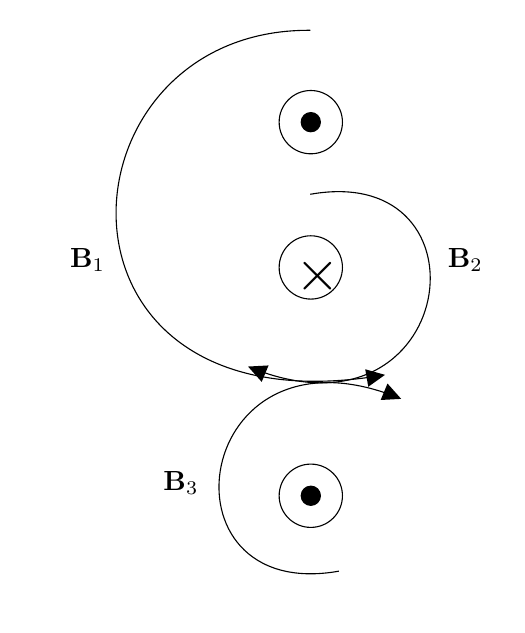
\begin{tikzpicture}[x=0.75pt,y=0.75pt,yscale=-1,xscale=1]
    %uncomment if require: \path (0,300); %set diagram left start at 0, and has height of 300
    
    %Shape: Circle [id:dp952640352341813] 
    \draw   (330,55.25) .. controls (330,46.83) and (336.83,40) .. (345.25,40) .. controls (353.67,40) and (360.5,46.83) .. (360.5,55.25) .. controls (360.5,63.67) and (353.67,70.5) .. (345.25,70.5) .. controls (336.83,70.5) and (330,63.67) .. (330,55.25) -- cycle ;
    %Shape: Circle [id:dp640071140525873] 
    \draw   (330,125.25) .. controls (330,116.83) and (336.83,110) .. (345.25,110) .. controls (353.67,110) and (360.5,116.83) .. (360.5,125.25) .. controls (360.5,133.67) and (353.67,140.5) .. (345.25,140.5) .. controls (336.83,140.5) and (330,133.67) .. (330,125.25) -- cycle ;
    %Shape: Circle [id:dp29098052519862794] 
    \draw   (330,235.25) .. controls (330,226.83) and (336.83,220) .. (345.25,220) .. controls (353.67,220) and (360.5,226.83) .. (360.5,235.25) .. controls (360.5,243.67) and (353.67,250.5) .. (345.25,250.5) .. controls (336.83,250.5) and (330,243.67) .. (330,235.25) -- cycle ;
    %Shape: Circle [id:dp09033906722413998] 
    \draw  [fill={rgb, 255:red, 0; green, 0; blue, 0 }  ,fill opacity=1 ] (340.63,55.25) .. controls (340.63,52.7) and (342.7,50.63) .. (345.25,50.63) .. controls (347.8,50.63) and (349.88,52.7) .. (349.88,55.25) .. controls (349.88,57.8) and (347.8,59.88) .. (345.25,59.88) .. controls (342.7,59.88) and (340.63,57.8) .. (340.63,55.25) -- cycle ;
    %Shape: Circle [id:dp7746686710566881] 
    \draw  [fill={rgb, 255:red, 0; green, 0; blue, 0 }  ,fill opacity=1 ] (340.63,235.25) .. controls (340.63,232.7) and (342.7,230.63) .. (345.25,230.63) .. controls (347.8,230.63) and (349.88,232.7) .. (349.88,235.25) .. controls (349.88,237.8) and (347.8,239.88) .. (345.25,239.88) .. controls (342.7,239.88) and (340.63,237.8) .. (340.63,235.25) -- cycle ;
    %Curve Lines [id:da14168924830348262] 
    \draw    (345,11) .. controls (220.62,10) and (209.11,205.03) .. (378.43,177.43) ;
    \draw [shift={(381,177)}, rotate = 530.11] [fill={rgb, 255:red, 0; green, 0; blue, 0 }  ][line width=0.08]  [draw opacity=0] (8.93,-4.29) -- (0,0) -- (8.93,4.29) -- cycle    ;
    %Curve Lines [id:da6939861555194753] 
    \draw    (345,90) .. controls (434.55,74.08) and (416.19,213.59) .. (316.51,173.62) ;
    \draw [shift={(315,173)}, rotate = 382.58000000000004] [fill={rgb, 255:red, 0; green, 0; blue, 0 }  ][line width=0.08]  [draw opacity=0] (8.93,-4.29) -- (0,0) -- (8.93,4.29) -- cycle    ;
    %Shape: Boxed Bezier Curve [id:dp12013228880681281] 
    \draw    (358.8,271.58) .. controls (269.25,287.5) and (287.61,147.98) .. (387.29,187.96) ;
    \draw [shift={(388.8,188.58)}, rotate = 202.57999999999998] [fill={rgb, 255:red, 0; green, 0; blue, 0 }  ][line width=0.08]  [draw opacity=0] (8.93,-4.29) -- (0,0) -- (8.93,4.29) -- cycle    ;
    
    % Text Node
    \draw (336.5,119) node [anchor=north west][inner sep=0.75pt]    {\huge$\times $};
    % Text Node
    \draw (228, 115) node [anchor=north west][inner sep=0.75pt]    {$\mathbf{B}_{1}$};
    % Text Node
    \draw (410, 115) node [anchor=north west][inner sep=0.75pt]    {$\mathbf{B}_{2}$};
    % Text Node
    \draw (273,222.4) node [anchor=north west][inner sep=0.75pt]    {$\mathbf{B}_{3}$};
    \end{tikzpicture}
    \caption{Side View with Magnetic Field}
\end{figure}
Thus, this equates to three vectors at point $P$: $\mathbf{B}_1$ to the right, and $\mathbf{B}_2$ and $\mathbf{B}_3$ to the left. Then, we have
\begin{align*}
    \mathbf{B}_1 &= \frac{\mu_0 I}{4\pi r}, \\
    \mathbf{B}_2 &= \frac{\mu_0 I}{\pi r}, \\
    \mathbf{B}_4 &= \frac{3\mu_0 I}{2\pi r}.
\end{align*}
Adding these together yields
\[\mathbf{B} = \frac{\mu_0 I}{\pi r} + \frac{3\mu_0 I}{2\pi r} - \frac{\mu_0 I}{4\pi r},\]
such that \[\mathbf{B} = \boxed{\frac{9\mu_0 I}{4\pi r}}.\]

\section{Biot-Savart Law}
The Biot-Savart law was originally discovered by Jean-Baptiste Biot and F\'elix Savart, and relates current, distance, and shape to the magnetic field. Conceptually, we can split a non-linear current carrying wire into infinitesimal linear pieces and find their contributions to magnetic field.
\begin{thrm}[Biot-Savart Law]
    For a piece of wire with length $\dd \ell$ at a distance $r$,
    \begin{equation}
        \dd \mathbf{B} = \frac{\mu_0}{4\pi} \frac{I\dd \vec{\ell} \times \vu{r}}{r^2}.
    \end{equation}
\end{thrm}
Recall that $\vu{r}$ is the unit vector pointing radially outwards, in the direction of $r$. Additionally, $\dd \vec{\ell} \times \vu{r}$ can also be expressed as $\dd \ell \sin\theta$.

Suppose that we have a wire of length $\ell$ carrying current $I$. At a point $P$ which is $r$ meters away from each section of wire,
\begin{align*}
    \dd \mathbf{B} &= \frac{\mu_0 I}{4\pi} \frac{\dd \ell \sin\theta}{r^2} \\
    \mathbf{B} &= \frac{\mu_0 I}{4\pi} \int \frac{\dd \ell \sin\theta}{r^2}.
\end{align*}
\subsection{Magnetic Field of a Coil}
Suppose we have a coil of wire with radius $r$ and current $I$. Then, as $\dd \ell$ is tangent to the coil, we have that $\dd \vec{\ell} \perp \vu{r}$, so $\dd \vec{\ell} = \dd \ell$. Then, we have
\[\dd \mathbf{B} = \frac{\mu_0I}{4\pi} \frac{\dd l}{r^2}.\]
Integrating on both sides gives
\[\mathbf{B} = \frac{\mu_0I}{4\pi r^2} \cdot 2\pi r,\]
so $\mathbf{B} = \frac{\mu_0I}{2r}$. With $N$ loops, we multiply this quantity by $N$.
\subsection{Magnetic Field of an Infinite Wire}
Suppose we have a long wire of infinite length, and we select a point $P$ next to it. For each small $\dd \vec{\ell}$, there will be a small contribution of $\dd \mathbf{B}$. If point $P$ is a distance $r$ away from $\dd \vec{\ell},$ we can describe $r$ as $\frac{R}{\sin\theta},$ where $\theta$ is the angle between the wire and $r$. We can also express $\ell$ as $R\cot\theta$, meaning that $\dd \ell = -R\csc^2\theta\dd\theta$. Then, we have
\[\mathbf{B} = \int_{-\infty}^{\infty} \dd \mathbf{B} = 2\int_0^{\infty} \dd \mathbf{B}.\]
From the Biot-Savart law,
\begin{align*}
    \mathbf{B} &= \frac{\mu_0 I}{2\pi} \int_{0}^{\infty} \frac{\dd\ell\sin\theta}{r^2} \\
    &= \frac{\mu_0 I}{2\pi} \int_{\pi/2}^{0} \frac{-R\dd\theta}{\sin^2\theta} \sin\theta \p{\frac{\sin^2\theta}{R^2}} \\
    &= -\frac{\mu_0 I}{2\pi R}\int_{\pi/2}^{0} \sin\theta\dd \theta \\
    &= \frac{\mu_0I}{2\pi R}\p{\cos \theta\Big|_{\pi/2}^0} \\
    &= \frac{\mu_0 I}{2\pi R}.
\end{align*}
This result is identical to that derived via Amp\` ere's law.

\section{Force Between Two Parallel Wires}
Suppose we have two wires with currents $I_1$ and $I_2$, separated by distance $r$ and pointing to the right such that $I_1$ is higher than $I_2$. Then, $I_1$ creates a magnetic field into the plane of the page at $I_2$. Similarly, $I_2$ creates a field \textit{out} of the plane of the page at $I_1$.

Focusing on $I_2$, note that
\begin{equation}
    B_1 = \frac{\mu_0 I}{2\pi r}.
\end{equation}
Furthermore, $F_2 = ILB$, meaning that
\begin{equation}
    F_2 = F_1 = \frac{\mu_0 \ell I_1I_2}{2\pi r}.
\end{equation}
From the right hand rule, force will be pointed to the other wire. Thus, the wires will \textbf{attract}.

Now suppose that we have that $I_2$ is opposing $I_1$ in direction. Then, $\mathbf{B}_2$ and $\mathbf{B}_1$ are pointed into the plane of the page. Thus, from the right hand rule, force will be outwards from both, meaning that the wires will \textbf{repel}.

\section{Ampere's Law}
Ampere's Law is stated as
\begin{thrm}[Ampere's Law]
    The magnetic field on an Amperian loop with current $I$ is
    \begin{equation}
        \oint \mathbf{B} \cdot \dd \vec{\ell} = \mu_0 I_{\mathrm{enc}}.
    \end{equation}
\end{thrm}
Much like Gauss's law, we take the field dotted with a small piece of the loop, and equate that to a constant multiplied by the current. To use this, we often use \textit{charge density} to find the amount of charge along some length $\dd \ell$. The $\oint$ symbol refers to a \textbf{closed line integral}.

Suppose we have a long current-carrying wire with current $I$ and radius $R$. To determine the magnetic field around the wire, we create Amperian loops \textbf{concentric} with the wire (similar to Gaussian surfaces). Then, we have
\[\oint \mathbf{B} \cdot \dd \ell = \mu_0 I.\]
For a point at a distance $r$ away from the wire, the Amperian loop has length $2\pi r$, giving us
\[\mathbf{B}(2\pi r) = \mu_0 I,\]
so
\begin{equation}
    \mathbf{B} = \frac{\mu_0 I}{2\pi r}.
\end{equation}
Inside the wire, we have that the current density is given by
\[J = \frac{I}{A} = \frac{I}{\pi R^2}.\]
Again, we have
\[\mathbf{B} \cdot 2\pi r = \mu_0 I_{\mathrm{enc}}.\]
To find $I_{\mathrm{enc}},$ we have
\begin{align*}
    I_{\mathrm{enc}} &= JA_{\mathrm{enc}}
    &= \frac{I \pi r^2}{\pi R^2}.
\end{align*}
Thus, we have
\begin{equation}
    \mathbf{B} = \frac{\mu_0 I r}{2\pi R^2}.
\end{equation}

\subsection{Magnetic Field of a Solenoid}
A solenoid is defined as a tightly compacted coil of wire, with $N$ turns, a length $\ell$, and a radius $r$. An ``ideal'' solenoid is infinitely long with very tightly coiled loops. When it carries current $I$, a regular magnetic field is created. The magnetic field is 0 outside of the solenoid, and the field direction is found using the right-hand-rule for wires.

To determine the Amperian component, we consider a rectangular loop horizontally around the wires in the loop. Rather than integrating to determine the magnetic field of this loop, we take the sum $\Sigma \mathbf{B} \dd \ell$. However, the vertical components of this loop and the upper component (outside the solenoid) are zero, giving us that $\Sigma \mathbf{B} \dd \ell$ is $\mathbf{B}_{\mathrm{b}}\ell = \mu_0 I_{\mathrm{enc}}$, where $\mathbf{B}_b$ is the magnetic field of the bottom part of the loop (center of the solenoid).

To find $I_{\mathrm{enc}}$, we have that $I_{\mathrm{enc}} = IN$. Additionally, $\frac{N}{\ell}$ is a constant defined as $n$, the number of loops per length. Then, we have
\begin{equation}
    \mathbf{B} = \mu_0 n I.
\end{equation}

\subsection{Magnetic Field of a Coaxial Cable}
A coaxial cable is made of an inner and outer conductor, separated by an insulating medium, such that the inner and outer components have currents in opposite directions.
\begin{example}[1994 E3]
    A long coaxial cable consists of a solid cylindrical conductor of radius $a$, surrounded by a hollow coaxial conductor of inner radius $b$ and outer radius $c$. The two conductors each carry a uniformly distributed current $I$, but in opposite directions. The current is to the right in the outer cylinder and to the left in the inner cylinder. Assume $\mu = \mu_0$ for all materials in this problem.
    \begin{enumerate}[label=\alph*.]
        \item Use Ampere's law to determine the magnitude of the magnetic field at a distance $r$ from the axis of the cable in each of the following cases:
        \begin{enumerate}[label=\roman*.]
            \item $0 < r < a$
            \item $a < r < b$
        \end{enumerate}
        \item What is the magnitude of the magnetic field at a distance $r = 2c$ from the axis of the cable?
    \end{enumerate}
\end{example}
\begin{solution}
    For part i, consider an Amperian loop concurrently within the larger conductor. Then, the current density is given as
    \[J = \frac{I}{\pi a^2},\]
    so that
    \[I_{\mathrm{enc}} = \frac{Ir^2}{a^2}.\]
    Thus, we have
    \[\mathbf{B} = \frac{\mu_0 I r}{2\pi a^2}.\]
    For part ii, consider an Amperian loop concurrently around the inner wire. Then, we have
    \[\mathbf{B} \cdot 2\pi r = \mu_0 I,\]
    as $I_{\mathrm{enc}} = I$. Thus, $\mathbf{B} = \frac{\mu_0 I}{2\pi r}.$ For part (b), note again that
    \[\mathbf{B} \cdot 2\pi r = \mu_o (I - I),\]
    so $\mathbf{B} = 0$.
\end{solution}

\subsection{Magnetic Field at the Center of a Solenoid}
Consider a cross section of a solenoid such that on the left hand side, current flows into the page, and on the right, it flows out. Then, the magnetic field of each wire create a magnetic field of zero on the edge of the solenoid, and a strong field in the center.

We create an Amperian loop to infinity which surrounds two wires with current into the page. Then, $I_{\mathrm{enc}} = 2I$, so we have
\begin{align*}
    \mu_0 I_{\mathrm{enc}} &= \oint \mathbf{B} \cdot \dd \vec{\ell} \\
    2I\mu_0 &= \int_{a}^b \mathbf{B} \cdot \dd \vec{\ell} + \int_{b}^c \mathbf{B} \cdot \dd \vec{\ell} + \int_{c}^d \mathbf{B} \cdot \dd \vec{\ell} + \int_{d}^a \mathbf{B} \cdot \dd \vec{\ell},
\end{align*}
where $a,b,c$ and $d$ are points on the loop such that $a$ and $b$ are inside the solenoid and $c$ and $d$ are outside. However, the integral from $c$ to $b$ (and vice versa) will become zero as $\mathbf{B} \perp \dd \vec{\ell}$. Additionally, $\mathbf{B} = 0$ from $c$ to $d$. Thus, we have
\[2\mu_0 I = \int_a^b B\,\dd \ell,\]
as $\mathbf{B} \perp \dd \vec{\ell}$. This integral becomes
\[2\mu_0I = B(h),\]
where $h$ is the distance from $a$ to $b$. Thus,
\[B = \frac{2\mu_0 I}{h}.\]
However, in a solenoid, there are $N$ loops rather than simply 2, giving us
\begin{equation}
    \mathbf{B} = \frac{\mu_0 NI}{h},
\end{equation}
or equivalently
\[\mathbf{B} = \mu_0 n I,\]
where $n$ is the turn density.

\subsection{Magnetic Field due to a Toroid}
A toroid is a solenoid in the shape of a torus, as in the figure. Suppose, as with the solenoid, that we cut the toroid in half such that the outer circle has inward current and the inner circle has outward current. From the right-hand rule, field will point counterclockwise within the torus. Ampere's law yields
\[\mu_0 I_{\mathrm{enc}} = \oint \mathbf{B} \cdot \dd\vec{\ell}.\]
If there are $N$ coils, $I_{\mathrm{enc}} = NI$, so we have
\[\mu_0 NI = B(2\pi r),\]
giving us
\begin{equation}
    \mathbf{B} = \frac{\mu_0 NI}{2\pi r}.
\end{equation}
In the inner circle, or outside the torus, the field is 0.

\begin{figure}[t!]
    \centering
    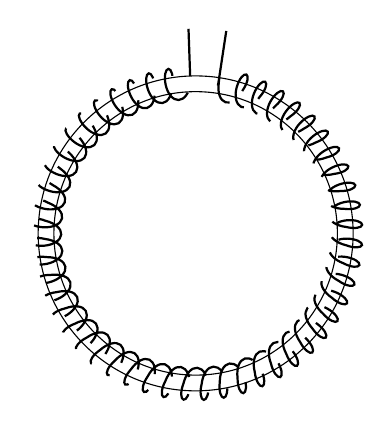
\begin{tikzpicture}[decoration={coil, amplitude=2mm, segment length=2.3mm}
                    ]
    \draw (0,0)   circle[radius=2];
    \draw (0,0)   circle[radius=1.8];
    \draw [thick,black](92:2) -- (92:2.6);
    \draw [thick,black](441.4:1.9) -- (441.4:2.6);
    \draw[decorate,thick,black, dash pattern = on 21.5pt off 6.3pt, dash phase=24.5pt] 
        (92:1.9) arc[start angle=92, end angle=441.5, radius=1.9];
    \end{tikzpicture}
    \caption{A toroid}
\end{figure}

\subsection{Magnetic Field due to a Current Carrying Sheet}
Suppose we have a current carrying sheet of width $d$ with current density $J$. From the right hand rule, if $I$ points inwards, the magnetic field will be to the right above the sheet and to the left below it.

Take an Amperian loop in the shape of a rectangle with length $x$ and width $y$. Then, we have
\begin{align*}
    \oint \mathbf{B} \cdot \dd \vec{\ell} &= \mu_0 J(yd) \\
    2B\int_{A}^B \dd \vec{\ell} &= \mu_0 Jyd,
\end{align*}
where $A$ and $B$ are the points at the top of the loop. The vertical segments of the loop contribute no magnetic field. Thus,
\[2By = \mu_0 Jyd,\]
so
\begin{equation}
    \mathbf{B} = \frac{\mu_0 Jd}{2}.
\end{equation}

\section{Magnetic Flux and Faraday's Law}
Magnetic flux is similar to electric flux, in that it measures the amount of magnetic field passing through an area. It is given by
\begin{equation}
    \Phi_B = \int \mathbf{B} \cdot \dd \vec{A}.
\end{equation}
This simplifies to $\Phi_B = BA\cos\theta$ for well-defined areas.
\begin{example}[2012 E3]
    A closed loop is made of a U-shaped metal wire of negligible resistance and a movable metal crossbar of resistance $R$. The crossbar has mass $m$ and length $L$. It is initially located a distance $h_0$ from the other end of the loop. The loop is placed vertically in a uniform horizontal magnetic field of magnitude $B_0$ into the plane of the paper. Determine the magnitude of the magnetic flux through the loop.
\end{example}
\begin{solution}
    Since $\theta = 0$, we have $\cost = 1$, so $\Phi_B = B_0Lh_0$.    
\end{solution}
\begin{example}[2013 E3]\label{2013E3}
    A circular wire loop with radius 0.10 m and resistance 50 $\Omega$ is held in place horizontally in a magnetic field $\mathbf{B}$ directed upwards at an angle of 60$\degr$ with the vertical. The magnetic field is given as a function of time $t$ by $B(t) = 4(1-0.2t)$. Derive an expression for the magnetic flux through the loop as a function of time $t$.
\end{example}
\begin{solution}
    As $B = 4 - 0.8t$, we then have $I = (5-0.8t)(\pi r^2)\cos(60).$ This simplifies to $0.67 - 0.13t$.
\end{solution}

\subsection{Faraday's Law}
In 1831, Faraday found that a changing magnetic field through a coil of wire creates a current in that wire, called the ``induced current.'' This induced current is actually caused by an induced emf $\mathcal{E}$, which is generated by changing the field, loop area, or loop orientation.
\begin{thrm}
    The induced emf caused by a change in flux is
    \begin{equation}
        \mathcal{E} = - \dv{\Phi_B}{t}.
    \end{equation}
\end{thrm}
Suppose we have is a metal bar on rails, such that the bar lies vertically and perpendicular to magnetic field coming out of the page, and the rails have height $h$ parallel to the bar and length $\ell$ perpendicular to it. Then, we have
\[\mathcal{E} = -\dv{\Phi_B}{t}.\]
Over time, the only change in flux is $\ell$, giving us
\[\mathcal{E} = -Bh\dv{l}{t} = -Bhv.\]

\begin{example}[2013 E3]
    Suppose that we have the same setup as Example~\ref{2013E3}. Calculate a numerical value of the induced emf in the loop.
\end{example}
\begin{solution}
    As $\mathcal{E}$ is the derivative of flux, we simply have
    \[\mathcal{E} = -\dv{\Phi_B}{t} = \dv{t} (0.063 - 0.013t),\]
    or $\boxed{0.013 V}$.
\end{solution}
\begin{example}
    A circular loop of area 0.25 $m^2$ and resistance 12 $\Omega$ lies in the plane of the page. The magnetic field is given by $B = 1.8e^{-0.05t}$ from times $t = 0$ to $t = 8$.
    \begin{enumerate}[label=\roman*.]
        \item Derive an expression for the magnitude of the induced emf in the loop as a function of time for the interval $t = 0$ to $t = 8$ s.
        \item Calculate the magnitude of the induced current $I$ in the loop at time $t= 4$ s.
    \end{enumerate}
\end{example}
\begin{solution}
    For part (i), we take the derivative, giving us
    \begin{align*}
        \mathcal{E} &= - \dv{\Phi_B}{t} \\
        &= A\dv{B}{t} \\
        &= (0.25)(1.8)(0.05)(1.8)e^{-0.05t} \\
        &= \boxed{0.0225e^{-0.5t}}.
    \end{align*}
    For part (ii), we have
    \[I = \frac{\mathcal{E}}{R},\]
    giving us $\boxed{1.54 mA}$.
\end{solution}

\section{Lenz's Law}
Recall that Faraday's Law is used to calculate the magnitude of an induced emf and current. Lenz's Law is used to find the \textbf{direction} of the induced current. Lenz's Law is a statement of conservation of energy.
\begin{thrm}[Lenz's Law]
    The induced current of a magnetic object will create its own magnetic field, opposing the change in magnetic flux.
\end{thrm}
To apply Lenz's Law, use the following procedure:
\begin{enumerate}[noitemsep]
    \item Determine the direction of the magnetic field in the loop.
    \item Determine whether the flux is decreasing or increasing.
    \item If the flux is \textbf{increasing}, the induced current must create a magnetic field \textbf{opposite} to the direction of the current magnetic field.
    \item If the flux is \textbf{decreasing}, the induced current must create a magnetic field \textbf{parallel} to the direction of the current magnetic field.
\end{enumerate}
\begin{example}
    A bar lies on a U-shaped metal rod with velocity pointed to the right. Passing through the loop is a magnetic field going out of the page. What is the direction of the induced current.
\end{example}
\begin{solution}
    Recalling that $\Phi_B \propto A$, we have that $\dv{A}{t} > 0$ means that $dv{\Phi_B}{t}$. Thus, since flux increases, the magnetic field is opposite, or into the page. Then, the induced current is clockwise.    
\end{solution}

\subsection{Force vs. Torque on a Conductive Loop}
As a result of change in flux, wires and loops can experience net torque and net force. If the forces are unbalanced, the wire/loops will have linear acceleration, and if the torques are unbalanced, the wires/loops will have rotational acceleration.

Suppose we have a wire loop in a magnetic field, such that $\mathbf{B}$ points to the right (parallel to the plane of the loop), and current points counterclockwise around the loop. For the bottom and top pieces of the wire, force will be zero, trivially.

For the left and right pieces, the forces will be nonzero. However, they will cancel each other out, such that $\Sigma F = 0$, but $\Sigma \tau \ne 0$.

Now suppose we have a similar situation, but with a $45\degr$ angle between the magnetic field and area vector. Still, $\Sigma F = 0$, but $\Sigma \tau \neq 0$ (but it will be smaller than before).

Finally, suppose we have an angle of 0 degrees (i.e. $\vec{A} \perp \mathbf{B}$). Then, $\Sigma F = \Sigma \tau = 0$.

\section{Applications of Faraday's Law}
Suppose we have a loop of wire of width $w$ and height $h$, with a switch and battery, which is connected to a spring with force constant $k$ (recall that $F_s = -kx$). Let the loop carry current $I$ in a clockwise direction, and the bottom half be in a uniform magnetic field direction into the page.

Say that the switch is opened, and the loop comes to rest at a new equilibrium position a distance $x$ from the original position. Observe that force will be pointed down on the bottom piece, to the left on the left piece, and to the right on the right piece. Then we have that
\begin{align*}
    F_B &= F_S \\
    IwB &= kx \\
    B &= \frac{kx}{Iw}.
\end{align*}
Then, say that the spring is replaced with a loop of the same dimensions, but with resistance $R$ and no battery or switch. The loop is pulled upwards, with constant speed $v_0$. This means that by the RHR, as flux decreases with the decreasing magnetic field, magnetic field must also go into the page and current is counterclockwise. We also then have
\[\mathcal{E} = B \dv{A}{t},\]
or $Bw\dv{h}{t} = Bwv_0$. Then, $I = \frac{Bwv_0}{R}$.

Finally, the power dissipated in the loop is just $P = I^2R = \frac{B^2w^2v^2_0}{R}$.

\section{Differential Equation Applications of Faraday's Law}
Suppose that a conducting bar with mass $M$ and length $L$ is connected to two long vertical rails, which are connected by a resistor of resistance $R$ at the top. This system is located in a field $B$ going into the page. The bar is released from rest and slides down the rails without friction.

In this case, the flux goes up as the bar slides down, so the magnetic field must go out of the page, so the current in the resistor is to the left. Further, we can find the velocity of the bar as a function of time $t$ using differential equations. We have that
\[\Sigma F = mg - ILB,\]
where $I = \frac{E}{R},$ which is then $\frac{BLv}{R}$. Subsituting this gives us
\begin{align*}
    Ma &= Mg - \frac{B^2L^2v}{R} \\
    \dv{v}{t} &= g - \frac{B^2L^2v}{MR}.    
\end{align*}
The terminal velocity will occur when $a = 0$, so $v_T = \frac{MgR}{B^2L^2}$. This is very similar to drag force. To determine the power dissipated in the resistor, we use $P = I^2R,$ giving us $P = \frac{B^2L^2v_T^2}{R}$.

To solve the differential equation, we can use separation of variables by factoring out the $B^2L^2/MR$ term, so we have
\begin{align*}
    \dv{v}{t} = \frac{B^2L^2}{MR}\p{\frac{MRg}{B^2L^2} - v} \\
    \frac{\dd v}{\frac{MRg}{B^2L^2} - v} &= \frac{B^2L^2}{MR} \dd t \\
    \int_0^v \frac{\dd v}{\frac{MRg}{B^2L^2} - v} &= \frac{B^2L^2}{MR} \int_0^t \dd t \\
    - \ln\p{\frac{MRg}{B^2L^2} - v} + \ln\p{\frac{MRg}{B^2L^2}} &= \frac{B^2L^2}{MR} t \\
    \frac{\frac{MRg}{B^2L^2}}{\frac{MRg}{B^2L^2}-v} &= e^\frac{B^2L^2t}{MR} \\
    \frac{MRg}{B^2L^2}- \frac{\frac{MRg}{B^2L^2}}{e^\frac{B^2L^2t}{MR}} &= v \\
    v&= \frac{MRg}{B^2L^2}\p{1-e^{-\frac{B^2L^2t}{MR}}}.
\end{align*}

\section{Inductors and Inductance}
In a circuit, an inductor is a coil of wire which self-induces an emf and current. An inductor has an \textbf{inductance} $L$, given by
\begin{equation}
    L = N \cdot \frac{\Phi_B}{I},
\end{equation}
which is measured in Henrys (H). Inductors in circuits will always oppose changes in the current in that circuit. For this reason, they are often used in surge protectors, as they will oppose any rapid change in current during a power surge.

We can analyze their behavior using equations derived from Faraday's Law of Inductors, which states
\begin{equation}
    \oint \mathbf{E} \cdot \dd\vec{\ell} = -\dv{\Phi_B}{t}.
\end{equation}
We also know that the integral resolves to $Ed = \mathcal{E}$, and we know that
\[L\dv{I}{t} = \dv{\Phi_B}{t},\]
so we thus have
\begin{equation}
    \mathcal{E} = -L\dv{I}{t}.
\end{equation}

For a solenoid, consider the flux equation $\Phi_B = BA$. We know that the field is
\[B = \mu_0 n I = \frac{\mu_0 NI}{\ell}.\]
Then, we find
\[\Phi_B = \frac{A\mu_0 NI}{\ell}.\]
Substituting this in the inductance equation, we have
\begin{equation}
    L = \frac{\mu_0 N^2A}{\ell}.
\end{equation}

For a more conceptual understanding of inductance, we can write $L$ as
\[-\frac{\mathcal{E}}{\dv{I}{t}}.\]
This means that a larger $L$ corresponds with a greater decrease in change in current.
\section{LR Circuits}
Inductors can act similarly to batteries or resistors, moving or slowing the current. It's important to look at the steady-state behavior of inductors, as with capacitors. Consider the LR circuit below.
\begin{figure}[h!]
    \centering
    \begin{circuitikz}[]
        \draw (0, 0) to[R] (3, 0) to[cute inductor] (3, 3) -- (0, 3) to[battery] (0, 0);
    \end{circuitikz}
    \caption{LR Circuit}
\end{figure}
As current flows, there will be an increase in voltage across the battery, and a decrease in voltage of $IR$ across the resistor. With the inductor, if $I$ is constant, there will be constant voltage (i.e. like a wire). If $\dv{I}{t} > 0$, there will be a \textbf{decrease} in voltage (i.e. like a resistor), and if $\dv{I}{t} < 0$, there will be an \textbf{increase} (like a battery).

Suppose that the circuit contains a switch, and let the inductor have inductance $L = 15 mH$, the battery have voltage $20 V$, and the resistor have resistance $10\Omega$. Then, immediately after the switch is closed, the current will be zero, as the inductor pushes back against the increase in current. After some time, we can say that the inductor will act like a wire, so we have $I = V/R = 2$ A.

We know derive exponential equations for the behavior of LR circuits. With Kirchhoff's rules, observe that
\[\mathcal{E} - L\dv{I}{t} - IR = 0.\]
Rearranging and separating variables, we find
\begin{align*}
    \frac{\dd t}{L} &= \frac{\dd I}{\mathcal{E} - IR} \\
    \int_0^t \frac{1}{L} \dd t &= \int_0^I \frac{1}{\mathcal{E} - IR} \dd I \\
    \frac{t}{L} &= -\frac{1}{R} \cdot \ln\p{\frac{\mathcal{E} - IR}{\mathcal{E}}} \\
    e^{-Rt/L} &= \frac{\mathcal{E} - IR}{\mathcal{E}} \\
    IR &= \mathcal{E} - \mathcal{E}e^{-Rt/L}.
\end{align*}
Dividing by $R$ and substituting $I_f = \frac{\mathcal{E}}{R}$ gives
\begin{equation}
    I(t) = I_f\p{1-e^{-\frac{Rt}{L}}}.
\end{equation}
We define the time constant $\tau$ as $L/R$.
\begin{example}[2005 E2]
    In the circuit below, resistors 1 and 2 of resistance $R_1$ and $R_2$, respectively, and an inductor of inductance $L$ are connected to a battery of emf $\mathcal{E}$ and a switch $S$. The switch is closed at time $t = 0$. Express all algebraic answers in terms of the given quantities and fundamental constants.
    \begin{enumerate}[label=(\alph*), noitemsep, topsep=5pt]
        \item Determine the current through resistor 1 immediately after the switch is closed.
        \item Determine the magnitude of the initial rate of change of current $\dd I/\dd t$, in the inductor.
        \item Determine the current through the battery a long time after the switch has been closed.
        \item Sketch a graph of the current through the battery as a function of time.
        \item Determine the voltage across resistor 2 just after the switch is opened, some time after steady state has been reached.
    \end{enumerate}
    \begin{center}
        \centering
        \begin{tikzpicture}
            \draw (0, 0) -- (6, 0) to[cute inductor=$L$] (6, 2) -- (3.5, 2) to[R=$R_1$] (2, 2) to[nos=$S$] (0, 2) to[battery1=$\mathcal{E}$] (0, 0);
            \draw (4.5, 0) to[R=$R_2$] (4.5, 2);
        \end{tikzpicture}
    \end{center}
\end{example}
\begin{solution}
    After the switch is closed, current begins to flow through the circuit. As there was initially no current, $\Delta I/\Delta t$ is positive, meaning that $L$ will act like a resistor or a reverse battery. Thus, there will be no current in the branch with the inductor.
    
    The above setup then implies that the circuit is effectively just two resistors in parallel, meaning that we can say \[I = \boxed{\frac{\mathcal{E}}{R_1+R_2}}.\]
    
    Then, note that since $L$ and $R_2$ are in parallel, we have that $V_{R_2} = V_L$, so
    \[R_2I = L\dv{I}{t},\]
    or \[\dv{I}{t} = \boxed{\frac{R_2}{L}\p{\frac{\mathcal{E}}{R_1+R_2}}}.\]
    Next, we observe that $L$ is effectively a wire (e.g. $V = 0$) after a long time, as the change in current is negligible. Then, we have a short circuit in the parallel component, so $R_2$ has no current, and $I = \boxed{\mathcal{E}/R_1}$.
    
    For the graph, we know that $I_0 = \frac{\mathcal{E}}{R_1 + R_2}$, and $I$ asymptotically approaches $I_f = \frac{\mathcal{E}}{R_1}$ in an exponential manner (similar in shape to $y = -e^{-x}$).
    
    After the switch is opened, the emf through the inductor solely flows through $R_2$, meaning that $I_L = \frac{\mathcal{E}}{R_1}$ and $I_{R_2} = \frac{V_{R_2}}{R_2}$. Equating these yields
    \begin{align*}
        \frac{\mathcal{E}}{R_1} &= \frac{V_{R_2}}{R_2} \\
        V_{R_{2}} &= \boxed{\frac{R_2\mathcal{E}}{R_1}},
    \end{align*}
    and we are done.
\end{solution}
\section{LC Circuits}
An inductor-capacitor (or LC) circuit is one which contains both an inductor and a capacitor. Suppose we have a charged capacitor of capacitance $C$ connected to an inductor of inductance $L$ as below.
\begin{figure}[h!b]
    \centering
    \begin{tikzpicture}
        \draw (0, 0) to[cute inductor=$L$] (3, 0) -- (3, 2) to[capacitor=$C$] (0, 2) -- (0, 0);
    \end{tikzpicture}
    \caption{An LC Circuit}
\end{figure}

Here, the capacitor, being charged, will cause a current $I_0$ to be created clockwise through the circuit (taking the left end as positive). As there is an increase in current, the inductor will create a magnetic field such that the current is opposed. Over time, however, the change in current will decrease, and the inductor will turn into a wire. Then, the charges on the capacitor will flip: the positive charges will be on the right end. The process will then repeat in reverse, doing so recursively to infinity. We can observe that the current will continually oscillate.

To derive this mathematically, we begin with Kirchhoff's rules. Note that
\[V_{C} + V_{L} = 0,\]
and substituting yields
\[\frac{q}{C} + L\dv{I}{t} = 0.\]
Replacing $I$ with $\dv{q}{t}$ and dividing by $L$, we find
\[\frac{q}{LC} + \dv[2]{q}{t} = 0,\]
a second order differential equation. Recall the equation of simple harmonic motion, which is of similar form:
\[\frac{k}{m}x + \dv[2]{x}{t} = 0.\]
The solution to this equation is
\[x = x_{\max}\cos(\omega t + \varphi),\]
where $\omega = \frac{2\pi}{T} = \sqrt{\frac{k}{m}}$. We can use this solution to map a new solution for the charge equation:
\begin{equation}
    q = q_{\max}\cos(\omega t + \varphi),
\end{equation}
where $\omega = \sqrt{\frac{1}{LC}}$. Differentiating with respect to time yields
\begin{equation}
    i = -\omega q_{\max}\sin(\omega t + \varphi).
\end{equation}
\begin{example}
    A 300 V battery charges a 25 $\mu$F capacitor, which is then disconnected from the battery and connected to a 10 mH inductor.
    \begin{enumerate}[label=(\alph*), noitemsep, topsep = 5pt]
        \item At what frequency will this circuit oscillate?
        \item What charge remains on the capacitor after 1.2 ms?
        \item What current runs in the circuit at this time?
        \item How much electrical and magnetic potential energy is in the circuit at this time?
    \end{enumerate}
\end{example}
\begin{solution}
    For part (a), we simply say
    \[f = \frac{\omega}{2\pi} = \frac{1}{2\pi}\sqrt{\frac{1}{LC}},\]
    yielding $\omega = \boxed{318\unt{Hz}}$. For (b), we have $q_{\max} = CV,$ so
    \[q = CV\cos(\omega t),\]
    or $\boxed{-5.5\unt{mC}}$. For part (c), we have $I = -\omega CV\sin(\omega t) = \boxed{10.1\unt{A}}$. Finally, for (d), we have that
    \[U_{L} = \frac{1}{2}LI^2,\]
    and $U_C = \frac{Q^2}{2C}.$
\end{solution}

\section{Maxwell's Equations}
Consider an RC circuit attached to a voltage source with voltage $V$. As current builds in the capacitor, an electric field is produced. We can use a Gaussian cube to find that in the capacitor,
\[\oint \mathbf{E}\cdot \dd \vec{E} = \frac{Q_{en}}{\eps_0},\]
so that $E = \sigma/\eps_0.$ We can also find that
\[C = \frac{Q}{V_c} = \dv{q}{V_c},\]
so that $\dd q = c\dd V_c$. This charge is changing over time, so we can differentiate, giving us
\[\dv{q}{t} = C\dv{V_C}{t}.\]
We refer to $\dv{q}{t}$ as the displacement current, which is the field created in the capacitor itself. Then, we have
\[I_D = C\dv{Ed}{t}.\]
Combining this with our above expression of $E$, we have
\[C = \frac{A\kappa\eps_0}{d}\dv{Ed}{t},\]
which, substituting $EA = \Phi$, gives us
\[I_D = \eps_0 \dv{\Phi_E}{t}.\]
In Ampere's law, we have that the displacement current induces a magnetic field. Then, we have
\[\oint \mathbf{B}\cdot\dd\vec{\ell} = \mu_0\p{1 + \eps_0 \dv{\Phi}{t}},\]
or
\begin{equation}
    \oint \mathbf{B}\cdot\dd\vec{\ell} = \mu_0 I + \mu_0\eps_0\dv{\Phi}{t}.
\end{equation}
This is Maxwell's addition to Ampere's law.
\begin{eqn}[Maxwell's Equations -- Integral Form]
    Maxwell's equations consist of Gauss's law for electricity, Gauss's law for magnetism, Faraday's law, and the Ampere-Maxwell law.
    \begin{equation}
        \oint \mathbf{E} \cdot \dd \vec{A} = \frac{Q}{\eps_0}
    \end{equation}
    \begin{equation}
        \oint \mathbf{B} \cdot \dd \vec{A} = 0
    \end{equation}
    \begin{equation}
        \mathcal{E} = \oint \mathbf{E} \cdot \dd \vec{\ell} = -\dv{\Phi}{t}
    \end{equation}
    \begin{equation}
        \oint \mathbf{B} \cdot \dd \vec{\ell} = \mu_0 I + \mu_0\eps_0\dv{\Phi}{t}
    \end{equation}
\end{eqn}
Now, we move to a brief discussion of vector fields. Vector fields are described in two ways. The first is through \textbf{curl}, which defines how the vectors are bent within a field. Curl is defined as $\curl \vec{v},$ and produces vectors, and it can be thought of as magnetic field

The other descriptor is \textbf{divergence}, which describes how a field spreads out over an area, and is defined as $\div\vec{v}$. Divergence can be thought of as a flux quantity.

Gauss's law is concerned with divergence, describing the hills and valleys of electric potential. This means that
\[\div \mathbf{E} = \frac{\rho}{\eps_0}.\]

Gauss's law for magnetism states that magnetic fields are entirely closed loops (i.e. a magnetic pole cannot be isolated), thus meaning that
\[\div \mathbf{B} = 0.\]

With Faraday's law, we have that field lines will curl around changing magnetic fields, giving us that
\[\curl \mathbf{E} = -\dv{\mathbf{B}}{t}.\]
Finally, Ampere's law in vector form is written as
\[\curl \mathbf{B} = \mu_0 \vec{J} + \mu_0\eps_0\dv{\mathbf{E}}{t},\]
where $J$ is the current density, as it states that magnetic field lines will curl around electric currents.
\begin{eqn}[Maxwell's Equations -- Differential Form]
    Maxwell's equations can be restated in the language of vector calculus as
    \begin{equation}
        \div\mathbf{E} = \frac{\rho}{\eps_0}
    \end{equation}
    \begin{equation}
        \div\mathbf{B} = 0
    \end{equation}
    \begin{equation}
        \curl\mathbf{E} = -\dv{\mathbf{B}}{t}
    \end{equation}
    \begin{equation}
        \curl\mathbf{B} = \mu_0 \vec{J} + \mu_0\eps_0\dv{\mathbf{E}}{t}
    \end{equation}
\end{eqn}

If we consider the integral forms of the last two equations in empty space, such that there are no charges, external fields, or currents, we have
\[\oint_\ell\mathbf{E}\cdot\dd\vec{\ell} = -\dv{t}\p{\int \mathbf{B}\cdot\dd\vec{A}},\]
\[\oint_\ell\mathbf{B}\cdot\dd\vec{\ell} = \mu_0\eps_0\dv{\Phi_E}{t}.\]
Note that if we change the electric flux with time, there will be an induced magnetic flux, which will then create an induced electric flux. This process will repeat on to infinity, which indicates that light is an electromagnetic wave that propagates through free space as both electric and magnetic fields are recursively created.

Next, we derive an expression for the speed of light. We begin with the differential form of Faraday's law, and differentiate this, taking the curl of each side
\begin{align*}
    \curl \mathbf{E} &= -\dv{\mathbf{B}}{t} \\
    \curl (\curl\mathbf{E}) &= -\curl\dv{\mathbf{B}}{t}.
\end{align*}
For the left hand side, we use the rule $\curl(\curl\mathbf{E}) = -\nabla^2\mathbf{E} + \nabla(\div\mathbf{E}))$, which gives
\[\mathbf{\nabla}^2\mathbf{E} + \nabla(\div\mathbf{E}) = -\curl\dv{B}{t}.\]
Due to Gauss's law, we can say that $\div\mathbf{E} = 0$, so the second term on the left cancels out. Additionally, we can replace $\curl\mathbf{B}$ with it's equivalent from Ampere's law, so we have
\begin{align*}
    -\nabla^2\mathbf{E} &= -\dv{\mu_0\eps_0\dv{\mathbf{E}}{t}}{t} \\
    &= -\mu_0\eps_0\dv[2]{\mathbf{E}}{t}.
\end{align*}
Here, the $\nabla^2$ refers to a Laplacian, which is equivalent to
\[\pdv[2]{\mathbf{E}}{x} + \pdv[2]{\mathbf{E}}{y} + \pdv[2]{\mathbf{E}}{z},\]
or the second derivative of $\mathbf{E}$ in each dimension ($\nabla$ refers to the first derivative, or gradient). If we consider $\mathbf{E}(x,t)$ in one dimension to be a wave, similar to one in simple harmonic motion, we have
\[\dv[2]{\mathbf{E}}{x} = \mu_0\eps_0\dv[2]{\mathbf{E}}{t}.\]
We can then write $\mathbf{E}$ as
\[\mathbf{E} = \mathbf{E}_0\cos(kx - \omega t),\]
where $k = \frac{2\pi}{\lambda}$, $\omega = 2\pi f$, and $v = f\lambda$. Thus, we have
\[\mathbf{E} = \mathbf{E}_0 \frac{2\pi}{\lambda}\cos(x-vt).\]
Differentiating twice with respect to $x$ yields
\begin{align*}
    \pdv{\mathbf{E}}{x} &= -\mathbf{E}_0\frac{2\pi}{\lambda} \sin(x-vt) \\
    \pdv[2]{\mathbf{E}}{x} &= -\mathbf{E}_0\frac{2\pi}{\lambda}\cos(x-vt).
\end{align*}
With respect to time we have
\begin{align*}
    \pdv{\mathbf{E}}{t} &= \mathbf{E}_0\frac{2\pi}{\lambda}v\sin(x-vt) \\
    \pdv[2]{\mathbf{E}}{t} &= -\mathbf{E}_0\frac{2\pi}{\lambda}v^2\cos(x-vt)).
\end{align*}
Equating these with the constants above, we have
\[1 = \mu_0\eps_0 v^2.\]
Solving for velocity, we find
\[v = \sqrt{\frac{1}{\mu_0\eps_0}} \simeq 2.998 \times 10^{8} \unt{m/s}.\]
As this is equal to the speed of light, we have shown that electromagnetic waves travel at the speed of light when in empty space. Moreover, if we repeat this derivation with Ampere's law, we will find
\[\mathbf{B} = \mathbf{B}_0 \frac{2\pi}{\lambda} \cos(x-vt).\]
From Faraday's law, we also have
\[\dv{E}{x} = -\dv{B}{t},\]
which then becomes \[\mathbf{E}_0 = c\mathbf{B}_0.\]

\bigskip\bigskip

\begin{center}
    The End.
\end{center}


\newpage

\part{Mathematical Appendix}
This section contains a brief review of the calculus and other non-pre-calculus math used in the notes and the course.

\section{Differential Calculus Review}
The derivative of a function $f(x):\RR\to\RR$ is given by
\begin{equation}
    f'(x) = \dv{x} f(x) = \lim_{h\to 0}\frac{f(x+h) - f(x)}{h}.
\end{equation}
We can use  derivative rules when calculating derivatives of functions:
\begin{align}
    \dv{x} Cf(x) &= C\dv{x} f(x) \\
    \dv{x} x^n &= nx^{n-1} \\
    \dv{x} (f(x) + g(x)) &= f'(x) + g'(x) \\
    \dv{x} (f(x) \cdot g(x)) &= f'(x)g(x) + f(x)g'(x) \\
    \dv{x} \p{\frac{f(x)}{g(x)}} &= \frac{f'(x)g(x) - f(x)g'(x)}{(g(x))^2} \\
    \dv{x} f(g(x)) &= f'(g(x))g'(x).
\end{align}
Other common derivatives:
\begin{align}
    \dv{x} e^{x} &= e^x \\
    \dv{x} \ln(x) &= \frac{1}{x} \\
    \dv{x} \sin(x) &= \cos(x) \\
    \dv{x} \cos(x) &= \sin(x) \\
    \dv{x} \tan(x) &= \sec^2(x).
\end{align}
Most other derivatives can be computed through trivial application of the chain, product, and quotient rules. Additionally, TI-84 calculators can compute derivatives at a point $x$ using the function \texttt{nDeriv(function, variable, value)}.

\section{Integral Calculus Review}
The indefinite integral of a function $f(x):\RR\to\RR$ is the function $F(x)$ such that
\begin{equation}
    f(x) = F'(x),
\end{equation}
which is written as
\begin{equation}
    \int f(x) = F(x).
\end{equation}
The definite integral of $f$ is defined as
\begin{equation}
    \int_a^b f(x) = \lim_{n \to\infty}\sum_{i=1}^{\infty} \frac{b-a}{n}\cdot f(x_i).
\end{equation}
If $F(x)$ is an antiderivative of $f(x)$, the Fundamental Theorem of Calculus states
\begin{equation}
    \int_a^b f(x) = F(a) - F(b).
\end{equation}
Common integral rules are effectively the rules described in the previous section, but in reverse.

One common method of evaluating an integral, often called the ``opposite of the chain rule,'' is $u$-substitution, which is particularly prevalent in solving differential equations (e.g. for the behavior of resistive forces, capacitors, and inductors). For $u$-substitution, if a function $f(x)$ can be expressed as $g(h(x))$ for functions $g$ and $h$, $u$-substitution allows us to substitute $u = h(x)$, such that we have $\dd u = h'(x) \dd x$. For example,
\[\int e^{\sin x}\cos x \dd x\]
can be written as
\[\int e^u\dd u,\]
where $u = \sin x$ and $\dd u = \cos x\dd x$. This integral is much simpler to evaluate, resolving to
\[e^{u} + C = e^{\sin x} + C.\]

Another common method of integration is integration by parts, which is effectively the opposite of the product rule. It is stated as
\begin{equation}
    \int u\dd v = uv - \int v\dd u.
\end{equation}
For example, the above integral of $e^{\sin x} \cos x$ can be expressed as
\[e^{\sin x}\sin x - \int \sin x\cos x e^{\sin x} \dd x.\]

\section{Vectors and Vector Calculus}
A vector is a quantity in vector space with both magnitude and direction. Vectors can be written in two forms: component form or unit vector form, or with their magnitude and angle. In component form, a vector $\vec{v}$ is written as \[\vec{v} = \bvec{v_x, v_y, v_z}.\] In unit vector form, this is expressed as \[\vec{v} = v_x\vu{\imath} + v_y\vu{\jmath} + v_z\vu{k},\] where $\vu{\imath}, \vu{\jmath},$ and $\vu{k}$ are vectors with magnitude 1.  The magnitude of a vector is given by $\sqrt{v_x^2+v_y^2+v_z^2}$, and is notated $|\vec{v}|$ (or $||\vec{v}||$).

Basic vector operations are very simple. To add two vectors, we add their components, such that $\vec{u} + \vec{v} = \bvec{u_x + v_x, u_y + v_y, u_z + v_z}$. The same is true of subtraction. There are two types of products between vectors: the \textbf{dot product} (or scalar product), and the \textbf{cross product} (or vector product). The dot product produces a scalar, such that
\begin{equation}
    \vec{u} \cdot \vec{v} = u_xv_x + u_yv_y + u_zv_z = |u||v|\cost
\end{equation}
Contrastingly, the cross product produces a vector, given by
\begin{equation}
    \vec{u} \times \vec{v} = \begin{vmatrix}
        \vu{\imath} & \vu{\jmath} & \vu{k} \\
        u_x & u_y & u_z \\
        v_x & v_y & v_z
    \end{vmatrix},
\end{equation}
or the determinant of the matrix. The magnitude of the cross product is given by $|u||v|\sint$, where $\theta$ is the angle between the vectors.

Calculus with vectors is relatively simple. The derivative of a vector valued function $\vec{v}(t) = \bvec{v_x(t), v_y(t), v_z(t)}$ is simply
\begin{equation}
    \dv{t}\vec{v}(t) = \bvec{v'_x(t), v'_y(t), v'_z(t)}
\end{equation}
Similarly, the integral of a vector valued function is
\begin{equation}
    \int \vec{v}(t) \dd t = \bvec{\int v_x(t)\dd t, \int v_y(t)\dd t, \int v_z(t)\dd t}.
\end{equation}

Additionally, we use \textbf{vector fields}, written in boldface, to describe the magnitude and direction of a vector at a given point in space. Figure~\ref{vectorfieldexample} is an example of a vector field. In physics, the three most common vector fields are the gravitational field $\mathbf{g}$, the electric field $\mathbf{E}$, and the magnetic field $\mathbf{B}$. Any vector operation can occur between a vector and a vector field, with the effect of that operation occurring on each vector in the field.

\begin{figure}[t!]\label{vectorfieldexample}
    \centering
    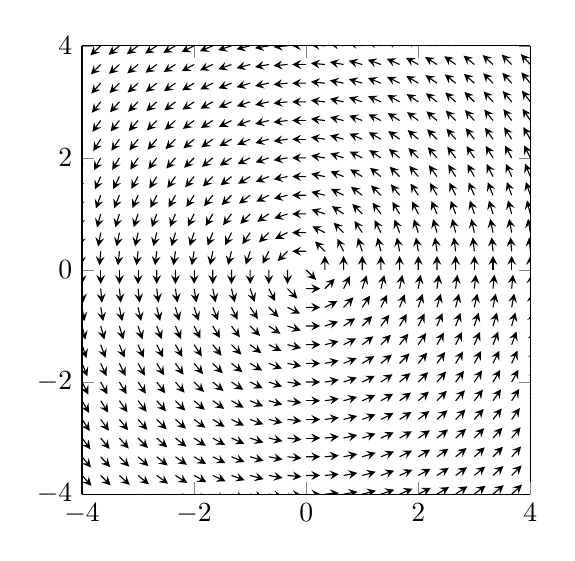
\begin{tikzpicture}
    \begin{axis}[
        xmin = -4, xmax = 4,
        ymin = -4, ymax = 4,
        zmin = 0, zmax = 1,
        axis equal image,
        view = {0}{90},
    ]
        \addplot3[
            quiver = {
                u = {-y/sqrt(x^2+y^2)},
                v = {x/sqrt(x^2+y^2)},
                scale arrows = 0.25,
            },
            -stealth,
            domain = -4:4,
            domain y = -4:4,
        ] {0};
    \end{axis}
    \end{tikzpicture}
\caption{An example vector field}
\end{figure}

With vector fields, two additional types of integrals arise in the AP Physics curriculum. The first is the \textbf{closed surface integral}, which appears in both of Gauss's laws. It is defined as
\begin{equation}
    \oint_A \mathbf{F} \cdot \dd A,
\end{equation}
where $\mathbf{F}$ is a vector field, and $\dd \vec{A}$ represents the normal through a small area. For the most part, these integrals quickly resolve to $|F|A$, where $A$ is the surface area, as the dot product will trivially collapse since $\theta = 90\degr$. Additionally, there is the \textbf{closed loop integral}, which is similar:
\begin{equation}
    \oint_{\ell} \mathbf{F} \cdot \dd\vec{\ell},
\end{equation}
where $\vec{\ell}$ is the normal through a small length. This appears in Ampere's law, and typically resolves to $|F|L$, where $L$ is the length of the loop.

\end{document}